\documentclass{book}
\usepackage{html,graphics,color}
\title{Minsky Simulation Engine}
\bodytext{bgcolor="white"}
\pagecolor[gray]{1}
\author{}

% prevent having to place annoying mboxes
%begin{latexonly}
%\renewcommand{\htmladdimg}[1]{\resizebox{\textwidth}{!}{\includegraphics{images/#1}}}
\renewcommand{\htmladdimg}[1]{\includegraphics{images/#1}}
%end{latexonly}

%begin{latexonly}
\newcommand{\fwhtmladdimg}[1]{
  \noindent\resizebox{\textwidth}{!}{\htmladdimg{#1}}
}
%end{latexonly}
\begin{htmlonly}
\newcommand{\fwhtmladdimg}[1]{\htmladdimg{#1}}
\end{htmlonly}

%begin{latexonly}
\newcommand{\smhtmladdimg}[1]{
  \resizebox{!}{3ex}{\htmladdimg{#1}}
}
%end{latexonly}
\begin{htmlonly}
\newcommand{\smhtmladdimg}[1]{\htmladdimg{#1}}



\end{htmlonly}

\newcommand{\buttonIcon}[1]{
  \resizebox{!}{2ex}{\includegraphics{images/#1}}
  }

\begin{document}


\chapter{Introduction}

\label{Introduction}\emph{Ravel} is a data analysis program which
is an alternative to spreadsheets and existing business intelligence
programs (Tableau, Power BI, etc.). It has two key features that distinguish
it from all other programs in this space: 
\begin{itemize}
\item The Ravel, a visual representation of multidimensional data that is
far easier to use than Pivot Tables; and
\item Equations that are written as flowcharts, rather than the obscure
cell references of spreadsheets.
\end{itemize}
It also includes the system-dynamics engine \emph{Minsky}, which is
documented here: \ref{Introduction-Minsky}.

Unlike spreadsheets, which are fundamentally limited to two dimensions
(rows and columns), \emph{Ravel} supports an effectively unlimited
number of dimensions. \emph{Ravel}'s key feature---also called a
Ravel---is a visual tool for manipulating and analysing multidimensional
data, which can handle as many dimensions as your data contains. By
contrast, to handle more than 2 dimensions in a spreadsheet, the go to
tool is a {\em Pivot table}, which provides some sort of control over
the slice through the multidimensional {\em hypercube}. Needless the
say, pivot tables are not for the faint of heart!

Ravel is primarily focussed on numerical data, although it is possible
to analyse purely symbolic data in \htmlref{``counter mode''}{counter}.

This is a blank Ravel---a Ravel with no data attached to it. The
axes are indicative examples, and will be replaced by the dimensions
of your data, once you attach a data parameter to the Ravel:

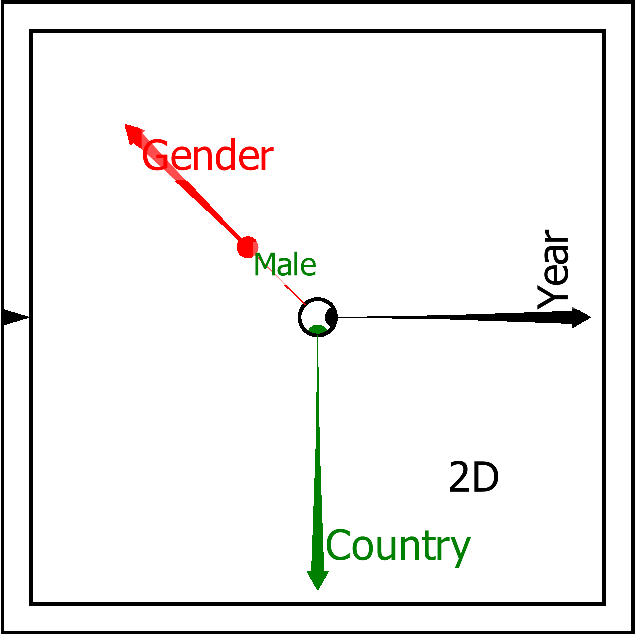
\includegraphics{images/RavelBlank}

To use a Ravel, you first need to import a data file--at present
this must be a CSV file (other data sources will be added in later
releases). Once the data is imported \ref{CSV import}, the data object
can be attached to a Ravel. This is a Ravel with data attached:
\begin{flushleft}
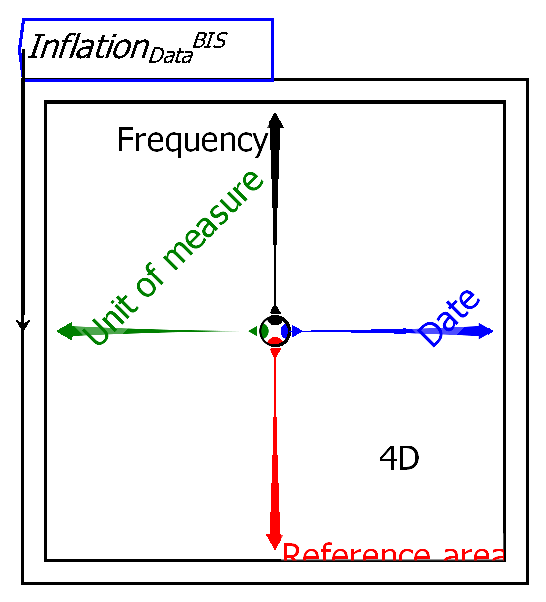
\includegraphics{images/01RavelDataInflation} 
\par\end{flushleft}

There are many ways to manipulate and display data directly from a
Ravel. This is a Ravel with data attached and selected for graphing:
the ``Year on Year Changes'' data is selected from the Unit of Measure
axis; two countries (Japan and the United States) are selected from
the Reference area axis via the \emph{Pick axis slices} command; Monthly
data is chosen from the Frequency axis; and Calipers are applied to
the Date axis to select data from 1960 till 2024.

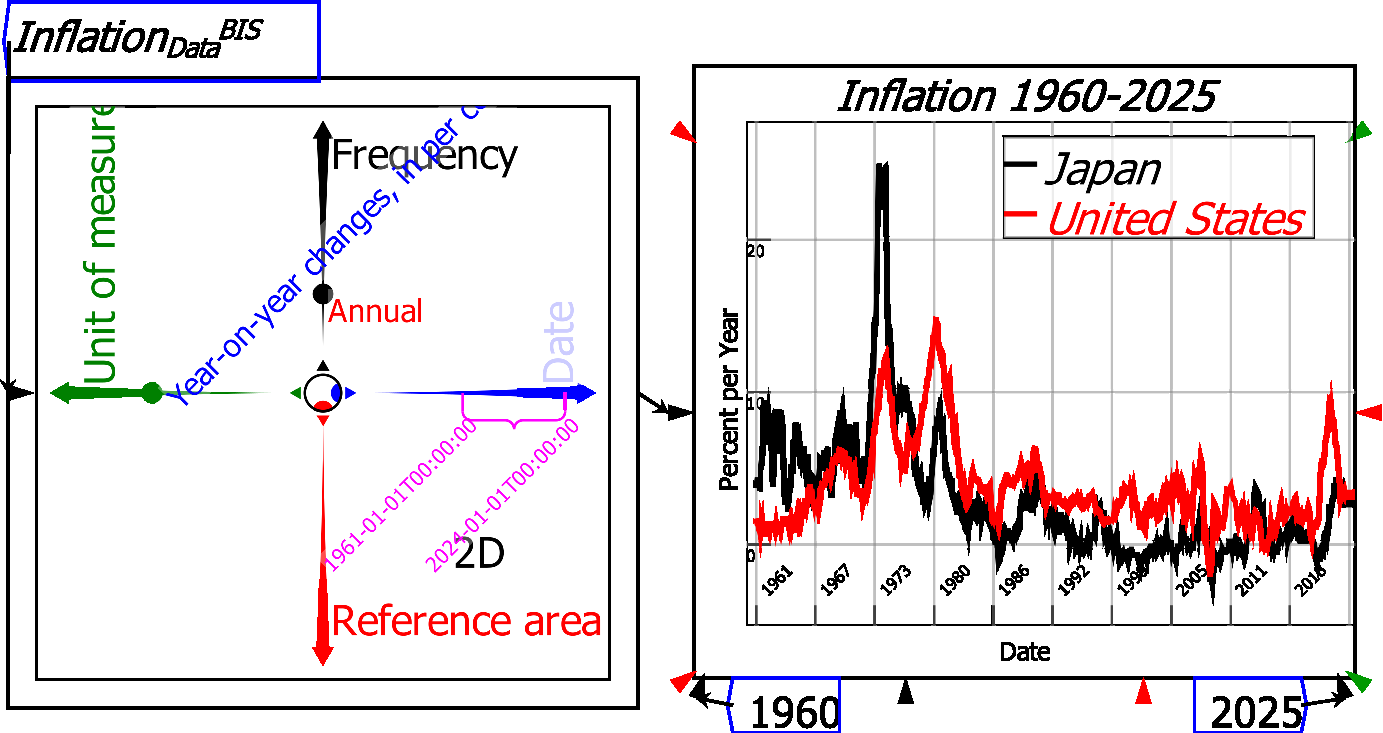
\includegraphics[width=10cm]{images/01BRavelDataInflationSelected}

Ravel the object itself makes it far easier to drill down into and
visualise data than using either a spreadsheet, or the Pivot Tables
that standard Business Intelligence program use.

\emph{Ravel} the program enables easy analysis of data using self-documenting
flowchart formulas.This is a Ravel with data selected--for six countries,
on the annualised monthly inflation rate, for dates from January 2001
till January 2024--and assigned to a variable (``Post2000'').
\noindent \begin{flushleft}
\resizebox{10cm}{!}{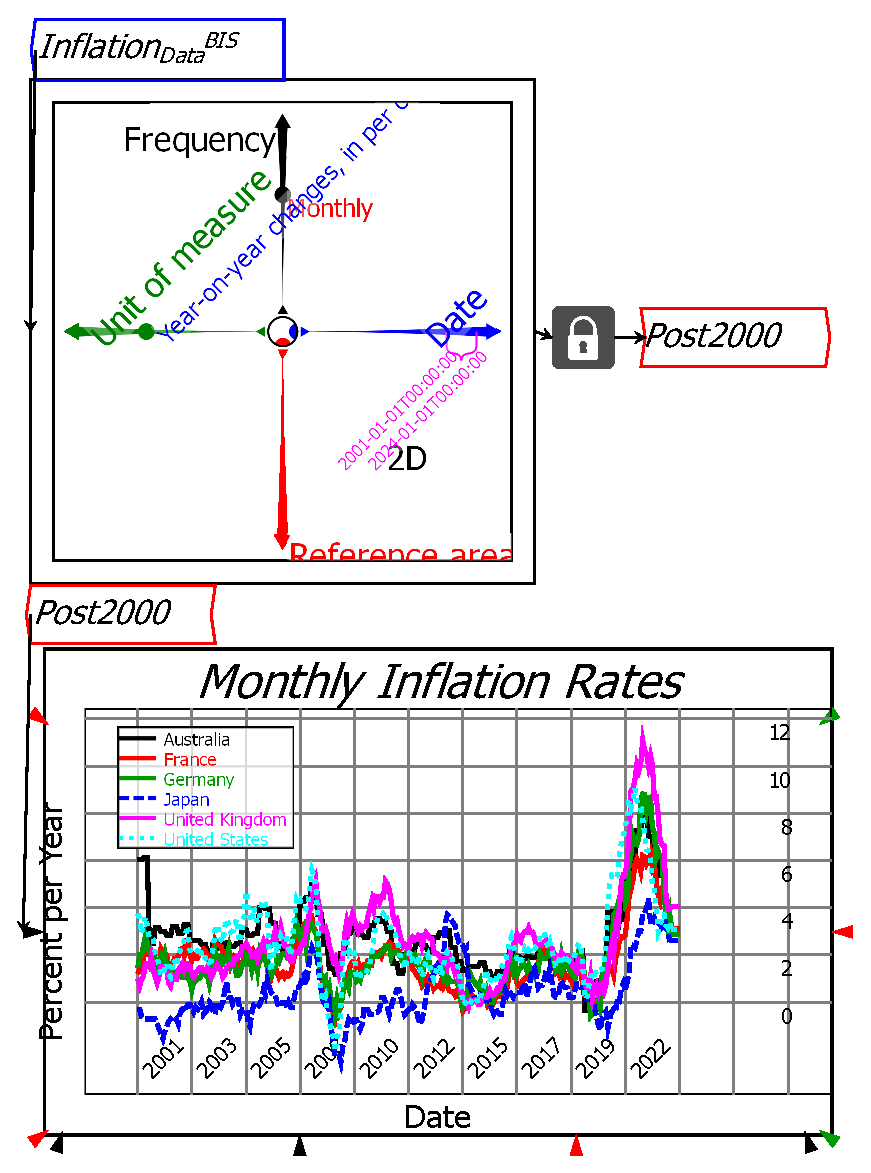
\includegraphics{images/02RavelDataInflationGraphed}} 
\par\end{flushleft}

The data is analyzed by (a) working out the average inflation rate
for the selected countries, and (b) subtracting the average from the
actual inflation rate for each country.

The average inflation rate is calculated using the formula shown below,
where the 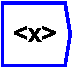
\includegraphics{images/mean}operator works out the average
inflation rate over time for the six countries in the variable \emph{Post2000}
to generate the variable \emph{Inflation}\textsubscript{\emph{Average}}.
This average is then subtracted from the country-specific data in
\emph{Post2000}:

\resizebox{10cm}{!}{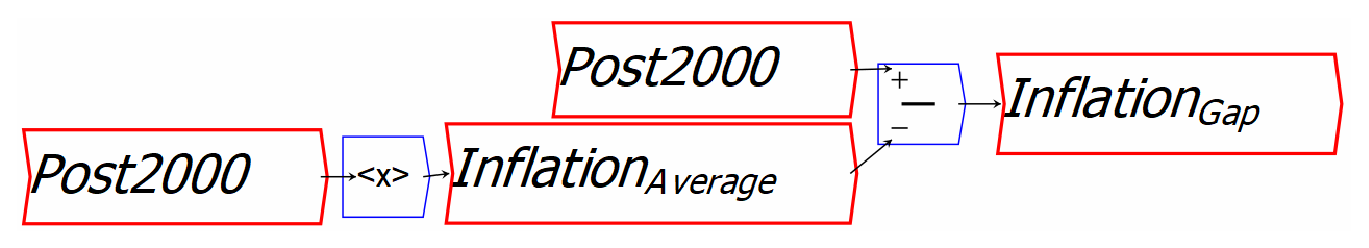
\includegraphics{images/03Formula}} 

This one formula is applied to every country in the Ravel (six countries
in this case) and every quarterly data point (80 quarters). Doing
the same analysis with a spreadsheet would require writing an obscure
cell reference formula and replicating it across 480 cells.

This example shows average inflation outcomes for the six countries,
and the deviation of each of them from the average.
\begin{center}
\resizebox{10cm}{!}{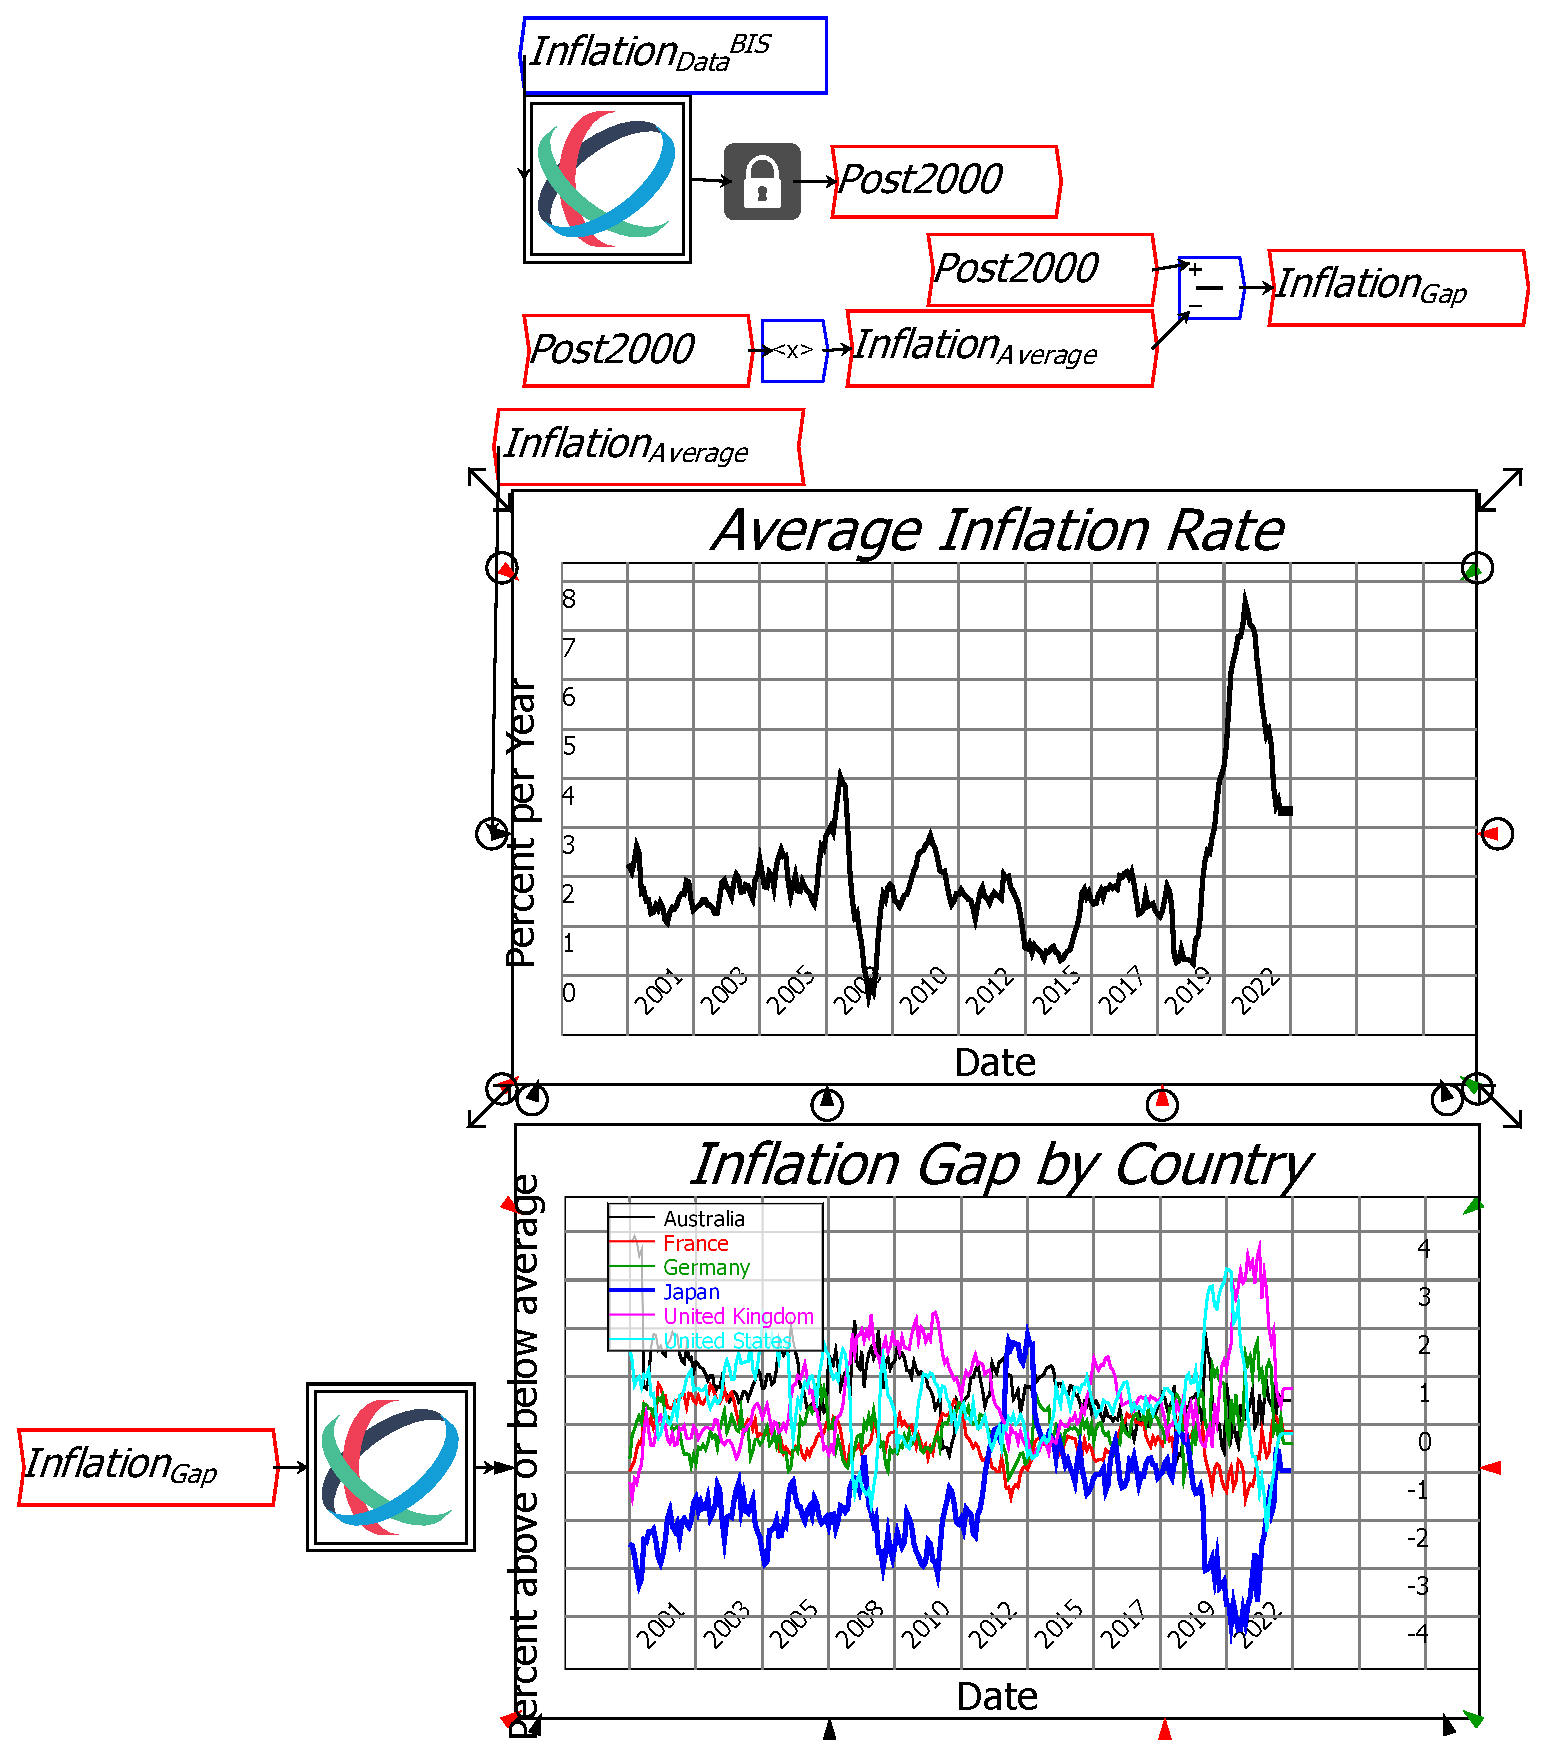
\includegraphics{images/03RavelDataInflationAnalyzed}} 
\par\end{center}

This illustrates the capacity of Ravel to rapidly provide insights
from data--in this case, that the best-performing country during
the post-Covid inflation was Japan, and the worst performing were
the USA and UK. This is noteworthy, because both the USA and UK sharply
increased interest rates with the intention of reducing inflation,
while Japan kept its interest rate constant. Perhaps then, interest
rates aren't effective at controlling inflation rates? 

These examples are drawn from economics, mainly because \emph{Ravel}'s
inventor is an economist (and a contrarian one at that). But \emph{Ravel}
can analyze any data you give it---marketing data, scientific data,
production data, whatever. It can also handle enormous data sets,
far larger than are manageable with Excel.
 
Ravel can handle sparse data---it requires 16 bytes per data point, so
for example, a 16GB computer will technically be able to handle up to a billion
data points, although in practice it is unwise to exceed more than
half that. There is no limit to the number of rows and columns it can
ingest, subject to the overall limit due to available memory, in
contrast to Excel's limits of 1,048,576 rows by 16,384 columns. One
other limit to keep in mind is that the size of the datacube (product
of sizes of all the dimensions) cannot exceed $1.8\times
10^{19}$. This is something to bear in mind when importing data, as
the datacube size increases exponentially with the number of
dimensions.

We hope these examples show how easy it is to turn data into information
using Ravel.

\chapter{Getting Started with Ravel}

Ravel has three main components:
\begin{itemize}
\item The Ravel, a visual representation of your data;
\item Equations expressed as flowcharts; and
\item The system-dynamics engine Minsky
\end{itemize}

\section{System requirements}

Ravel is a proprietary program for data analysis which currently only runs on Windows. It is built on top of Minsky, which is an open source program available for Windows, Mac OS X,and various Linux distributions. Some components of the interface are specific to Minsky. This "Getting Started" guide focuses on the components used by Ravel. For a getting started guide to Minsky, \htmlref{click here}{Getting-Started-Minsky}.

\section{Getting help}

Press the F1 key, or select ``help'' from the context menu. Help is context-sensitive. If you press F1 while the mouse is hovering over a widget--for example, the addition block--then the help window will appear with instructions on how to add elements together.


\section{Components of the Program}

There are 5 main components to the Ravel interface:

\begin{enumerate}
\item  The menus.

  \begin{tabular}{lllllll}
    File & Edit & Bookmarks & Insert & Options & Simulation & Help \\
  \end{tabular}

\item  The Operations controls

\htmladdimg{OperationsControls.png}

\item The Tabs. 

\htmladdimg{Tabs.png}

These are 

\begin{itemize}
\item Wiring, where a model is defined;
\item Equations, which shows you a bitmapped image of all the equations in your model (to see well-formatted equations, use the "File/Export Canvas As" menu, choose LaTeX as the output format, and load the resulting .TeX file into a LaTeX editor);
\item Summary, which provides a detailed and mathematically formatted table of all the components of your model;
\item "Phillips Diagram", which is a Minsky-specific feature not used by Ravel;
\item "Publication", which is a default blank canvas onto which any component of your model can be placed for documentation purposes; and
\item The "+" tab, which enables you to create and name a new Publication tab. Any number of Publication tabs can be created, which lets you save multiple views of a file for different audiences--the one for auditing, say, would be different to the one for marketing, and so on.

\end{itemize}



\item The design icons. These are "widgets" which are placed on the canvas to perform various operations. These include data import parameters, Ravel objects, plots and sheets for displaying data, mathematical operators for analysing your data, and so on. These are explained in detail in the reference sections of the online help.

\fwhtmladdimg{DesignIcons.png}

\item And finally, the Design Canvas--the large drawing area beneath the buttons and icons.

\fwhtmladdimg{RavelCanvas.png}
\end{enumerate}

Some of the elements of the interface are specific to the simulation engine Minsky--for example, the Record and Replay buttons, the Reverse checkbox, "Run-Stop-Step" buttons and the simulation speed slider. These aspects of the interface are explained in the Minsky section of this manual.

\htmladdimg{RunButtons.png}

Others are used by both Ravel and Minsky--for example, the Recalculate button:

\htmladdimg{Recalc.png}

And the Zoom controls, which enable you to Zoom out and In, go to standard Zoom, and fit the document to the visible screen:

\htmladdimg{ZoomControls.png}

\subsection{Menu}
\label{Menu}

The menu controls the basic functions of saving and loading files, default settings for the program, etc. These will alter as the program is developed; the current menu items (as of April 2024) are: 

  \begin{tabular}{lllllll}
    File & Edit & Bookmarks & Insert & Options & Simulation & Help \\
  \end{tabular}

\subsubsection{File}
\label{File}

\begin{description}
\item[About] Tells you the version of Ravel and/or Minsky that you are using.

\item[New System] Clear the design canvas. If you have made changes and haven't saved them, you will be prompted to save before the canvas is cleared.

\item[Open] Open an existing Ravel or Minsky file (Ravel files have the suffix of "rvl". Minsky files have the suffix of ``mky").

\item[Recent Files]\label{recentfiles} Provides a shortcut to some of your previously opened Ravel (or Minsky) files.

\item[Library] Opens a web-based repository of models for the Minsky simulation system. 

\item[Save] Save the current file.

\item[Save As] Save the current file under a new name.

\item[Insert File as Group] Insert a Ravel/Minsky file directly into the current model as a \htmlref{group}{Group}

\item[Dimensional Analysis] This is a Minsky-specific command to check whether definitions in a simulation model are consistent

\item[Export Canvas as] Export the current canvas in svg, pdf, eps, tex, or m format. The current canvas (which varies depending on which Tab you have open) can be exported in a number of different formats:

\begin{itemize}
\item SVG
This is a "vector graphics" format which can be inserted into word processing (such as Word or OpenOffice) or presentation (Powerpoint etc.) documents.
\item PDF
This saves the currently displayed canvas as an Adobe Acrobat file
\item EMF
This saves the canvas in an enhanced form of the WMF (Windows Metafile) vector graphics standard, for use in documentation programs like Powerpoint and Word.
\item Postscript
This saves the canvas in an encapsulated form of PDF 
\item Portable Network Graphics
This saves the canvas in a bitmap file (PNG) for use in paint and photo programs, etc.
\item LaTeX
This exports the equations in a model in a mathematical formatting language called LaTeX. This file can be imported into mathematics programs like MathType to document the mathematical logic in your model. If you are a LaTeX user yourself, you can load this directly into your preferred LaTeX editor.


If your LaTeX implemention doesn't support breqn, untick the \htmlref{wrap long equations option}{wrap-equations}, which can be found in the preferences panel under the options menu.
  \item Matlab
This exports the model as an "m. file" for importing into the algebraic program Matlab. This enables the analysis and simulation of your model in a MatLab compatible system, such as \htmladdnormallinkfoot{MatLab}{https://en.wikipedia.org/wiki/MATLAB} or \htmladdnormallinkfoot{Octave}{http://www.gnu.org/software/octave/}.


\end{itemize}


\item[Log simulation] This Minsky-specific command outputs the results of simulated variables into a CSV data file for later use in other programs.

\item[Recording] This Minsky-specific command records the states of a model as it is being built for later replay.

\item[Replay recording] This Minsky-specific command replays a recording of model states.

\item[Quit] Exit the program. Ravel will check to see whether you have saved your changes. If you have, the program will close; if not, you will get a reminder to save your changes.

\item[Debugging use] Items under the line are intended for developer use, and will not be documented here.

\item[Redraw] Redraw may be useful if the screen gets messed up because of a display bug (all programs have them!). For example, a bug could cause items on the canvas to be scaled differently. Redraw could overcome this problem without requiring you to exit the program.

\end{description}

\subsubsection{Edit}
\label{Edit}

\begin{itemize}
\item\label{edit:undo} Undo and Redo allow you to step back and forward in your editing history. If you undo a few edits, and then change the model at that point, the undo history is then reset to commence with your new edit. Ravel supports the standard Windows shortcuts of control-Z for undo and control-Y for redo.

\item\label{edit:copy} Cut/copy/paste. Selecting, or lassoing a region of the canvas will select a group of icons, which will be shaded to indicate the selected items. Wires joining two selected items will also be selected. Note that, compatible with X-windows, selecting automatically performs a copy, so the copy operation is strictly redundant, but provided for users familiar with systems where an explicit copy request is required. Cut deletes the selected items. Paste will paste the items in the clipboard as a \htmlref{group}{Group} into the current model. Ravel supports the Windows-standard shortcut keys of control-C for copy, control-X for cut (which deletes the entity at the current location and creates a copy for pasting elsewhere) and control-V for paste.

%begin{latexonly}
\begin{tabular}{ccc}
\resizebox{0.45\textwidth}{!}{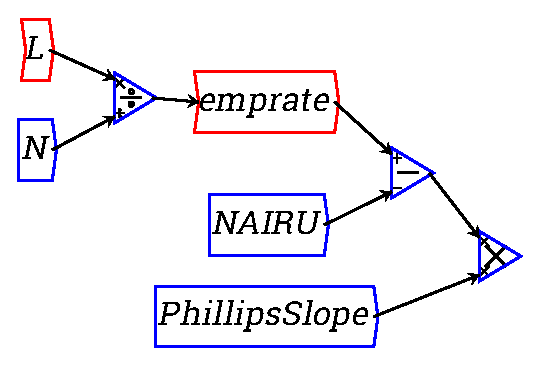
\includegraphics{images/selectionExamplePrior.eps}} & 
\raisebox{1.5cm}{$\Rightarrow$} &
\resizebox{0.45\textwidth}{!}{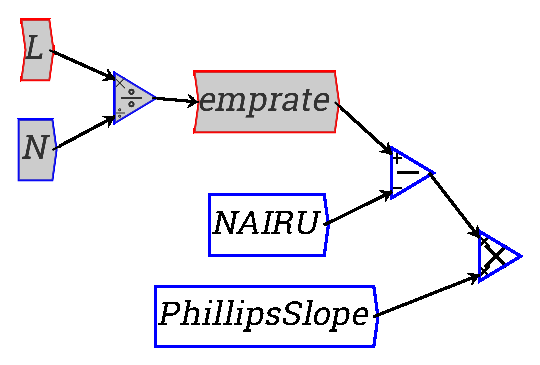
\includegraphics{images/selectionExamplePost.eps}}\\
\end{tabular}
%end{latexonly}
\begin{rawhtml}
<table>
<tr>
<td><img src="selectionExamplePrior.png"></td>
<td><big>&#x21d2;</big></td>
<td><img src="selectionExamplePost.png"></td>
</tr>
</table>
\end{rawhtml}

\item\label{edit:group} Group selection. Create a \htmlref{group}{Group} using the contents of the selection. Groups allow you to organise more complicated systems components into aggregated modules that make the overall system more comprehensible. In Ravel, groups can be used to, for example, collect all the file importing operations into a Group, thus removing these detail of these operations from the top level view. This reduces the complexity of a canvas, which can make it easier for a viewer to focus on the analysis that the program is actually doing.

\end{itemize}

\subsubsection{Bookmarks}
\label{Bookmarks}
Bookmarks store the location and scaling of a model for future reference. This is an alternative to grouping as a means to organize a model. To create a bookmark, move the canvas and zoom it to the level at which all the items you wish to bookmark are visible. Then click on the Bookmark menu and choose "Bookmark this position". Give the Bookmark a name and it will be added to this menu. To move to that location in the model, click on this Bookmark name. Bookmarks can be deleted using the "Delete bookmark" sub-menu.

\subsubsection{Insert}
\label{Insert}

This menu contains all the \htmlref{mathematical operator blocks}{Operations} used in Ravel, and enables you to place those operators on the Canvas. You can get the same effect by clicking on the Design Icons. A Ravel can be inserted from this menu, as can Minsky-specific tools like \htmlref{Godley table items}{godley} and \htmlref{Plots}{PlotWidget}.


\subsubsection{Options}
\label{Options}

The options menu allows you to customise aspects of Ravel and Minsky. At the moment most options pertain to Minsky rather than Ravel, but this will change as Ravel increases in complexity. In this section of the manual we ignore options pertaining only to Minsky; these are covered in \htmlref{Getting-Started-Minsky}{Getting-Started-Minsky}

\begin{description}
\item[Preferences]\mbox{}

\begin{itemize}
\item Number of recent files to display --- this determines how many previously edited files are displayed on the \htmlref{recentfiles}{recentfiles} menu.
\item\label{wrap-equations} Wrap long equations in LaTeX export. If ticked, Ravel \& Minsky will use the LaTeX "breqn" package to produce nicer looking automatically line-wrapped formulae. Because not all LaTeX implementations are guaranteed to support breqn, untick this option if you encounter problems.
\item\label{font} select a font for variable names, parameter names, etc.
\end{itemize}

\item[Background colour] --- select a colour from which a colour scheme is computed.

\end{description}

\subsubsection{Simulation}
These commands are specific to Minsky and control how a model is simulated. They are covered in the Minsky component of this manual.
\subsubsection{Help}
\label{Help}

Provides an in-program link to this manual. Note that pressing F1 will also launch help windows in a context-sensitive way. That is, it will open the relevant help section for whatever object the mouse is currently hovering over. Similarly, each item on the canvas has a help menu item in the context menu relevant for that item.

\subsection{Record/Replay Buttons}
\label{RecReplayButtons}

\htmladdimg{recReplayButtons.png}

These buttons control the recording / replay mode of Minsky. You can record your interactions with Minsky, and replay those interactions for demonstration/presentation purposes. These commands are specific to Minsky and are covered in the Minsky component of this manual.

\subsection{Recalculate button}
\label {Recalculate}

\htmladdimg{recalculate.png}

The recalculate button computes the values of all variables in a model. Ravel will periodically recalculate, but this is a useful option if you wish to immediately see the results of a calculation.

\subsection{Run Buttons}
\label{RunButtons}

\htmladdimg{NewItem15.png}

These commands are specific to Minsky and are covered in the Minsky component of this manual.


\subsection{Speed slider}
\label{Speedslider}

\begin{center}
\htmladdimg{NewItem16.png}
\end{center}

The speed slider controls the rate at which a model is simulated. These commands are specific to Minsky and are covered in the Minsky component of this manual.

\subsection{Zoom buttons}
\label{ZoomButtons}

\begin{center}
\htmladdimg{NewItem17.png}
\end{center}

The Zoom buttons zoom in and out on the wiring canvas. The same functionality is accessed via the mouse scroll wheel. The reset zoom button \buttonIcon{zoomOrig.eps} resets the zoom level to 1, and also recentres the canvas. It can also be used to recentre the equation view.

The Zoom to Fit button zooms the model so that it just fits in the current canvas window.

\subsection{Simulation time}
\label{SimTime}

In the right hand top corner is a textual display of the current simulation time $t$, and the current (adaptive) difference between iterations $\Delta t$. This information is specific to a Minsky simulation model.

\subsection{Wiring and Equations Tabs}
\label{WiringEquationsTab}\label{tabs:wiring}

\htmladdimg{WiringEquationsTab.png}

This allows you to switch between the visual block diagram wiring view and other views of your document.

\begin{itemize}
\item[Wiring]
This is Ravel's design canvas, where you import data, analyse it using Ravel's mathematical operators and functions, and produce visualisations using Plots and Sheets.
\item[Equations]
As you analyse a model using the flowchart operators in Ravel, the program converts the flowchart logic into standard mathematical formulas. This Tab gives you an instant view of the mathematical logic in your model.
\item[Summary]
This tab provides a structured view of all the equations in a model, with details about the number of dimensions and values in a formula.

For example, this model imports data from the Bank of International Assessments, separates the data into a number of variables, and uses data on debt in domestic currency and debt as a percentage of GDP to derive GDP in domestic currency data.

\includegraphics{images/DebtCalcGDPexample.png}

This is the Summary Tab for that model, showing the variable names, their mathematical definitions, their dimensions, and any initial values assigned to them.

\includegraphics{images/DebtCalcGDPexampleSummaryTab.png}

\item[Phillips Diagram]
This is a Minsky-specific feature which is covered in the Minsky section of this manual.
\item[Publication]
Publication Tabs allow you to place specific items from the Wiring diagram onto a documentation canvas. The default Tab is called "Publication", and additional user-named Tabs can be added using the "+" Tab.

To place an item on a Publication Tab, right-click on it on the Wiring Tab, and then click on "Add item to a publication tab". Click on the desired named tab from the resulting menu. The item will then be placed in the top-left-hand corner of the selected Tab. You can then place it wherever you want on the Publication Tab.

\item[+]
This creates a new tab. Provide a name in the form and press Enter or click OK and the new Tab will be created.
\end{itemize}


\subsection{Design Icons}

\fwhtmladdimg{NewItem18.png}

These are the ``nuts and bolts'' of data analysis using Ravel, and model-building using Minsky. There is a substantial number of icons, and this number will grow over time as more data analysis features are added.

The essential icons for Ravel are the first two: Import Data \buttonIcon{importData.eps} and insert a Ravel \buttonIcon{RavelIcon.png}. 

\begin{description}
\item[Import data] \buttonIcon{importData.eps} Opens an import CSV file dialog, which allows a CSV file to be loaded into a parameter in Ravel (the default name of the parameter is the name of the file being imported). See \htmlref{Importing CSV files}{Operation:csvImport} for full details. After a data file is imported, the next step is to attach it to a Ravel.

\item[Ravel] \buttonIcon{RavelIcon.png}. This places a Ravel on the wiring canvas. The first time this is done in a document, the Ravel is displayed full-size in Edit mode. Subsequent Ravels are displayed in icon mode. For full details on using a Ravel see \htmlref{Ravel}{Ravel}.
  
\item[Plot widget] \buttonIcon{plot.eps} Add \htmlref{plots}{PlotWidget} to the canvas.

\item[Sheet widget] \buttonIcon{sheet.eps} Add a \htmlref{sheet}{Sheet} to the canvas.

\item[Variable]  \buttonIcon{var.eps}. \label{Variable}

This is a pop-up menu, which gives access to the form that creates variables, constants and parameters, and access to the Browser, which is a window that lists all the variables and parameters in a model, and enables them to be placed on the wiring canvas.

Variables are entities whose value changes as a function of time and its relationship with other entities in your model. Click on it and a variable definition window will appear:

\begin{center}
\scalebox{0.5}{\htmladdimg{NewItem32.png}}
\end{center}

The only essential step here is providing a name for the Variable.

Ravel supports the LaTeX language for naming variables (and parameters), which enables you to:

\begin{itemize}
\item Use subscripts and superscripts. The character following an underscore character \_\ is subscripted, while the character following a caret symbol \^\ is superscripted. If the \_\ or \^\ is followed by text in parentheses (curly brackets) \{\}, then all the text within the parentheses is superscripted or subscripted; and
\item Use Greek characters. The English name for a Greek letter (alpha, beta, gamma), preceded by a backslash character $\backslash$ generates the equivalent Greek letter as part of a variable's name  ($\alpha, \beta, \gamma$);

\end{itemize}

This enables more readable variables to be defined, such as, for example $\Delta{Sales}_{Product}^{State}$.

You can also enter a value for it (and a rotation in degrees), but these can be omitted. In a dynamic model, the value will be generated by the model itself, provided its input is wired.


When you click on OK (or press Enter), the newly named variable will appear in the top left hand corner of the Canvas. Move the mouse cursor to where you want to place the variable on the Canvas, click, and it will be placed in that location.


Constants are entities whose value is unaffected by the simulation or other entities in the model. Click on it and a constant definition window will appear:

\begin{center}
\scalebox{0.5}{\htmladdimg{NewItem34.png}}
\end{center}

The only essential element here is its value. You can also specify its rotation on the Canvas in degrees. You can vary the value of a constant or parameter using the arrow keys or the slider button on top of a constant or parameter.

A constant is just a type of variable, which also include parameters (named constants), flow variables, stock variables and integration variables. In fact there is no real conceptual difference between creating a constant or creating a variable, as you can switch the type using the type field.

Like the variable and constant button, the parameter button creates a variable defaulting to the parameter type. Parameters differ from flow variables in not having an input port, and differ from constants in having a name and being controllable by a slider during simulation.

\item[Lock] Lock widgets \buttonIcon{LockIcon.png} are used with \htmlref{Ravels}{Ravel}. A lock keeps a record of the current state of a Ravel: the items selected on its axes, the effect of calipers in selecting data ranges, and so on. You can then manipulate the Ravel without changing the output from the Lock, which can be assigned to a variable for further use. You can also impose the state of a Lock on its associated Ravel.

\item[Notes] Add \htmlref{textual annotations}{Notes}

\item[Time] \buttonIcon{time.eps} embeds a reference to the simulation time on the Canvas. This is a Minsky-specific feature.

\item[Binary operations] \buttonIcon{BinaryButton.png}. These execute the stated binary mathematical operations: operations that require two (or more) inputs. Where appropriate, each input port to a binary operator can take multiple wires---so that to add five numbers together, for example, you can wire 1 input to one port on the Add block, and the other four to the other port. The same applies to the subtract, multiply, and divide blocks: multiple inputs to the input ports on the subtract operator are added together, and then the sum of inputs attached to the "-" port is subtracted from the sum of the inputs attached to the "+" port. For the divide block, the product of the inputs to the "*" port is divided by the product of the inputs to the "/" port.

\htmladdimg{BinaryOperators.png}


Min \& Max Functions. These take the minimum and maximum values, respectively. These also allow multiple wires per input. The sum of the inputs to one port is compared to the sum of the inputs on the other.

Pow and log. These are binary operations (taking just two arguments). In the case of the power operation, the exponent is the top port, and the argument to be raised to that exponent is the bottom port. This is indicated by the $x$ and $y$ labels on the ports. In the case of logarithm, the bottom port (labelled $b$) is the base of the logarithm.

Logical Operators $<$ $\le$, =, $\wedge$ $\vee$ $\neg$ (and, or, not)] These return 0 for false and 1 for true.

\item[Unary functions]\buttonIcon{sqrt.eps} These are a fairly standard complement of mathematical functions which take only one input--though this input can have multiple dimensions.

\item[Reduction operations]\buttonIcon{sum.eps} This menu contains operations that reduce a vector to a scalar, or reduce the rank of a tensor. Typically sum, product, any, all etc.

\item[Scans]\buttonIcon{runningSum.eps} These are running sums and the difference operator

\item[Miscellaneous tensor operations]\buttonIcon{outerProduct.eps}
  Any other tensor function not covered elsewhere.

\item[Switch] \buttonIcon{switchIcon.eps} Add \htmlref{a piecewise-defined function block}{SwitchIcon} 
to the canvas. Also known as a hybrid function.

\item[User defined function]\buttonIcon{userFunction.eps} You can
  define \htmlref{your own function}{Operation:userFunction} using an algebraic expression, such as \verb+exp(-x^2+y)+.

\item[Godley Table] \buttonIcon{NewItem29.eps}. \label{GodleyTable} This is the fundamental element of Minsky that is not found (yet) in any other system dynamics program. It is covered in the Minsky chapter of this manual.


\item[Integration] \buttonIcon{int.eps}.\label{Integrate}
  This inserts a variable whose value depends on the integral of other variables in the system. It is discussed further in the Minsky section of the manual.
  
\item[Derivative Operator] \buttonIcon{differentiate.eps} This operator symbolically differentiates its input. It is a component of Minsky which is explained in the Minsky section of this manual.

\end{description}

\subsection{Design Canvas}
\label{DesignCanvas}\label{tabs:Wiring}

The Design Canvas is where you develop your model. A model consists of a number of blocks---imported data in parameters, Ravels, user-defined parameters, variables, constants, mathematical operators and the display elements (plots and sheets)---connected by wires. 

The canvas is {\em zoomable}, either via the zoom buttons on the toolbar, or via the mouse scroll wheel. It is also {\em pannable}, either via the
scroll bars on the right and bottom, or by holding the shift key and left mouse button together. The canvas is effectively unlimited, however the scroll bars treat the canvas as a $10000\time10000$ pixels in size.

\fwhtmladdimg{NewItem19.png}

\subsection{Equations tab}\label{tabs:Equations}

This displays the mathematical representation of the model

\subsection{Summary Tab}\label{tabs:Summary}

This tab provides a summary table of all variables in the system, in a
heirarchical fashion that can be navigated by expanding or hiding
sections by toggling the caret. Each variable shows its name, it
definition, dimensions (for tensor-valued variables), initial
expression, units and current value.

Most of these fields are editable, and usually do the obvious
thing. Changing a variable's name will do a {\em replace all
  instances} operation to update all variables of the same
name. Changing a variable's definition will replace the wiring graph
leading into the variable by a \htmlref{user defined function}{UserFunction} containing your
edited string. At some future point, functionality will be added to
convert a user defined function into a wiring graph.

\subsection{Phillips diagram tab}\label{tabs:Phillips}

This tab implement's Minsky's take on a \htmladdnormallink{Phillips
  diagram showing the stocks and flows in a monetary
  economy}{https://en.wikipedia.org/wiki/Phillips_Machine}. The
Phillips tab shows all the information contained in the Godley tables
of the model - if there aren't any, this tab will be blank.

Initially, all the stocks will be arranged around a circle, with the
flows shown as connecting arrows showing the current direction of the
flow. You can move and rotate the stocks, and bend the flows to make a
pleasing layout. The stocks will be coloured as though filled with a
fluid like Bill Phillip's original analogue computer, and dynamically
updated as the simulation proceeds.

\subsection{Publication tab}\label{tabs:Publication}

Publication tabs allow the creation of dashboards to emphasise certain
aspects of a simulation. For example, you may wish to focus on a
particular plot or Godley table when running the simulation.

Multiple publication tabs can be created by clicking the '+' tab.

Any item from the wiring tab can be added to a publication tab, and
then moved, resized or rotated independently of the item on the wiring
tab. For items that dynamically update, the publication tab will be
updated dynamically during the simulation.

Textual annotation can be added to the publication tab, independently
of any annotations on the wiring tab.

Wires cannot be added to the publication tab, however you can insert
arrows (eg $\rightarrow$) by typing the LaTeX text \verb+\rightarrow+,
and then rotate and scale the arrow to connect parts of the dashboard together.

\subsection{Wires}
\label{Wires}

The wires in a model connect blocks together to define equations. For example, to write an equation for 100/33, you would place a \buttonIcon{const.eps} on the canvas, and give it the value of 100:

\begin{center}
\scalebox{0.5}{\htmladdimg{NewItem122.png}}
\end{center}

Then do the same for 33, and place a divide block on the canvas:

\begin{center}
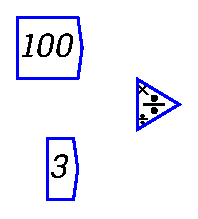
\includegraphics{images/NewItem123.eps}
\end{center}

Then click on the right hand edge of \buttonIcon{const100.eps} and drag to extend the wire to the numerator ($\times$) port of the divide operation.

\begin{center}
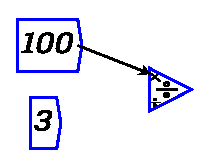
\includegraphics{images/wireExample1.eps}
\end{center}

Finally, add the other wire.
\begin{center}
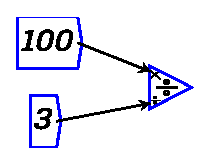
\includegraphics{images/wireExample2.eps}
\end{center}

\section{Working with Ravel}

\subsection{Components in Ravel}

There are several types of components in Ravel
\begin{enumerate}
\item Data storage parameters, which load in data from an external CSV file;
\item Ravels, which take data from a data storage parameter and create a multi-dimensional graphical rendition of the data, with one axis per dimension;
\item Mathematical operators such as plus (+), minus (-), etc. These are all aware of the dimensions of your data, so they act on arrays of data, rather than single cells as with spreadsheet formulas;
\item Constants (or parameters, which are named constants) which are given a value by the user;
\item Variables whose values are calculated by the program during a simulation and depend on the values of constants and other variables; and
\item Groups, which allow components to be grouped into modules that can be used to construct more complex models.
\end{enumerate}


\subsection{Inserting a model component}


There are five ways to insert a component onto the Canvas:
\begin{enumerate}
\item Click on the desired Icon on the Icon Palette, drag the block onto the Canvas and click the mouse where you want to insert it 

\begin{center}
\fwhtmladdimg{NewItem18.png}
\end{center}

\item Choose Insert from the menu and select the desired block there

  \begin{center}
    %begin{latexonly}
    \resizebox{!}{0.6\textheight}{
      %end{latexonly}
      \htmladdimg{NewItem159.png}
     %begin{latexonly}
    }
    %end{latexonly}
  \end{center}
  \newpage
  
\item Right-click on an existing block and choose copy. Then place the copy where you want it on the palette. 

\begin{center}
\htmladdimg{NewItem161.png}
\end{center}

\item Variables can be inserted by typing the variable name on the canvas, and constants can be entered simply by typing the number on the canvas. Similarly, operations can be inserted by typing the operator name (eg \verb+sin+, or \verb+*+). Notes can be inserted by starting the note with a \verb+#+ character.

\item Variables can also be picked from the \htmlref{Variable
    Browser}{VariableBrowser} and placed on the canvas.
\end{enumerate}


\subsection{Creating an equation}

Equations are entered in Ravel graphically. Mathematical operations like addition, multiplication and subtraction are performed by wiring the inputs up to the relevant mathematical block. The output of the block is then the result of the equation. 

For example, a simple equation like
\begin{displaymath}
100/3 = 33.3
\end{displaymath}
is performed in Minsky by defining a constant block with a value of 100, defining another with a value of 3, and wiring them up to a divide-by block. Then attach the output of the divide block to a variable, and run the model by clicking on\smhtmladdimg{NewItem130.png} :

\begin{center}
  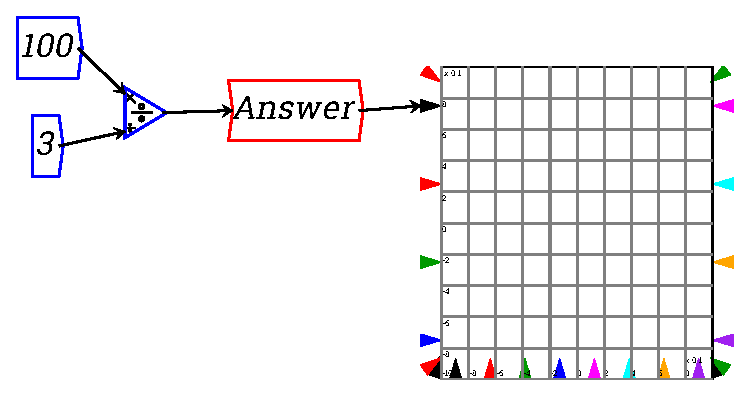
\includegraphics{images/NewItem129.eps}
\end{center}

If you click on the equation tab, you will see that it is:

\begin{displaymath}
\mathrm{Answer}=\frac{100}{3}
\end{displaymath}

\subsection{Wiring components together}

A model is constructed by wiring one component to another in a way that defines an equation. Wires are drawn from the output port of one block to the input port of another. Ports are circles on the blocks to which wires can be attached, which can be seen when hovering the pointer over the block. Variables have an input and an output port; constants and parameters only have an output port. A mathematical operator has as many input ports as are needed to define the operation.

To construct an equation, such as Fred - Wilma = Barney:

Click the mouse near the output port of one block and drag the cursor to the input port of another while holding the mouse button down. An arrow extends out from the output port. Release the mouse button near the required input port of the operator. A connection will be made.

\begin{center}
\includegraphics{images/NewItem181.eps} 
\end{center}

The equation is completed by wiring up the other components in the same way.

\begin{center}
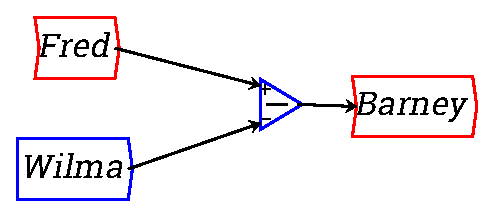
\includegraphics{images/NewItem182.eps} 
\end{center}


\chapter{An Overview of \emph{Ravel}}

\label{tutorial}

\section{Slicing, Dicing and Rotating Data}

A Ravel is a graphical representation of multi-dimensional data. Unlike
a spreadsheet, which has only two dimensions, a Ravel can have as
many dimensions as your data. You manipulate the axes of a Ravel to
select the components of your data that you wish to see, and those
components are then the output of the Ravel, which can be graphed
or displayed directly, or attached to variables which can be further
analysed using the flowchart equation capabilities of \emph{Ravel}.
The Ravel below loads data from the \htmladdnormallink{\emph{Bank of International Settlements}}{https://data.bis.org/bulkdownload}
on house prices. This data has four dimensions:
\begin{description}
\item[Date] Quarterly data from 1927 till 2024: 388 entries 
\item[Unit of Measure] House Price Index where 2010 = 100; 2 entries 
\item[Value] Nominal or Real (CPI-deflated) prices: 2 entries 
\item[Reference Area] Country or Region: 62 entries 
\end{description}
\newpage

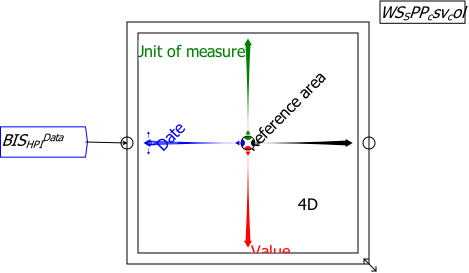
\includegraphics{images/tut00Ravel}

When a Ravel is first attached to data, it outputs the entire data
set---which is indicated by the dimension count \emph{4D} in the
lower right quadrant of this Ravel. You can see this by attaching
a Sheet to the output port of the Ravel:

\noindent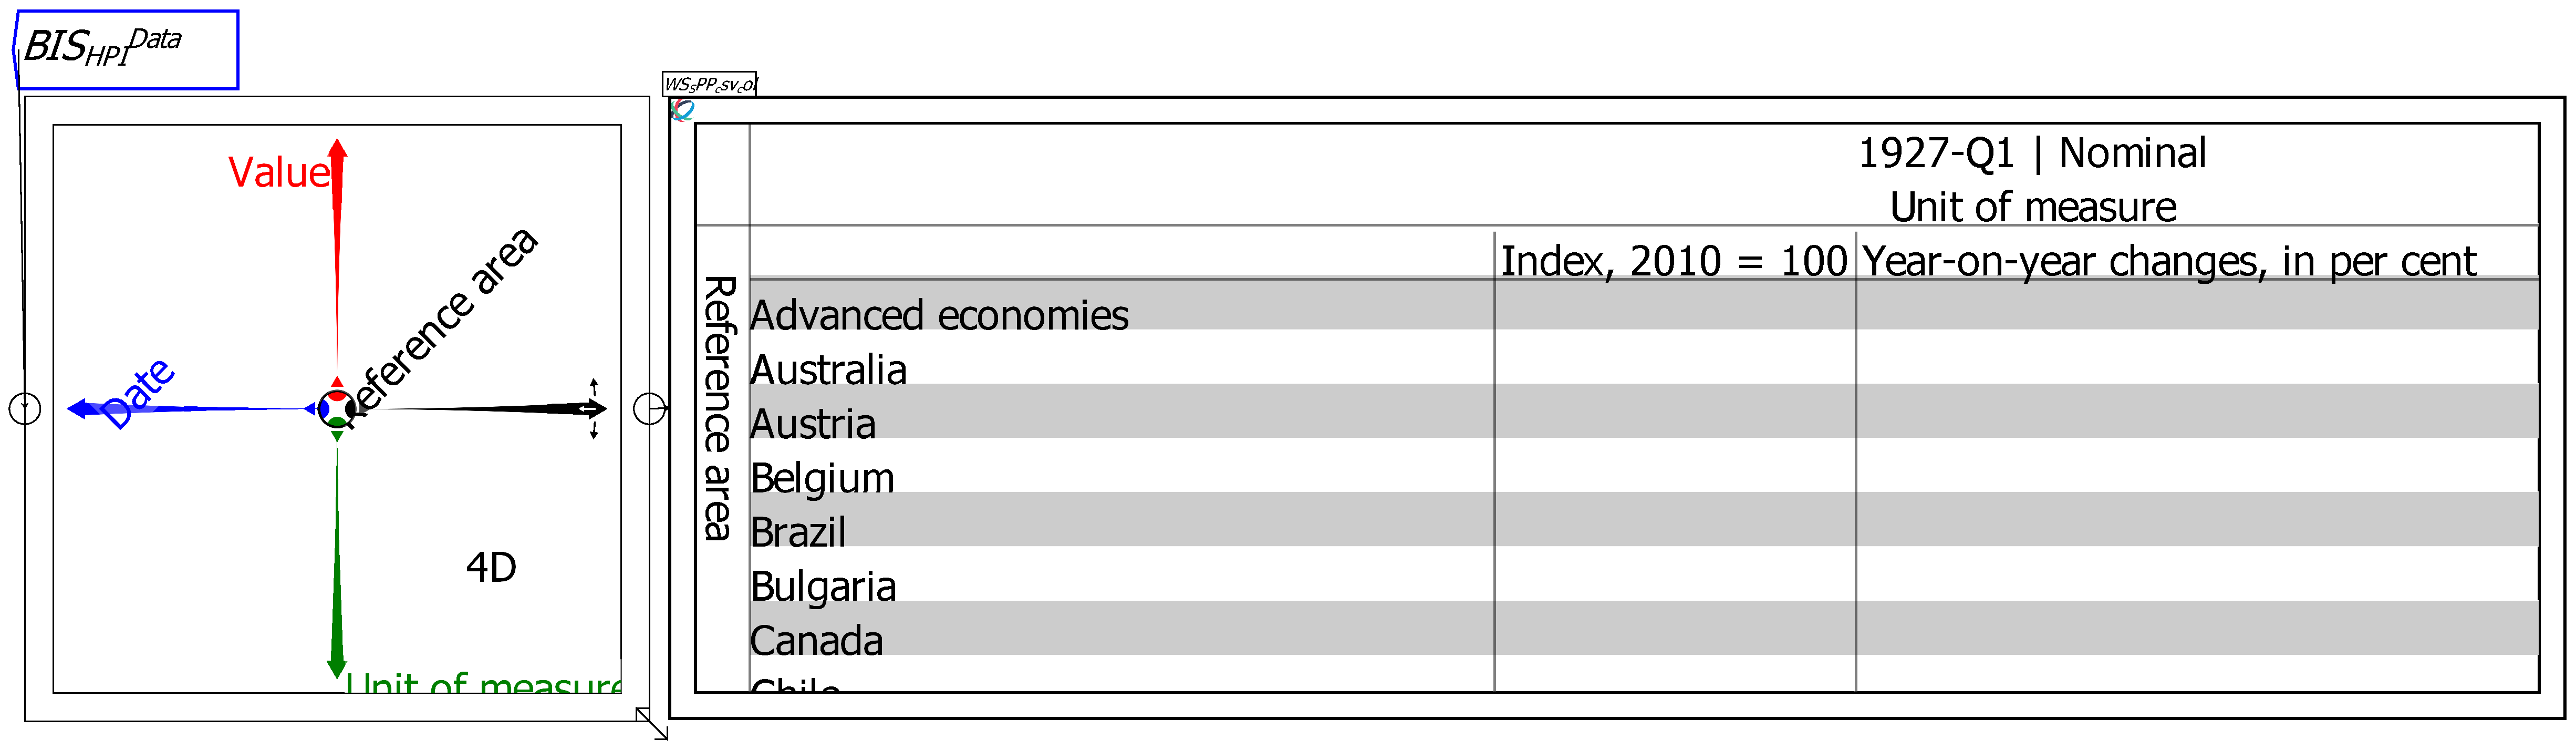
\includegraphics[width=\textwidth]{images/tut01Ravel4DwithSheet}

The right-pointing axis of the Ravel determines what is shown on the
rows of the sheet, while the down-pointing Axes of the Ravel determine
what is shown by the columns. At present these are Reference Area
by Value, and the sheet shows a slice of that data for the first entry
in the Date and Value axes--1927-Q3, and Nominal (unadjusted for
inflation).

It would be more useful to see the data by Reference Area by Date.
To get that view, click the left mouse button on the arrowhead of
the Date axis, hold the button down, and rotate the axis into the
down direction, which is currently occupied by the Value axis. When
you release the mouse button, the Date axis will replace the Unit
of measure axis in the down direction, and the data in the Sheet will
now have countries by rows and Quarters by columns.

\noindent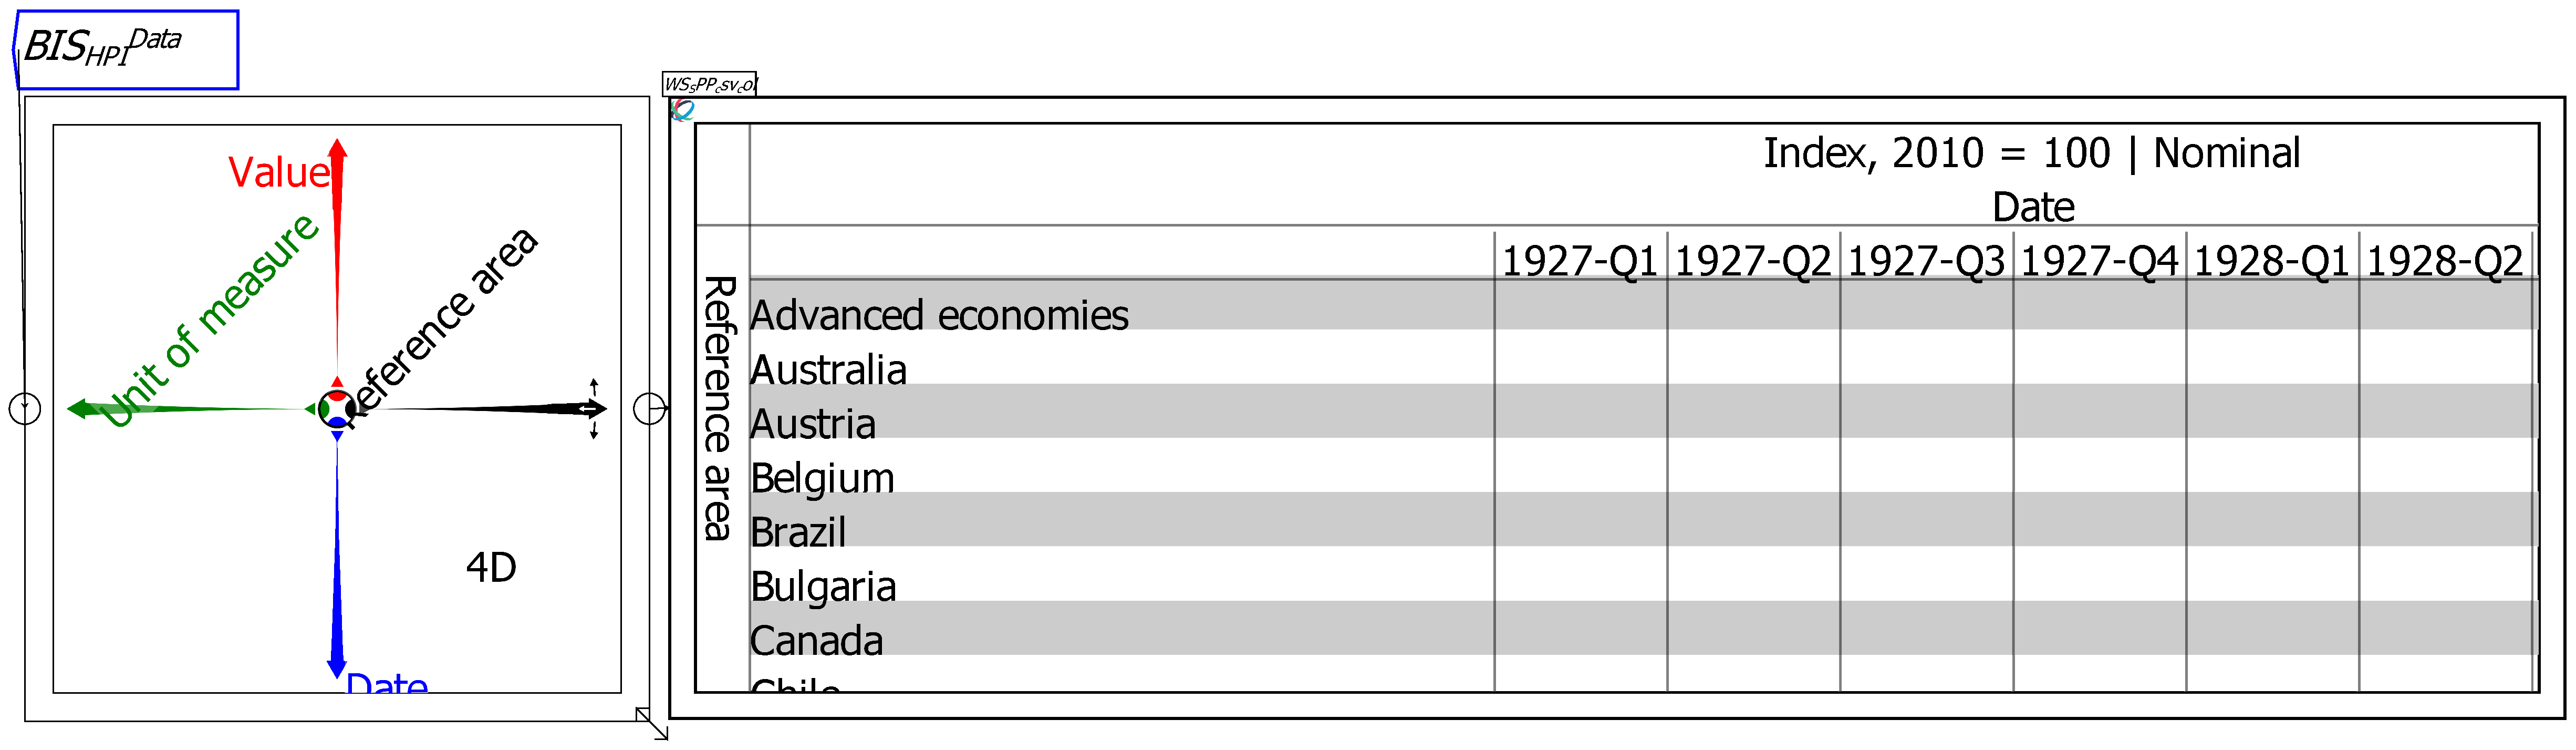
\includegraphics[width=\textwidth]{images/tut02HPI4DwithSheetRotatedCountryDate}

The Sheet is still blank, because there is no data for the current
selections--there is no data for Index for Nominal House Prices in
the very first Quarters of the data (in the years 1927 and 1928) for
the first countries in the file in alphabetical order.

To see data immediately, you can take advantage of a feature of the
Sheet: it can display the first few rows and columns of data (the
default setting), which we call the Head, the last few (the Tail),
or a few of both (Head and Tail). To show the last few rows and columns,
right-click on the Sheet and choose Row Slices/Tail and Column Slices/Tail".
That will then show you the last countries in the data file in alphabetical
order, and the last quarters in the data file.

The data still shows the Nominal Index data, since these are the first
entries in the other two axes. You can control the entry shown using
the selector dots on those two axes: these are the coloured dots that
are currently within the inner circle of the Ravel. Selector dots
can be moved:
\begin{itemize}
\item By using the mouse. Click on a dot and drag it to the required selection;
or 
\item By using the arrow keys. Use the mouse to move the cursor so that
it is hovering over an axis; then use the up or right arrow key to
move the dot out towards the arrowhead on an axis, or the down or
left arrow key to move back towards the center. 
\end{itemize}
To see the Real (CPI-adjusted) annual rate of change of house prices,
use the selector dot on those two axes. That selection is shown below--where
Date has also been rotated to the rows so that Countries are shown
by the columns. This already gives one interesting insight: house
prices were on average falling across advanced countries in 2023.

\noindent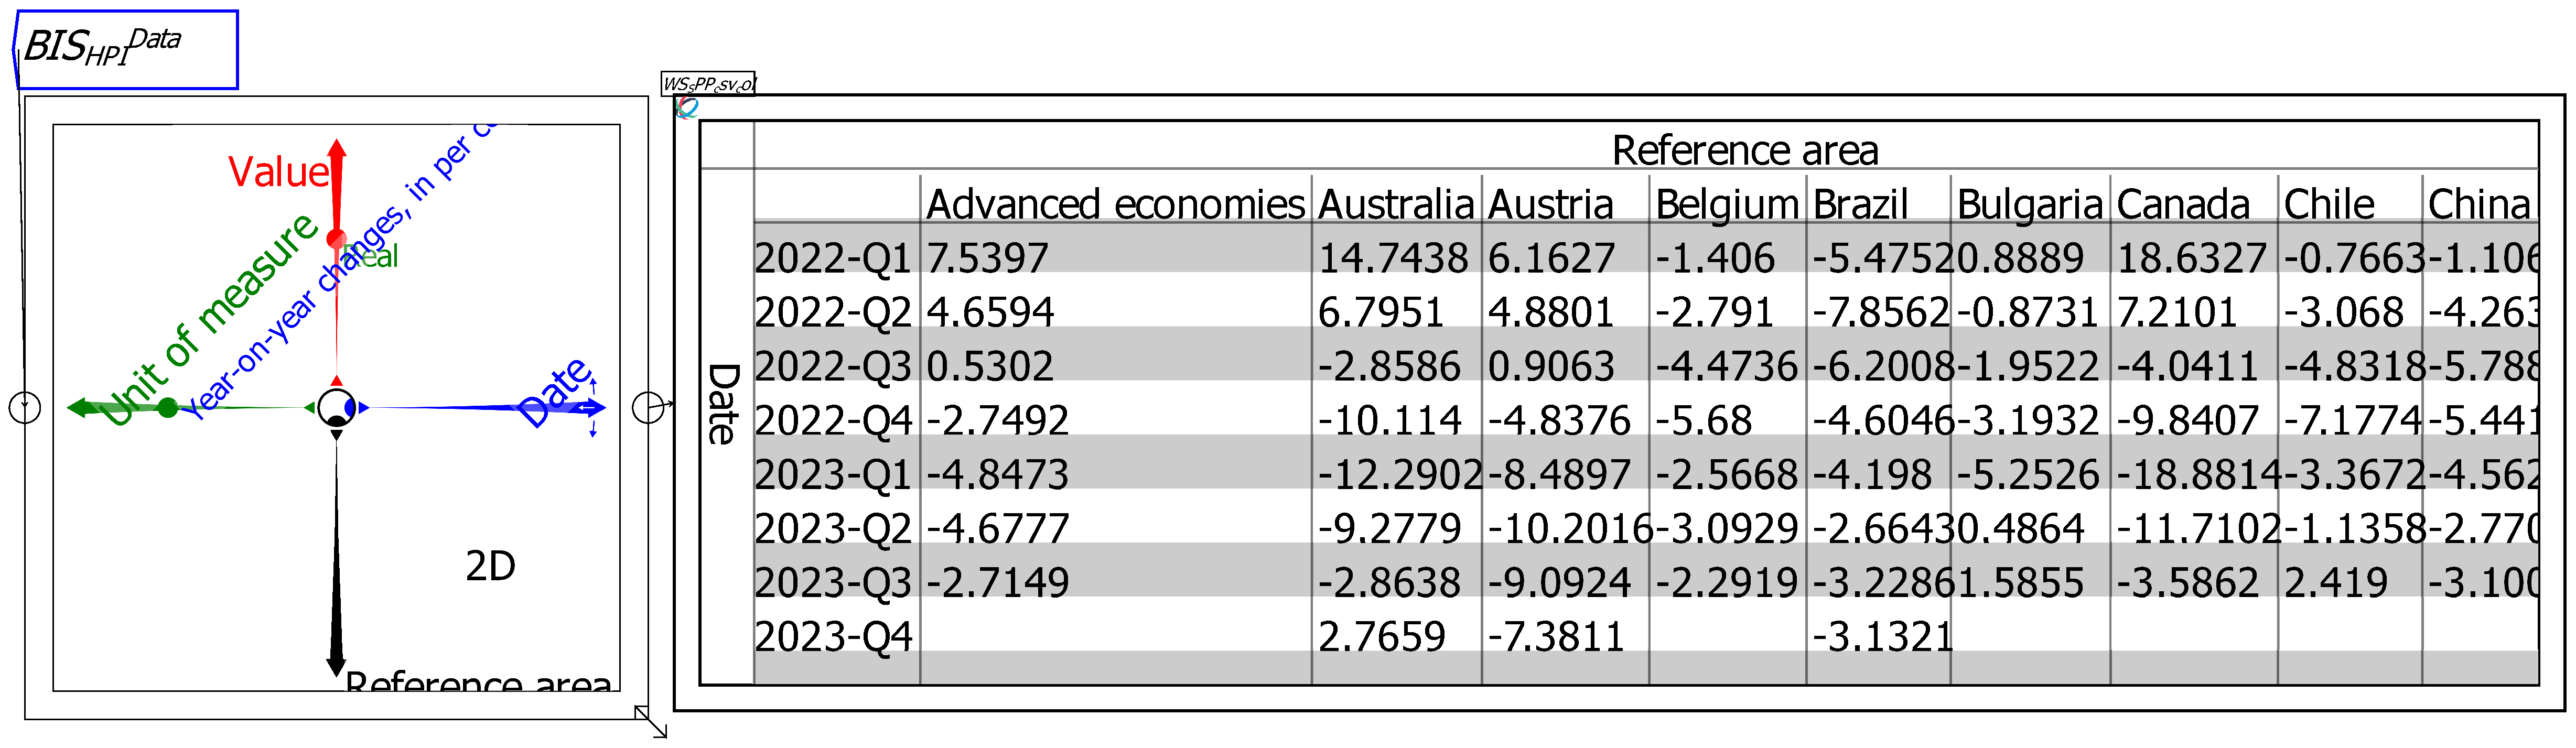
\includegraphics[width=\textwidth]{images/tut04HPI4DwithSheetRotatedCountryDateRealChange}

To really develop insights from your data, you attach the output of
the Ravel to variables, and analyse them using \emph{Ravel}'s flowchart
mathematics formulas.

\section{Attaching Variables to Ravels}

The source data file combines information on House Price Indices (where
the base year is 2010, so all indices are 100 during 2010), and the
annual rate of change of house prices, with data on both Nominal and
Real (CPI-deflated) prices. To analyse the data, it is useful to separate
it into House Price Index information and House Price Inflation information,
and to focus on Real rather than Nominal Prices. That is done by attaching
the output of the Ravel to Locks, and the Locks to named Variables
that you create.

The next image shows two variables $HPI_{Real}$ and $\Delta{HPI}$.
The lock for $\Delta{HPI}$ has been closed, while the lock for $HPI_{Real}$
is still open. Once the lock is closed, the output from that lock
remains the same, even if the selection on the source Ravel is altered.

\noindent\includegraphics[width=\textwidth]{images/tut05HPIandInflationSeparatedLocks}

With the data separated into index and inflation data, we can now
focus on those subsets of the data rather than the entire source file.
The next image shows the source Ravel in icon mode, with the house
price inflation data attached to another Ravel and the currently selected
data displayed in a sheet.

\noindent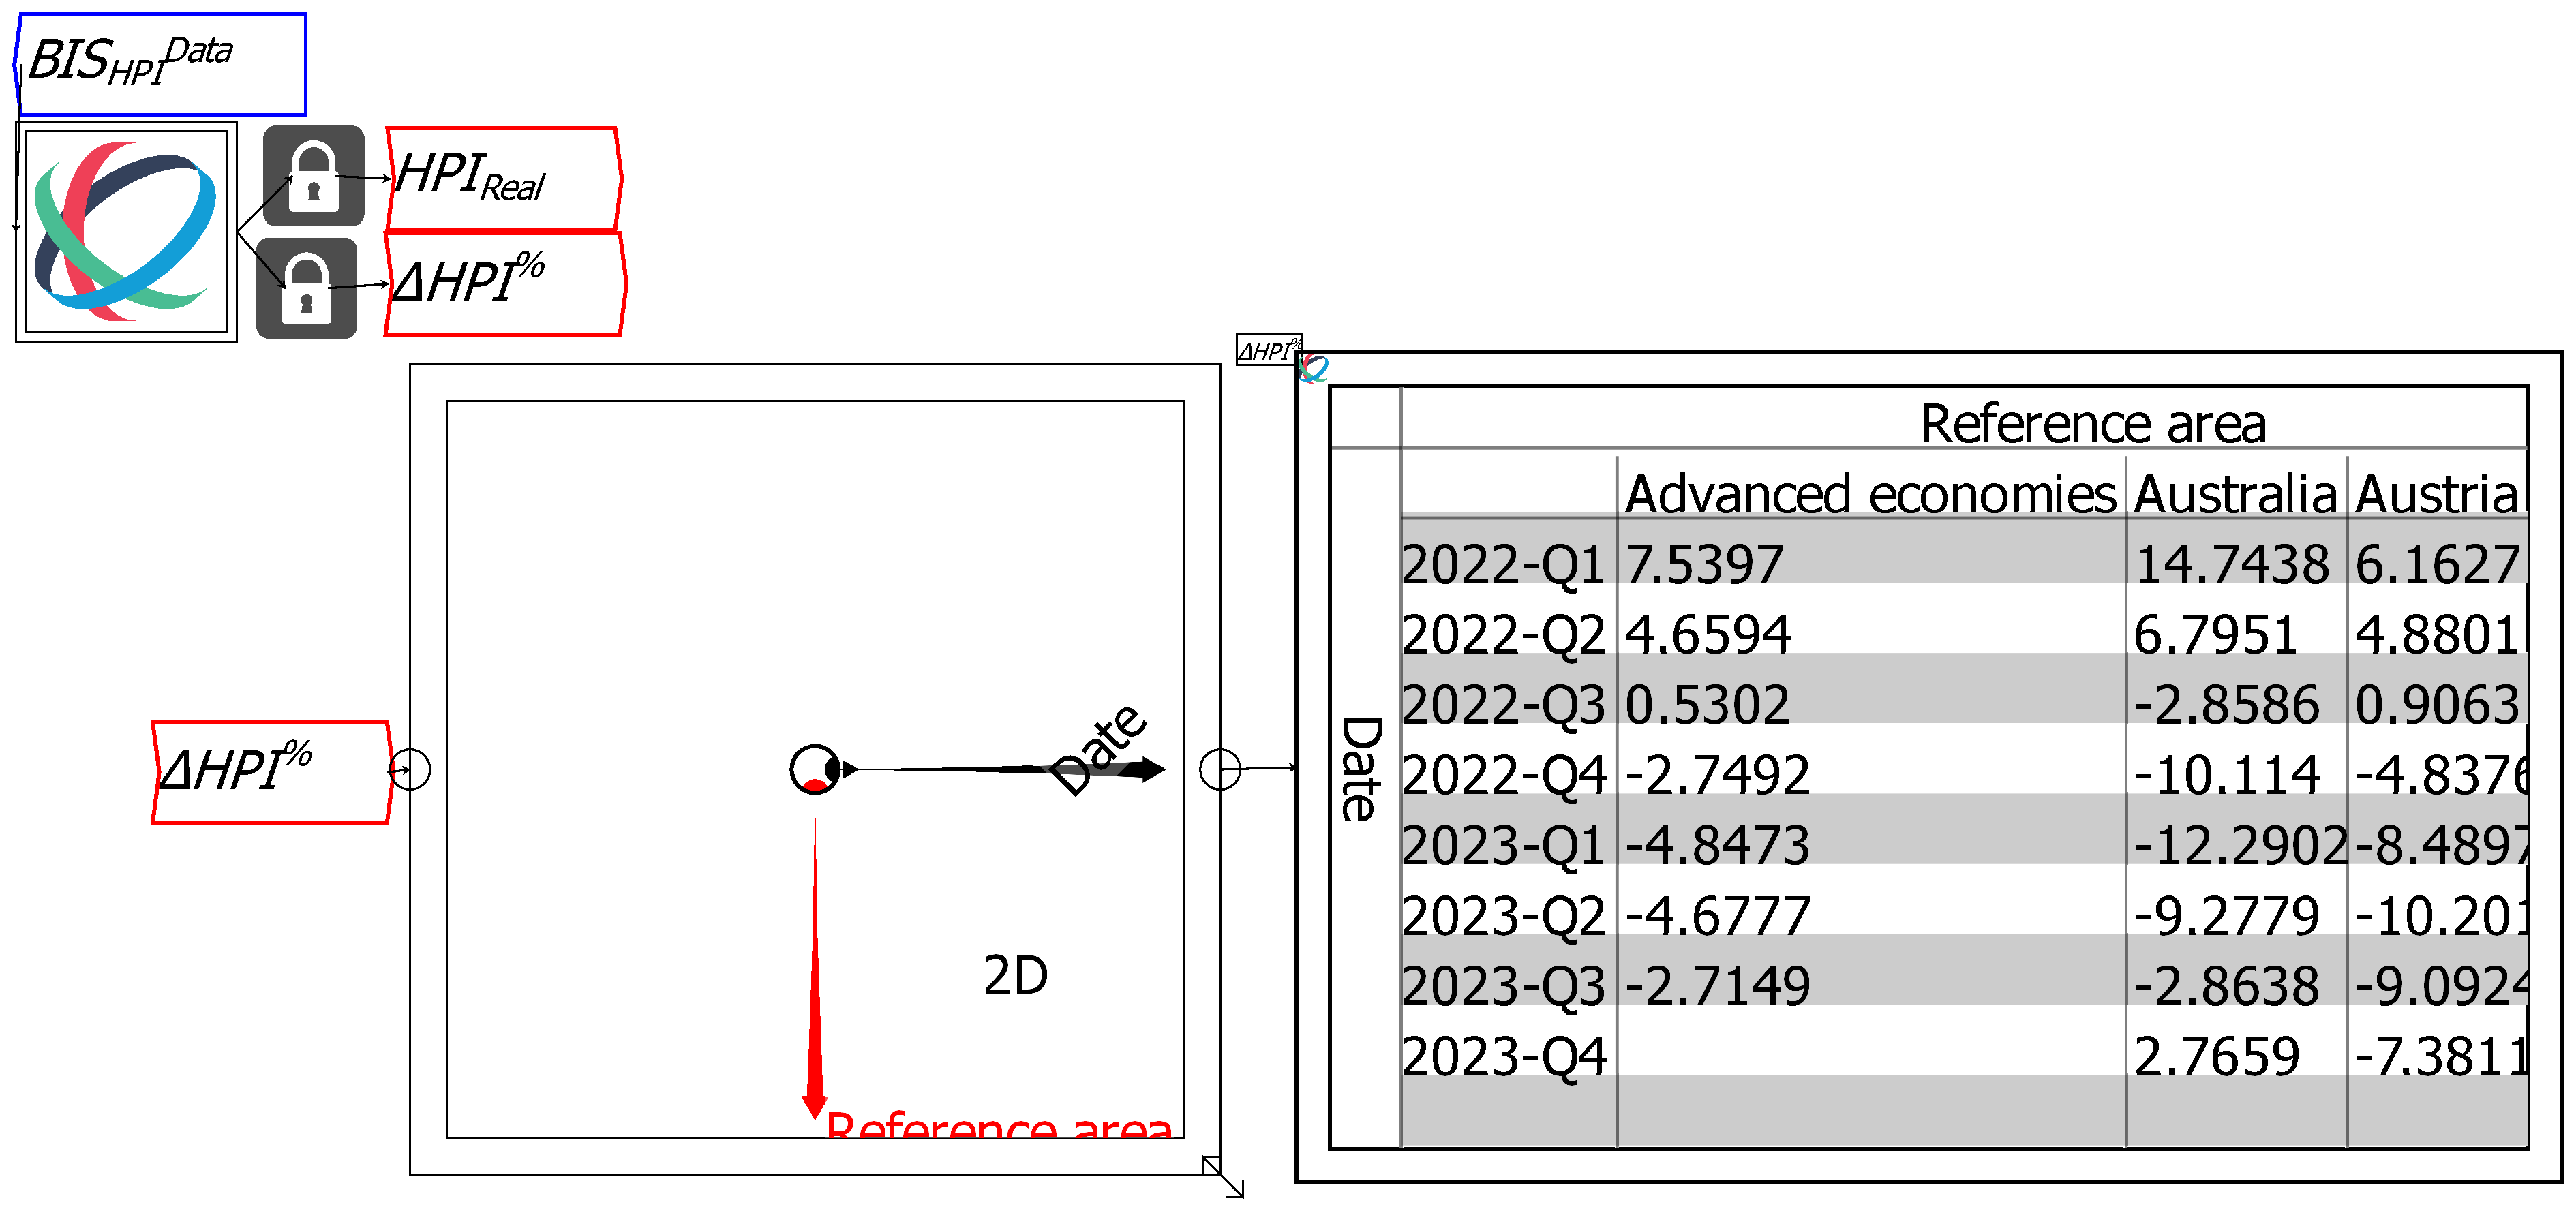
\includegraphics[width=\textwidth]{images/tut06HPIwithVariablesAssigned02DeltaHPI}

The information in the sheet suggests a possibly useful piece of analysis:
why not compare the average for all advanced countries (the first
entry on the Reference Area axis) to each advanced country?

The image below shows the result of attempting to do this by selecting
just the data for ``Advanced Economies'' using the selector dot, and
attaching that to a new variable $\Delta{HPI}_{Advanced}^{Avg}$,
while also selecting a number of advanced economies from the axis
(Australia, Austria, Belgium, etc.) and assigning that to another
variable $\Delta{HPI}_{Advanced}$.

\noindent\includegraphics[width=\textwidth]{images/tut07SeparatingAdvancedAverage}

\section{Basic Analysis using \emph{Ravel}}

Data analysis can be done using the features of a Ravel alone. As
well as enabling the selection of display of different segments of
multidimensional data, you can perform basic data analysis by collapsing
the axes of a Ravel and applying various aggregations:
\begin{enumerate}
\item Summing an axis;
\item Multiplying axis elements by each other;
\item Extracting the maximum or minimum values along an axis; 
\item Calculating the average along an axis;
\item Calculating the standard deviation of an axis; and
\end{enumerate}
More advanced analysis can be performed by attaching the output of
a Ravel to a variable (preferably via a Lock \ref{Lock}, so that
the contents of the variable are unaffected by any subsequent manipulations
of the Ravel), and analysing it using \emph{Ravel}'s mathematical
operators. For more details see \ref{Operations}.

\section{Linking Ravels}

Ravels which have the same dimensions can be linked to each other.
For example, one Ravel may contain inflation data by country by month,
while another contains unemployment data by country by month. If the
two or more Ravels are linked, then selections applied to one Ravel
are applied to the other, which makes it easy to compare these variables
by country over time. For more details see \ref{Linking-Ravels}.

\section{Displaying your results in Sheets and Plots}

Ravels enable the selection and some analysis of data, but don't display
data themselves (however, we will embed Sheets and Plots into Ravels
in future releases of \emph{Ravel}). To see the output of a Ravel,
you need to attach the output of the Ravel (or variables derived from
it) to a Sheet or a Plot. For more details see \ref{Sheet} and \ref{PlotWidget}.

\section{Using Publication Tabs}

Calculations on the Wiring canvas can become too complicated for non-experts
to follow, so Publication tabs exist to enable you to show tailored
views of the results for different audiences---say one Tab for the
Marketing and another for the Accounting divisions of a company. For
details see \ref{tabs:Publication}.

\section{Working with Other Programs \label{Export}}

Though \emph{Ravel} can be used to present results very effectively,
you will sometimes wish to display your results in publication or
presentation software, or to create better-looking plots (Ravel's
Plots will improve dramatically in subsequent releases). You can export
a variety of formats from Ravel:
\begin{enumerate}
\item CSV files, in both columnar and tabular layout;
\item SVG, EPS and EMF vector and PNG bitmapped~graphics files, for use in word
processor and presentation software;
\item PDF format;
\item LaTeX format, for use in mathematical formatting programs like \LaTeX{}
editors and MathType; and
\item .m files, for analysis of the mathematics of a Ravel document in
  Matlab or Octave.
\end{enumerate}
Exporting is done in two main ways:
\begin{enumerate}
\item From the File menu option \emph{Export canvas as}, which exports an
entire canvas (this includes the Equations, Summary and Publication
Tabs)
\item From the context menu for any specific object, such as a Ravel, Variable,
Plot or Sheet.
\end{enumerate}

\section{Importing Data into Ravel}

CSV files typically have some columns that specify the nature
of data, while other columns contain the data itself. \emph{Ravel}
turns the fields specifying the nature of data into \emph{dimensions}
(which become axes of a Ravel), which enables the data to be manipulated
much more effectively than can be done with a spreadsheet. For data
to be imported into \emph{Ravel}, the dimensions must uniquely specify
each data point. This process is controlled by the import tool
\buttonIcon{importData}~, which then brings up the import
form in which you specify which columns to treat as dimensions and
which as data. For more details see \ref{CSV import} and \ref{Operation:csvImport}.

\chapter{Reference}

\section{Operations}\label{Operations}

\subsection{Special
  constants}\label{Operation:euler}\label{Operation:pi}\label{Operation:zero}\label{Operation:one}
\label{Operation:inf}

Some special constants ($e=2.72\ldots$, $\pi=3.14\ldots$, 0, 1,
$\infty$).

\subsection{Percent} \label{Operation:percent} Multiplies input by 100.

\subsection{add +}\label{Operation:add} Add multiple numbers together. The input
  ports allow multiple wires, which are all summed. If an input port
  is unwired, it is equivalent to setting it to zero.

\subsection{subtract $-$}\label{Operation:subtract} Subtract two numbers. The input
  ports allow multiple wires, which are summed prior to the
  subtraction being carried out. If an input port is unwired, it is
  equivalent to setting it to zero. Note the small `+' and `$-$' signs
  on the input ports indicating which terms are added or subtracted from
  the result.

\subsection{multiply $\times$}\label{Operation:multiply} Multiply numbers with each
  other. The input ports allow multiple wires, which are all
  multiplied together. If an input port is unwired, it is equivalent
  to setting it to one.

\subsection{divide $\div$}\label{Operation:divide} Divide a number by another. The
  input ports allow multiple wires, which are multiplied together
  prior to the division being carried out. If an input port is
  unwired, it is equivalent to setting it to one. Note the small
  `$\times$' and `$\div$' signs indicating which port refers to the
  numerator and which the denominator.

\subsection{log}\label{Operation:log} Take the logarithm of the $x$ input port, to
base $b$. The base $b$ needs to be specified --- if the natural
logarithm is desired ($b=e$), use the \htmlref{ln operator}{Operation:ln} instead.

\subsection{pow $x^y$}\label{Operation:pow} Raise one number to the power of another. The
ports are labelled $x$ and $y$, referring the the formula $x^y$.

\subsection{lt $<$}\label{Operation:lt} Returns 0 or 1, depending
  on whether $x<y$ is true (1) or false (0).

\subsection{le $\le$}\label{Operation:le} Returns 0 or 1, depending
  on whether $x\le y$ is true (1) or false (0).

\subsection{eq $=$}\label{Operation:eq} Returns 0 or 1, depending
  on whether $x=y$ is true (1) or false (0).

\subsection{min}\label{Operation:min} Returns the minimum of $x$ and $y$.

\subsection{max}\label{Operation:max} Returns the maximum of $x$ and $y$.

\subsection{and $\wedge$}\label{Operation:and_} Logical and of $x$ and $y$, where
  $x\le 0.5$
  means false, and $x>0.5$ means true. The output is 1 or 0, depending
  on the result being true (1) or false (0) respectively.

\subsection{or $\vee$}\label{Operation:or_} Logical or of $x$ and $y$, where $x\le0.5$
  means false, and $x>0.5$ means true. The output is 1 or 0, depending
  on the result being true (1) or false (0) respectively.

\subsection{not $\neg$}\label{Operation:not_} The output is 1 or 0, depending
  on whether $x\le0.5$ is true (1) or false (0) respectively.

\subsection{time $t$}\label{Operation:time}  Returns the current value
of system time.

\subsection{Gamma $\Gamma$}\label{Operation:Gamma} Returns the Gamma
function of its argument:
\begin{displaymath}
  \Gamma(x)=\int_0^\infty t^{x-1}e^{-t}dt
\end{displaymath}

\subsection{Factorial !}\label{Operation:fact} Returns the factorial
of its argument:
\begin{eqnarray*}
    0!&=&1\\
  n! &=& \prod_{i=1}^n i\\
\end{eqnarray*}
Note:
\begin{displaymath}
  n!=\Gamma(n+1)
\end{displaymath}
which is how it is implemented in Minsky.

\subsection{Polygamma $\psi^{(n)}(x)$}\label{Operation:polygamma} Returns the polygamma function
of the first argument $x$, with the order $n$ being given by the floor
of the second argument.
\begin{displaymath}
  \psi^{(n)}(x)=\frac{d^{n+1}}{dx^{n+1}}\ln\Gamma(x)
\end{displaymath}

It relationship to the derivative of the Gamma function (and
factorials) is why Minsky provides this function.

\subsection{time $t$}\label{Operation:time}  Returns the current value of system time.

\subsection{differentiate $d/dt$}\label{Operation:differentiate}
Symbolically differentiates its input with respect to system time, producing d/dt[input]. 
For further explanation regarding differentiation, see \href{https://en.wikipedia.org/wiki/Derivative}{this wikipedia page}.

%\subsection{data }\label{Operation:data} \buttonIcon{data.eps} A data interpolation
%widget. The data can be imported from a file containing
%two values on each line, eg:
%\begin{quote}
%\begin{tabular}{rr}
%0.1 &0.3\\
%0.5 &0.7\\
%0.9 &1\\
%\end{tabular}
%\end{quote}
%
%If the input is less than the minimum key value (0.1 here), then the
%operation outputs the corresponding value (0.3). Similarly if the
%input is greater than the maximum (0.9), the corresponding value (1)
%is output. If it lies in between two keys (eg 0.2), the the output is
%linearly interpolated (0.4).
%
%Alternatively, the data block can be initialised by a random number
%generator, which is a way of introducing random numbers\index{random
%  numbers} into the simulation. The parameters, the
%minimum and maximum values of the function's domain, and the number of
%random samples over that domain, are all required.
%
%\begin{center}
%  \begin{tabular}{cc}
%  \resizebox{5.17cm}{!}{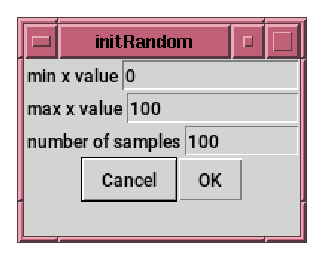
\includegraphics{images/initRandom.eps}} &
%  \resizebox{0.5\textwidth}{!}{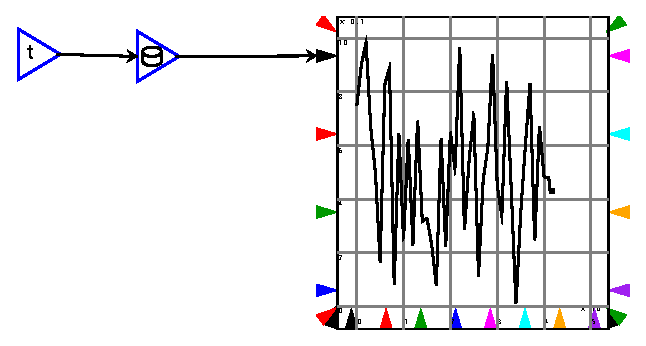
\includegraphics{images/randomExample.eps}}
%  \end{tabular}
%\end{center}
%
%More formally, a data block is an empirical function, based on a table
%of pairs of values ($x_i, y_i, i=1\ldots n, x_{i+1}>x_i$) read in from
%a file. The function's output is linearly interpolated from the data,
%ie:
%\begin{displaymath}
%f(x) = \left\{
%\begin{array}{cl}
%y_1 & x < x_1\\
%y_n & x\geq x_n\\
%\frac{y_i(x_{i+1}-x)+y_{i+1}(x-x_i)}{x_{i+1}-x_i} & x_i \leq x <
%x_{i+1}\\
%\end{array}
%\right.
%\end{displaymath}

\subsection{User defined function}\label{Operation:userFunction}\label{UserFunction}

A user defined function is a functioned defined by an algebraic
expression. Support for this feature is courtesy of the wonderful
\htmladdnormallink{exprtk}{http://www.partow.net/programming/exprtk/index.html}
library developed by Arash Partow.

A user defined function has a {\em name}, {\em parameters} and an {\em
  expression}. Example expressions are things like \verb'x+y' or
\verb'sin(x)'. More details of the sorts of expressions possible can be
found in the \htmlref{User Defined Functions}{ExprTk} section of the
manual.

The parameters are specified as part of the name, so a user defined
function adding x and y would be called \verb'useradd(a,y)' and the
sin example might be called \verb'mysin(x)'. Functions with up to two
arguments can be wired on the canvas. User defined functions can call other
user defined functions, so specifiying more than 2 parameters can be a
useful thing to do. 

\subsection{copy}\label{Operation:copy} This just copies its input to its output,
which is redundant on wiring diagrams, but is needed for internal
purposes.

\subsection{integrate $\int dt$}\label{IntOp}  Creates an integration (or stock)
variable. Editable attributes include the variable's name and its
initial value at $t=0$. The function to be integrated needs to be
connected to the top port. The bottom port can optionally be connected
to a constant, parameter or variable, which is used to specify the
initial value of the integral.

\subsection{sqrt $\surd$}\label{Operation:sqrt} This produces the square root of 
the input value. For example, connecting the value of 9 with the ``sqrt'' block will
produce the value of 3.

\subsection{exp}\label{Operation:exp} Connecting a variable (for example, ``time'')
to this block will produce the exponential function $e^{x}$ where x is the input variable. 

\subsection{ln}\label{Operation:ln} Produces a natural logarithm of the input, to the base of e.
This takes the equation $\log_{e} x$ where ``x'' is the input.

\subsection{sin}\label{Operation:sin} Produces a sine function of the input. For example, 
connecting a ``time'' block to this function, and then to a graph, will produce a sine wave.
For further explanation regarding trigonemtric functions, 
see \href{https://en.wikipedia.org/wiki/Trigonometric_functions}{this wikipedia page}.

\subsection{cos}\label{Operation:cos} Produces a cosine function of the input. For example, 
connecting a ``time'' block to this function, and then to a graph, will produce a cosine wave.
For further explanation regarding trigonemtric functions, 
see \href{https://en.wikipedia.org/wiki/Trigonometric_functions}{this wikipedia page}.

\subsection{tan}\label{Operation:tan} Produces a tangent function of the input. For example, 
connecting a ``time'' block to this function, and then to a graph, will produce a tangent graph.
For further explanation regarding trigonemtric functions, 
see \href{https://en.wikipedia.org/wiki/Trigonometric_functions}{this wikipedia page}.

\subsection{asin}\label{Operation:asin} Produces an arc sine function of the input, 
or the inverse of the sine function. For further explanation regarding trigonemtric functions, 
see \href{https://en.wikipedia.org/wiki/Trigonometric_functions}{this wikipedia page}.

\subsection{acos}\label{Operation:acos} Produces an arc cosine function of the input, 
or the inverse of the cosine function. For further explanation regarding trigonemtric functions, 
see \href{https://en.wikipedia.org/wiki/Trigonometric_functions}{this wikipedia page}.

\subsection{atan}\label{Operation:atan} Produces an arc tangent function of the input, 
or the inverse of the tangent function. For further explanation regarding trigonemtric functions, 
see \href{https://en.wikipedia.org/wiki/Trigonometric_functions}{this wikipedia page}.

\subsection{sinh}\label{Operation:sinh} hyperbolic sine function $\frac{e^x-e^{-x}}2$
\subsection{cosh}\label{Operation:cosh} hyperbolic cosine function $\frac{e^x+e^{-x}}2$
\subsection{tanh}\label{Operation:tanh} hyperbolic tangent function $\frac{e^x-e^{-x}}{e^x+e^{-x}}$
\subsection{abs $|x|$}\label{Operation:abs} absolute value function
\subsection{floor $\lfloor x\rfloor$}\label{Operation:floor} The greatest integer
  less than or equal to $x$.
\subsection{frac}\label{Operation:frac} Fractional part of $x$, ie $x-\lfloor x\rfloor$. 

\section{Tensor operations}\label{tensor operations}\index{tensor|operations}

In the following operations, an axis argument can be supplied in the
operation edit dialog. The axis name is symbolic and available in a
drop down box. If the axis name is not specified, then the operation
will be applied as though the input was flattened (unrolled to a
vector), and then the result reshaped to the original tensor.

\subsection{sum $\sum$}\label{Operation:sum} Sum along a given
axis. 

\subsection{product $\prod$}\label{Operation:product} Multiply along a given axis. 

\subsection{infimum}\label{Operation:infimum} Return the least value
along a given axis. 

\subsection{supremum}\label{Operation:supremum} Return the greatest value
along a given axis. 

\subsection{any}\label{Operation:any} Return 1 if any value
along a given axis is nonzero, otherwise return 0 if all are zero. 

\subsection{all}\label{Operation:all} Return 1 if all values
along a given axis are nonzero, otherwise return 0 if any are zero. 

\subsection{infindex}\label{Operation:infIndex} Return the index of
the least value along a given axis.

\subsection{supindex}\label{Operation:supIndex} Return the index of
the greatest value along a given axis.

\subsection{running sum $\sum+$}\label{Operation:runningSum} Computes
the running sum of the input tensor along a given axis. For example, take
this rank 2 tensor:

\begin{displaymath}
  \left(
  \begin{array}{cccc}
    1& 2& 3& 4 \\
    5& 4& 3& 2 \\
    8& 7& 6& 5
  \end{array}
  \right)
\end{displaymath}

The running sum of this tensor, along the horizontal dimension, is: 

\begin{displaymath}
  \left(
  \begin{array}{cccc}
    1& 3& 6& 10 \\
    5& 9& 12& 14 \\
    8& 15& 21& 26
  \end{array}
  \right)
\end{displaymath}

\subsection{running product $\prod+$}
\label{Operation:runningProduct} Computes the running
product of the input tensor along a given axis. For example, take
this rank 2 tensor:

\begin{displaymath}
  \left(
  \begin{array}{cccc}
    1& 2& 3& 4\\ 
    5& 4& 3& 2\\ 
    8& 7& 6& 5 
  \end{array}
  \right)
\end{displaymath}

The running product of this tensor, along the horizontal dimension, is: 

\begin{displaymath}
  \left(
  \begin{array}{cccc}
    1& 2& 6& 24\\ 
    5& 20& 60& 120\\ 
    8& 56& 336& 1680 
  \end{array}
  \right)
\end{displaymath}

\subsection{difference $\Delta$}\label{Operation:difference}
Computes the nearest neighbour difference along a given direction. The
optional argument can be used to specify the number of neighbours to
skip in computing the differences.

\subsection{index}\label{Operation:index}

Returns the index within the hypecube where the input is true (ie
$>0.5$). For example, where
\begin{eqnarray*}
  \iota(3,3) &=& \left(\begin{array}{ccc}
  0 & 3 & 6 \\
  1 & 4 & 7 \\
  2 & 5 & 8 \\
  \end{array}\right),\\
  \mathrm{idx}(\iota(3,3)<5) &=&
  \left(\begin{array}{ccc}
    0 & 3 &\\
    1 & 4 &\\
    2 & &
  \end{array}\right),\\
\end{eqnarray*}
Note that the output array has the same shape as the input, with
unused values padded with NANs (missing value).

Dimension and argument parameters are unused.


\subsection{gather}\label{Operation:gather}

Gather collects the values at index locations indexed by the second
argument. The output tensor has shape $[i_0, \ldots i_{ir}, a_0,\ldots
a_{j-1},a_{j+1},\ldots a_{ar}]$ where $[a_0,\ldots,a_{ar}]$ is the
shape of the first argument, and $[i_0,\ldots,i_{ir}]$ is the shape of
the second second (index) argument, and $j$ is the axis along which
the gather is performed.

If the index is not an integer, the gather will linearly interpolate between
the values on either side. So, for example, $x[2.5] = 0.5 (x[2]+x[3])$.

If the index value is outside the range of the x-vector (\S\ref{x-vector}) along the axis
being gathered, then NAN is assigned to that tensor element.

\subsection{inner product $\cdot$}\label{Operation:innerProduct}
Computes
\begin{displaymath}
z_{i_1,\ldots,i_{r_x-1},j_1,\ldots,j_{r_y-1}} =
\sum_k x_{i_1\ldots,i_{a-1},k,i_{a+1}\ldots,i_{r_x-1}}
y_{j_1,\ldots,j_{r_y-1},k},
\end{displaymath}
where $a$ is the given axis, and $r_x$ and $r_y$ are the ranks of $x$ and $y$ respectively.

\subsection{outer product $\otimes$}\label{Operation:outerProduct}
Computes 
\begin{displaymath}
z_{i_1,i_2,\ldots,i_{r_x},j_1,\ldots,j_{r_y}} =
x_{i_1,,i_2,\ldots,i_{r_x}}y_{j_1,\ldots,j_{r_y}}.
\end{displaymath}
where $r_x$ and $r_y$ are the ranks of $x$ and $y$ respectively.

\section{Switch}\label{SwitchIcon}

 \buttonIcon{switchIcon.eps}
A switch block (also known as a case block, or select in the Fortran
world) is a way of selecting from a range of alternatives according
to the value of the input, effectively defining a piecewise function.

\begin{center}
  \resizebox{\textwidth}{!}{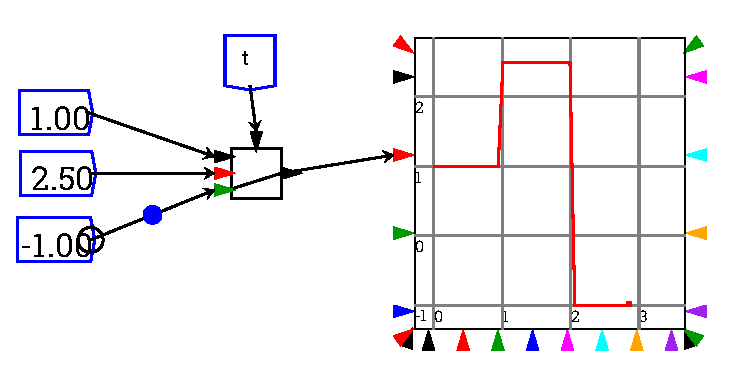
\includegraphics{images/switch.eps}}
{\em An example switch block with 3 cases}
\end{center}

The default switch has two cases, and can be used to implement an
if/then/else construct. However, because the two cases are 0 and 1,
or false and true, a two case switch statement will naturally appear
``upside down'' to how you might think of an if statement. In other
words, it looks like:

\parbox{\textwidth}{
{\tt if not }{\em condition} {\tt then}\\
 \ldots
{\tt else}\\
\ldots
}

You can add or remove cases through the context menu. 

\section{Variables}\label{Variables}\label{Variable:constant}\label{VarConstant}\label{Variable:parameter}
\label{Variable:flow}\label{Variable:integral}\label{Variable:stock}

Variables represent values in a calculation, and come in a number of
varieties:
\begin{description}
\item[Constants] represent an explicit numerical value, and do not
have a name. Their graphical representation shows the actual value of
the constant.
\item[Parameters] are named constants. All instances of a given name
  represent the same value, as with all other named variables, so
  changing the value of one parameter, either through its edit menu,
  or through a slider, will affect all the others of that
  name. Parameters may be \htmlref{imported from a CSV file}{CSV
    import}, which is one way of inserting a tensor into the
  simulation.
\item[Flow variables] have an input port that defines how the value is
to be calculated. Only one flow variable of a given name can have its
input port connected, as they all refer to the same quantity. If no
input ports are connected, then flow variables act just like
parameters.
\item[Integral variables] represent the result of integrating its
input over time  by means of the differential
equation solver. The integrand is represented by the input to an
integral operator that is attached to the integral variable.
\item[Stock variables] are the columns of Godley tables, and represent
the integral over time of the sum of the flow variables making up the
column.
\end{description}

Variables may be converted between types in the variable edit menu,
available from the context menu, subject to certain rules. For example,
a variable whose input is wired anywhere on the canvas cannot be
changed from ``flow''. Stock variables need to be defined in a Godley
table, and so on.

\subsection{Variable names}

Variable names uniquely identify variables. Multiple icons on the
canvas may have the same name --- they all refer to the same
variable. Variable names have scope, which is either local (no initial
`:'), belonging to an outer \htmlref{group}{Group} (indicated by a leading `:' on the
inner group variable, and the outer group variable having no such
leading `:'), or completely global otherwise. You may select a
variable name from a drop down list in the ``name'' combo box, which
makes for an easier way of selecting exactly which variable you want.

\subsection{Initial conditions}\label{var:init}\index{initial conditions}

Variable initial conditions can be defined through the ``init value''
field of the variable edit menu, or in the case of Godley table stock
variables, through the initial condition row of the Godley table. An
initial value can be a simple number, or it can be a multiple of
another named variable (or parameter). In case of symbolic
definitions, it would be possible to set up a circular reference where
the initial value of variable A is defined in terms of the initial
value of variable B, which in turn depends on the intial value of
A. Such a pathological situation is detected when the system is reset.

\subsection{Tensor valued initial conditions}\label{tensor-init}\index{initial conditions|tensor}

There is also a simple functional language, which allows for the
generation of tensor-valued operations. These functions take the form
{\em func}$(n_1,n_2,\ldots,n_r)$ where $r$ is the desired rank, and
$n_1,n_2,$ etc are the dimensions of the tensor. Available
functions include:

\begin{tabular}{|r|l|}
  \hline
  name & description\\\hline
  \verb+one+ & the tensor is filled with `1'\\
  \verb+zero+ & the tensor is filled with `0'\\
  \verb+iota+ & the arithmetic sequence $(0,1,...\prod_in_i)$\\
  \verb+eye+ & diagonal elements filled with `1', offdiagonal `0'\\
  \verb+rand+ & tensor filled with random numbers in the range $[0,1)$\\
  \hline
\end{tabular}
\index{one}\index{zero}\index{iota}\index{eye}\index{rand}

\begin{itemize}
\item \verb+eye+ is equivalent to \verb+one+ for vectors.
\item \verb+rand+ generates different random numbers each time the simulation
  is reset, and uses the clib \verb+rand()+ function.
\end{itemize}


\subsection{Sliders}

From the context menu, one can select a slider to be attached to a
variable, which is a GUI ``knob'' allowing one to control a variable's
initial value, or the value of a parameter or constant. Adjusting the
slider of an integral (or stock) variable while the system is running
actually adjusts the present value of the variable.

Slider parameters are specified in the edit menu: max, min and step
size. A relative slider means that the step size is expressed as a
fraction of max-min.

\subsection{Importing a parameter from a CSV file}\label{CSV import}
\index{CSV|import}\label{Operation:csvImport}

After creating a parameter from the ``Variable'' drop-down in the
``Insert'' menu, right-clicking the parameter and selecting the option
to ``Import CSV'', will open a dialogue box that allows you to select 
a CSV file. Upon selecting the file, a dialog is opened, allowing you to 
specify assorted encoding parameters.

An alternative is to click on the ImportData icon
\buttonIcon{importData.eps}, which will create a new parameter for you
to import the data into.

The dialog looks somewhat like this:

\begin{center}
\resizebox{\textwidth}{!}{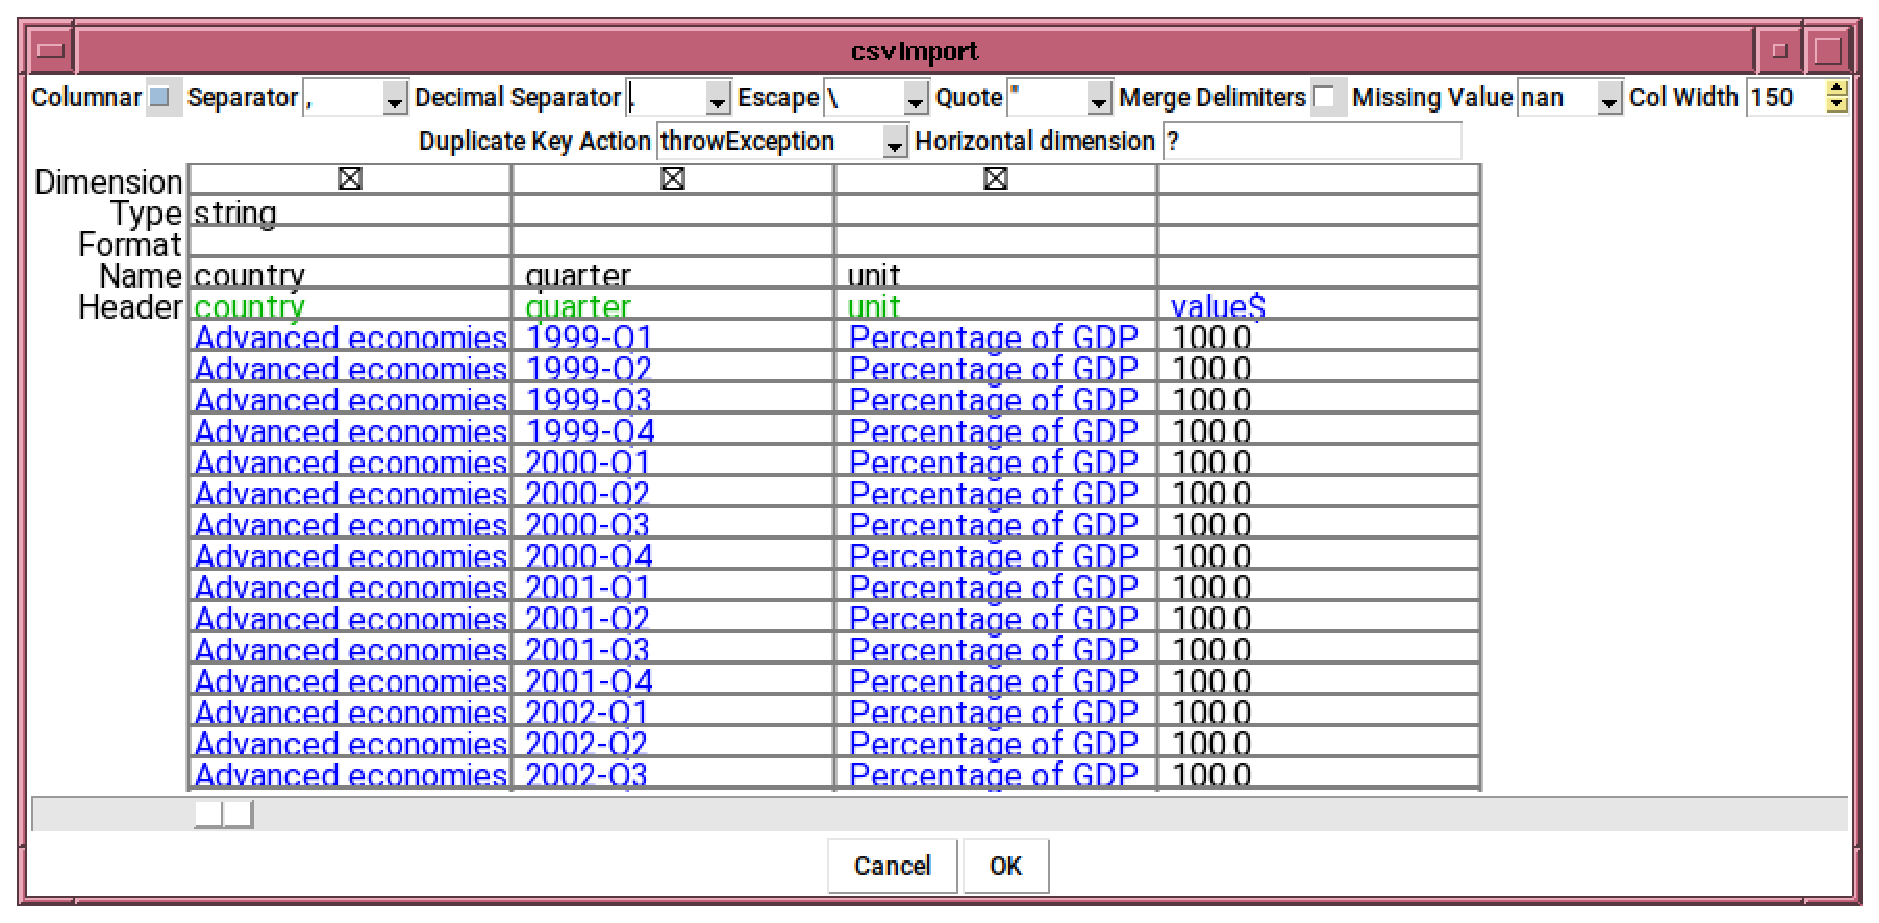
\includegraphics{images/CSVimportDialog.eps}}
\end{center}

Quick instructions:
\begin{itemize}
  \item Data is typically rightmost columns. Click to set the top left
    cell of the data. Columns to the left will be marked as axes.
  \item Select ``axis'' in the Dimension dropdown to include a column
    as an axis. Column data turns blue.
  \item Select ``ignore''  in the Dimension dropdown to exclude a
    column. Column data turns red.
  \item Select ``data''  in the Dimension dropdown to treat a column
    as a data column. Column data turns black.
  \item Select Type for included axis columns. Select one of three
    types:
    \begin{description}
      \item[string] most general type, data treated as is.
      \item[value] value data must be numerical and not quoted, e.g. 1, 2
      \item[time] data must refer to date-time data. Format field
        may be used to control interpretation of this data. Blank
        format assumes data contains year/month/day/hour/minute/second
        separated by some non-numerical character. If fewer than 6
        numerical fields present, smallest units are set to minimum
        value (0 or 1 respectively).
      \end{description}
    \item Click OK button.
    \item Data is imported into the parameter.
    \item You may now need to set units for the imported data field,
      which is located at Edit $\rightarrow$ Dimensions.
    \end{itemize}

In the case shown above, the system has automatically guessed that the data is 3
dimensional, and that the first 3 columns give the axis labels for
each dimension (shown in blue), and the 4th column contains the
data. The first row has been automatically determined to be the first
row of the file --- with the dimension names are shown in green.

In this case, the automatic parsing system has worked things out
correctly, but often times it needs help from the computer user. An
example is as follows:

\begin{center}
\resizebox{\textwidth}{!}{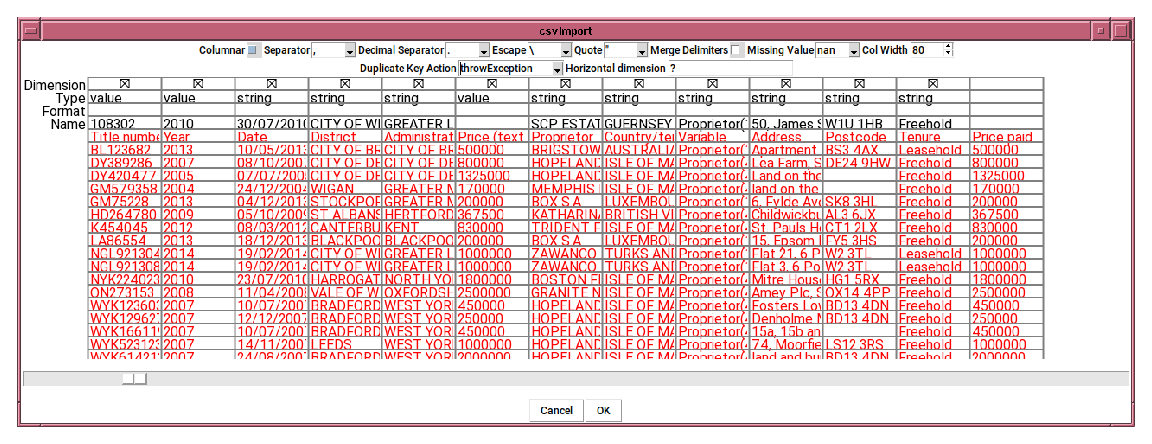
\includegraphics{images/CSVimportDialogFail.eps}}
\end{center}

In this example, Minsky has failed to determine where the data starts,
probably because of the ``Unit'' and ``Frequency'' columns. So the first
thing to do is tell it where the data is located by clicking on the
first cell of the data region. 

\begin{center}
\resizebox{\textwidth}{!}{\includegraphics{images/CSVimportDialogSelectData.eps}}
\end{center}

Note that the data region must lie in the bottom right corner of the
table, so you might need to rearrange the CSV file using a speadsheet
program to ensure this. The ``columnar'' option exists as a way of
ignoring any data to the right of a single data column, useful for the
case where some free form comments are appended to the rows.

Now the axes index labels are rendered in blue, the axes names in
green and the data is in black. In this example, some axes duplicate
others, in effect the data is a planar slice through the hypercube. We
can remove these axes from the data by deselecting the column using
the checkbox in the ``Dimension'' row. The deselected columns are
rendered in red, indicating data that is commented out:

\begin{center}
\resizebox{\textwidth}{!}{\includegraphics{images/CSVimportDialogAxesDeselected.eps}}
\end{center}

In this example, the axis names has not been correctly
inferred. Whilst, one can manually edit the axis names in the ``Name''
line, a quick shortcut is to drag ``Header'' and drop it on ``Name'':

The Date column is current parsed as strings, which not only will be
sorted incorrectly, but even if the data were in a YYYYMMDD format
which is sorted correctly, will not have a uniform temporal
spacing. It is therefore important to parse the Date column as
temporal data, which is achieved by changing the column type to
``time'', and specifying a format string, which follows strftime
conventions with the addition of a quarter specifier (\verb+%Q+).
\index{strftime format specifier}\label{strftime format specifier}

If your temporal data is in the form Y*M*D*H*M*S, where * signifies
any sequence of non-digit characters, and the year, month, day, hour
minutes, second fields are regular integers in that order, then it
suffices to use the blank format string \index{blank strftime
  format}. If some of the fields are missing, eg minutes and seconds,
then they will be filled in with sensible defaults.

\begin{center}
\resizebox{\textwidth}{!}{\includegraphics{images/CSVimportDialogTimeFormat.eps}}
\end{center}

\begin{table}
  \begin{tabular}{|c|l|}
    \hline Code & Description \\\hline
    \%a or \%A &  The name of the day of the week according to the current locale,
                 in abbreviated form or the full name.\\
    \%b or \%B &  The month name according to the current locale,  in  abbreviated
              form or the full name.\\
    \%d & Day of month in range 01 to 31\\
    \%H & Hour in range 0 to 23\\
    \%I & Hour in range 1 to 12\\
    \%m & Month as a decimal number (01 to 12)\\
    \%M & Minute in range 00 to 59\\
    \%Q & Quarter (0=1st January, 1=1st March etc)\\
    \%p & AM or PM\\
    \%s & Number of seconds since epoch (1st January 1970)\\
    \%S & Seconds in range 00 to 59 \\
    \%y & Two digit year YY\\
    \%Y & Four digit year YYYY\\
    \%z & numerical timezone offset\\
    \%Z & Timezone name\\
    \%\% & Literal \% character\\
    \hline
  \end{tabular}
  \caption{Table of strftime codes}
  \label{Strftime code}
\end{table}

Strftime formatted string consists of escape codes (with leading \%
characters). All other characters are treated as matching literally
the characters of the input. So to match a date string of the format
YYYY-MM-DD HH:MM:SS+ZZ (ISO format), use a format string
``\verb|%Y-%m-%d %H:%M:%S+%Z|''. Similarly, for quarterly data
expressed like 1972-Q1, use ``\verb+%Y-Q%Q+''. Note that only \%Y and
\%y can be mixed with \%Q (nothing else makes sense anyway).

Even in the current settings, you may still get a message ``exhausted
memory --- try reducing the rank'', or a similar message about hitting
a 20\% of physical memory threshold. In some cases, ``titles''
and ``addresses'' might be pretty much unique for each record, leading to a
large, but very sparse hypercube. If you remove those columns, as per

\begin{center}
\resizebox{\textwidth}{!}{\includegraphics{images/CSVimportDialogRemoved.eps}}
\end{center}

then you may encounter the ``Duplicate key'' message. In this case, we want
to aggregate over these records, which we can do by setting
``Duplicate Key Action'' to sum. After some additional playing around
with dimensions to aggregate over, we can get the data imported.

\begin{center}
\resizebox{\textwidth}{!}{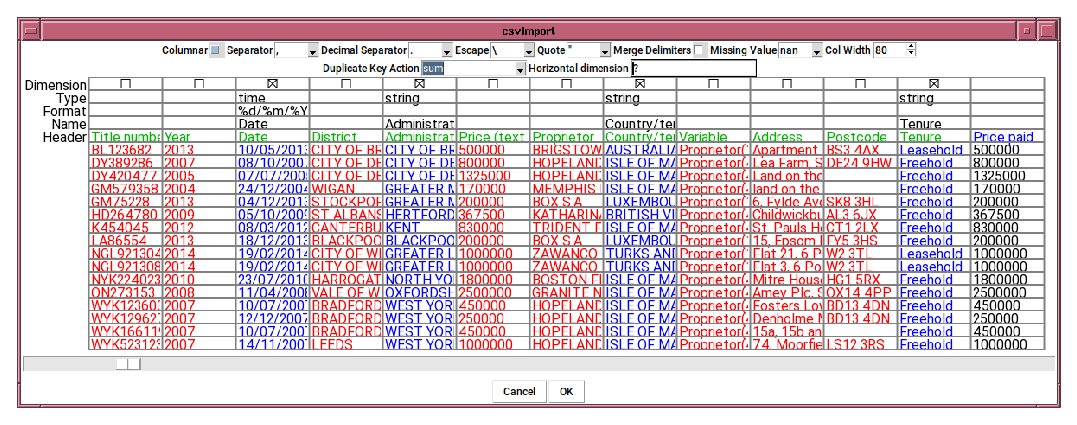
\includegraphics{images/CSVimportDialogFinal.eps}}
\end{center}

\subsection{Duplicate keys}

In a hypercube, data is indexed by a list of indices, collectively
known as a key. The indices may be strings, integers or date/time
values. If more than one value exists in the CSV file for a given key,
Minsky throws a ``Duplicate key'' exception. This exception gives you
the option of writing a report, which is basically a sorted version of
the original CSV file, with the errors listed at the beginning. You
can open this report in a spreadsheet to see if data needs to be
corrected or removed. 

In the case where the data is correct, but there are still duplicate
keys, such as the example in the previous section, the duplicate keys
may be aggregated over by setting the ``Duplicate Key action'' option.

\subsection{Variable Browser}\label{VariableBrowser}

The {\em variable browser} is a popup window that shows all currently
defined variables in the system. This is a convenience toolbar that
allows one to select a variable for insertion into the design canvas,
instead of having to type the new variable's name from scratch.

At the top of the variable browser are some filter checkboxes, that
allow you filter the variables shown by variable type.

\section{Wires}

Wire represent the flow of values from one operation to the next. To
add a wire to the canvas, click on the output port of an operation or
variable (right hand side of the icon in its initial unrotated
orientation), and then drag it towards an input port (on the left hand
side of an unrotated icon). You can't connect an operator to itself
(that would be a loop, which is not allowed, unless passing through an
integral), nor can an input port have more than one wire
attached, with the exception of $+/-$ and $\times/\div$, where the
multiple wires are summed or multiplied, respectively, and similarly max/min.

Wires can be bent by dragging the blue dots (``handles''). Every time
a handle is dragged out of a straight line with its neighbours, new
handles appear on either side. Handles can be removed by
double-clicking on them.

\section{Tensor values}\index{tensors}

Variables may have tensor values, or sets of data. Different tensors
are sorted by rank. For example, a tensor of rank 0 may appear as a
single number, let's refer to it as $x$. A tensor of rank 1 may appear
as a sequence of numbers, let's say $(x x x x)$. Rank 2 means a tensor
appears as a 2D sequence of numbers, for example:

\begin{displaymath}
  \left(
  \begin{array}{ccc}
    x& x& x\\
    x& x& x\\
    x& x& x
  \end{array}
  \right)
\end{displaymath}

A tensor of rank 3 will appear as a three-dimensional cube,
rank 4 as a four-dimensional hypercube, and so on. Two 
ways of getting tensor values into Minsky are via tensor-valued 
initial conditions (\S\ref{tensor-init}), or by importing a CSV 
file into a parameter (\S\ref{CSV import}). Scalar 
operations are extended to operating elementwise over tensors, 
and a number of operations exist for operating on tensors 
(\S\ref{tensor operations}).

When two or more tensors are combined with a binary operation (such 
as addition or multiplication), they must have the same rank. For example,
two tensors of rank 2 can be multiplied together, but a tensor of rank 2 and 
a tensor of rank 3 cannot. They may have differing dimensions, which means
the values within each tensor may not necessarily match up 1-to-1 exactly.
To understand what happens when a given dimension is mismatched requires 
understanding the concept of an x-vector\index{x-vector}\label{x-vector}.

When Minsky is given tensor values, it sorts the values within each tensor
by corresponding dimensions. For example, a rank 2 tensor would have its
values sorted into two sets of data. This data can be in the form of numbers,
dates (time values), or strings. Minsky will then look at cross-sections of the
datasets in order to process the values within. When the dimensions of two
tensors match up, for example two rank 2 tensors, the corresponding
cross-sections of both tensors should also match up. When they don't, a
weighted interpolation of the corresponding values is taken. This involves
using an x-vector. 

An x-vector is a vector of real values, strings or date/time values. 
If no x-vector is explicitly provided, then implicitly it consists of the the values
$(0,\ldots,n_i-1)$, where $n_i$ is the dimension size of axis $i$
of the tensor.

For example, if the first tensor consists of three elements $(x_0, x_1, x_2)$
and the second consist of a number of different elements that roughly
correspond to the same three elements, these can be added together.
The x-vector starts with the first tensor's value of $(x_0)$ and looks for a
matching value in the second tensor. If it can't find a direct match, it will
search for nearby values which roughly correspond. It can then take those
values and interpolate the corresponding value based on where in the tensor
it appears. This is weighted, so say there are four values nearby, the program
will average those out and find where a value in the middle of those four
values would appear, and what that hypothetical value would be. To take
another example:

Suppose the first tensor was a vector $(x_0,x_1)$ and had an
x-vector (1,3) and the second tensor $(y_0,y_1,y_2)$ had an x-vector
(0,2,3), then the resulting tensor will be $(x_0+0.5(y_0+y_1),
x_1+y_2)$. If the x-vector were date/time data, then the tensor values
will be interpolated according to the actual time values. If the first
tensor's x-vector value lies outside the second tensor's x-vector,
then it doesn't result in a value being included in the output. The
resultant x-vector's range of values is the intersection of input
tensors' x-vector ranges.

If both tensor had string x-vectors, then the resultant tensor will
only have values where both input tensors have the same string value
in their x-vectors. In the above case, where the x-vectors were
('1','3') and ('0','2','3') the resulting tensor will be the scalar $x_1+y_2$.

It goes without saying that the type of the x-vector for each axis
must also match.

\section{Groups}\label{Group}

Grouping gives the capability to create reusable modules, or subroutines that
can dramatically simplify more complicated systems. Groups may be
created in the following ways:
\begin{itemize}
\item by lassoing a number of items to select them, then selecting
``group'' from the canvas context menu, or the edit menu.
\item by pasting the selection. You may ``ungroup'' the group from the
context menu if you don't desire the result of the paste to be a group.
\item by copying another group
\item by inserting a Minsky file as a group
\end{itemize}

Zooming in on a group allows you see and edit its contents. Groups may
be nested heirarchically, which gives an excellent way of zooming in
to see the detail of a model, or zooming out to get an overview of
it. The group context menu item ``Zoom to display'' zooms the canvas
in just enough for the group's contents to be visible.

You may also select ``Open in canvas'' from the context menu. This
replaces the current canvas contents with the contents of the group,
allowing you to edit the contents of the group directly without the
distractions of the rest of the model. Select ``Open master group'' to
return to the top level group occupying the canvas.

Around the edges of a group are input or output variables, which allow
one to parameterise the group. One can drag a variable and dock it in
the I/O area to create a new input or output for the group.

When creating a group, or dragging a variable or operation into or out
of a group, if a wire ends up crossing the group boundary, a new
temporary variable is added as an I/O variable.

Variable names within groups are locally scoped to that group. That
means that a variable of the same name outside the group refers to a
different entity completely. One can refer to variables outside the
current scope by prepending the variable name with a `:'. This refers
to a local variable within an outer scope, going all the way to global
scope if no such variable exists. In this way, two groups can share
a variable reference to a variable by using the `:' prefix, and you
can limit the scope of the shared variable by placing a local variable
of the same name in an outer group that both groups are contain within.

A group can also be exported to a file from the context menu.
This allows you to build up a library of building blocks. There is a
github project ``minsky-models'' allowing people to publish their
building blocks and models for others to use. In the future, we hope
to integrate Minsky with this github repository, allowing even more
seamless sharing of models.

\section{Plot widget}
\label{PlotWidget}

A plot widget embeds a dynamic plot into the canvas. Around the
outside of the plot are a number of input ports that can be wired.

\begin{center}
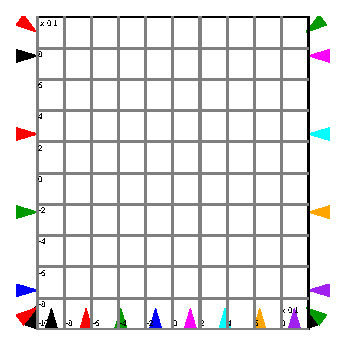
\includegraphics{images/plotWidget.eps}
\end{center}

\begin{description}
\item[left hand edge] Up to 4 quantities can be plotted on the graph
  simultaneously, with line colour given by the colour of the input
  port
\item[right hand edge] Another 4 quantities can be added to the
  plot. These are shown on a different scale to the left hand inputs,
  allowing very different magnitudes to be compared on the one plot.
\item[bottom edge] Quantities controlling the $x$-coordinates of the
  curves. The colours match up with the colour of the pen being
  controlled.

\begin{center}
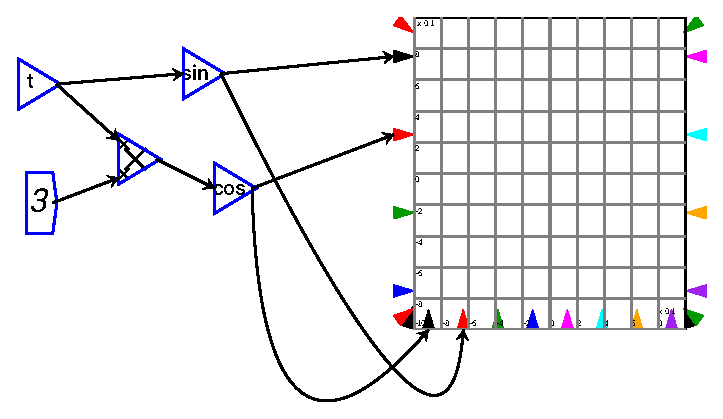
\includegraphics{images/plotLissajous.eps}
\end{center}

  If only one bottom port is connected, then that controls all pens
  simultaneously, and if no ports are connected, then the simulation
  time is used to provide the $x$ coordinates
\item[corners] Corner ports control the scale. You can wire up
  variables controlling minimum and maximum of the $x$, $y$ and right hand
  $y$ axes. If left unwired, the scales are determined automatically
  from the data. This can be used, for example, to implement a sliding
  window graph

\begin{center}
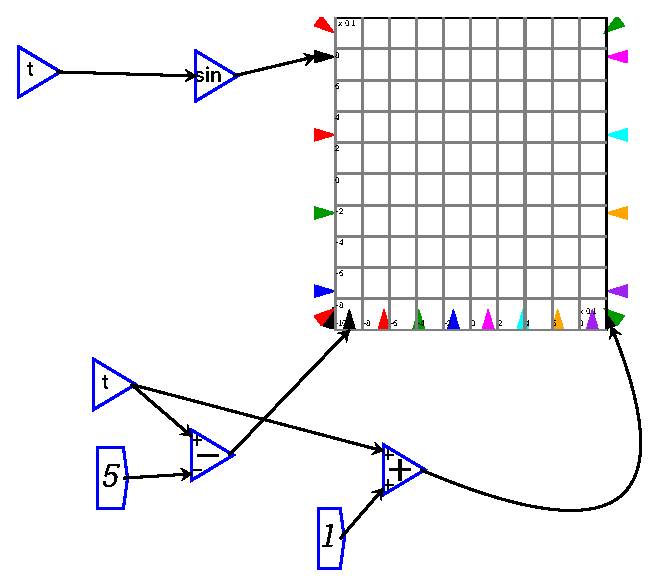
\includegraphics{images/plotSlidingWindow.eps}
\end{center}
\end{description}

\section{Sheet Widget}
 \label{Sheet} The Sheet widget displays input data as a
 number, rather than as a 2D graph, as in the case of the plot widget.
 To use the Sheet widget, simply wire a variable or other item on your
 canvas to the left-hand side of the sheet widget box. This will diplay
 the input data as a number. Note that only one wire can be connected to
 a sheet, as the sheet can only display a single input value.
 
 The sheet widget can also display rank 0, 1 and rank 2 tensors. These ranks are
 single values, a string of values, or a 2D matrix of values, respectively.
 For example, if you create a parameter, and set the initial condition to rand(3,5)
 (for reference, see section (\S\ref{tensor-init}) ), you can wire that into a sheet.
 The sheet will then diplay the data in a grid display within the widget box.

\section{Note Widget}
 \label{Notes}\label{Item} Notes allow arbitrary text to be
placed on the canvas for explanatory purposes. Anything that can be
entered on the keyboard can be placed here, including unicode
characters, and LaTeX formatting is supported. A note
widget, like all canvas items, allow short additional tooltips to be
specified. It is also possible to annotate an ordinary block with some text
that is accessed through the edit menu, or as a tooltip.

\section{Godley Tables}\label{godley}\label{GodleyIcon}

Godley tables describes sets of financial flows from the point of view
of a particular economic agent, such as a bank. The columns of the
table represent accounts (possibly aggregated), which are treated as
integration variables by the system. Accounts may be assets,
liabilities or equities. Assets may appear as liabilities in another
agent's Godley table, and vice versa, with the sense of the financial
flows treated oppositely (a credit flow increasing the asset of one
entity will appear as a debit flow, increasing the value of a
liability). Transfers between accounts should satisfy the {\em
  accounting equation}\index{accounting equation}
(Assets-Liabilities-Equities = 0). So if the transfer is between an
asset and a liability, then it should appear with the same sign (both
positive or both negative), otherwise between two accounts of the same
type, or between a liability and an equity, the terms should have
opposite signs.

Instead of signed flows, one can optionally use CR and DR prefixes, as
specified in the options panel. Each row of the table should have have
one CR entry, and one DR entry. The row sum column should be zero if
it is done correctly.

The first row specifies the stock variables, after which follow the
flow rows. Usually, the row marked ``Initial Conditions'' comes next,
but may be placed in any position. These specify the initial
conditions of the stock variables, and may refer to a multiple of
another variable, just like the \htmlref{initial condition
field}{var:init}, or just be a numerical value.

Finally come the flows. The first column is a simple textual label
(the phrase ``Initial Conditions'', regardless of capitalisation, is a
reserved phrase for setting stock variable initial conditions)
identifying the flow. The flows themselves are written as a numerical
multiplier times a flow variable. For example, if you wanted to transfer
an amount between the asset and liability column, you might write
``Amount" in both columns, which would satisfy the equation A-L-E=0.
It would also be possible to write ``2Amount" in the asset column, 
along with ``Amount" in both the Liability and Equity columns. This would
still satisfy A-L-E=0.

The Godley table also shows the value of the entered variable, displayed within the table.
For example, if you set ``Amount" to equal the value of system time, on opening
the Godley table, wherever you entered ``Amount" in the table the cell would show
``Amount = 0.00" if the system time was set to 0.00. This provides a helpful
tool for displaying the value of the variable at that point in the simulation.
This feature can be enabled or disabled in the preferences panel.

\section{Context Menu}

All canvas items have a context menu, which allow a variety of
operations to be applied to the canvas item. Common context menu items
are explained here:
\begin{description}
\item[Help] bring up context specific help for the item
\item[Description] Attach an annotation to the item. This is only
visible by selecting the description item from the context menu,
although whatever is set as the ``Short Description'' will also appear
as a tooltip whenever the mouse hovers over the item.
\item[Port values] When running a simulation, you can drill down into
the actual values at the input and output ports of the variable or
operation, which is a useful aid for debugging models.
\item[Edit] set or query various attributes of an item. This function
can also be accessed by double clicking on the item. (Plot widgets
behave slightly differently).
\item[Copy] Creates a copy of an item, retaining the same attributes
of the original. This is very useful for creating copies of the same
variable to reduce the amount of overlapping wiring (aka ``rats nest")
in a model.
\item[Flip] actually rotates an object through $180^\circ$. You can
specify aribtrary rotations of objects through the edit menu.
\item[Raise/Lower] Raise and lower the canvas items relative to each
other. You may need to do this if a large item such as a Godley table
or plot is obscuring a wire, making it hard to access the wire's
context menu or handles,
\item[Browse object] gives a low level drilldown of the internal C++
object this canvas item represents. It is perhaps more of interest to
developers. 
\item[Delete] delete the object.
\end{description}

Item specific context menu items:
\begin{description}
\item[variables, parameters and constants]\mbox{}
\begin{description}
\item[Slider] add a slider control to a variable. This is most
effective for controlling parameters and constants, but can also be
used to control inputless variables.
\item[Add integral] attach an integration operation, and convert the
variable into an integral type
\end{description}
\item[integrals]\mbox{}
\begin{description}
\item[Copy Var] copy just the integration variable, not the
integration operation
\item[Toggle Var Binding] Normally, integrals are tightly bound to their
variables. By toggling the binding, the integral icon can then be
moved independently of the variable it is bound to. 
\end{description}
\item[Godley tables]\mbox{}
\begin{description}
\item[Open Godley Table] opens a spreadsheet to allow financial flows
defining the Godley table to be entered or modified.
\item[Resize Godley Table] allows the icon to be resized.
\item[Edit/Copy var] allows individual stock and flow variables to be
copied or edited.
\item[Export to file] export table contents as either CSV data, or as a LaTeX
table, for import into other software.
\end{description}

\item[Groups]\mbox{}
\begin{description}
\item[Zoom to Display] Zoom the canvas sufficiently to see the
contents of the group.
\item[Resize] Resize the group icon on the canvas.
\item[Save group as] Save the group in it's own Minsky file.
\item[Flip contents] Rotate each item within the group by 180$^\circ$
\item[Ungroup] Ungroup the group, leaving it's contents as icons on
the canvas.
\item[contentBounds] Draws a box on the canvas indicating the smallest
bounding box containing the group items.
\end{description}


\item[Plot Widgets]\mbox{}
\begin{description}
\item[Expand]
By double-clicking, or selecting ``Expand'' from the context menu, a
popup window is created of the plot, which can be used examine the
plotting in more detail.

\item[Resize] Allows you to resize the plot icon on the canvas
\item[Options] Customize the plot by adding a title, axes labels and
  control the number of axis ticks and grid lines on the detailed
  plot. You can also add a legend, which is populated from the names
  of variables attached to the plot.
\end{description}

\end{description}

\section{Canvas background}

The canvas is not simply an inert place for the canvas items to
exist. There is also a background context menu, giving access to the
edit menu functionality such as cut/copy/paste, and also keyboard entry.

The following keystrokes insert an operation

\begin{tabular}{rl}
  \verb-+- & add\\
  \verb+-+ & subtract \\
  \verb+*+ & multiply\\
  \verb++/ & divide\\
  \verb+^+ & pow\\
  \verb+%+ & percent operator\\
  \verb+&+ & integral\\
  \verb+=+ & Godley table\\
  \verb+@+ & plot\\
  \verb+#+ & start a text comment, finish with return\\
\end{tabular}

Typing any other character, then return will insert an operation (if
the name matches), or otherwise a variable with that name.

\section{Dimensional Analysis}

Dimensional analysis is the idea of attaching units of measurement
(eg metre or second) to the quantities being computed. It provides an 
additional constraint that the system must satisfy, reducing the chance 
of wiring errors. Two different units being added together will throw up 
an error - you cannot add 2 metres to 3 kilograms. But it should be 
possible add 2 metres to 3 feet, and get the correct answer. You may need 
to explicitly add a multiply operation to convert from one unit to another,
for example, dividing the 3 feet by 3.281 before adding it to the 2 metres,
providing a total of 2.914 meters.

\textbf{Using Dimensional Analysis in Minsky}

To attach units to quantities in Minsky, you use the units field of the 
variable/parameters/constants edit dialog box. Each word typed in this box 
describes a separate unit. ``\^{}'' followed by an integer is used to 
represent a power. Finally, a single ``/'' indicates that the following units 
are on the denominator, dividing the first set of units by the second. So 
to represent the unit of acceleration, you can equivalently type all of the following:

\begin{itemize}
  \item \verb+m/s^2+
  \item \verb+m/s s+
  \item \verb+m/s^-2+
\end{itemize}

Or spelling it out in full:

\begin{itemize}
  \item \verb+metre/second^2+
  \item \verb+metre second^-2+
  \item \verb+metre / second second+
\end{itemize}

Note that metre and m are distinctly different units in Minsky.

Note -- setting the time dimension is done in the \hyperref[ref]{simulation menu}{simulation menu}{}{RungeKutta}

Consider the network introduced in the \hyperref[ref]{New to System Dynamics}{New to System Dynamics}{}{intro:new}
section of the Minsky manual. For GDP, one could enter \$/year for the units. Labor 
Productivity should be expressed in terms of \$ per person year. If the system
does not accept \$/person year, you can enter this as \verb+$ person^-1 year^-1+. 
Finally, Population has units of person. Press reset, and the Workers variable 
automatically has units of person, and EmpRate is dimensionless.

All function objects require dimensionless inputs. You can use dimensional 
analysis to prevent incorrectly feeding a degree measurement into a sin, by 
requiring them to be multiplied by a radiansPerDegree parameter.

\section{Bookmarks}

Bookmarks are a useful feature for saving the current position and
zoom of the canvas, to be able to come back to that part of the canvas
later. This helps managing more complicated models.  To create a new
bookmark, click on the ``Bookmark'' tab in the top left-hand corner
(in-between ``Edit'' and ``Insert'') and select ``Bookmark this
position''. The program will provide a dialogue box to enter in a name
for the new bookmark. After creating the bookmark, all user-created
bookmarks can be seen in the Bookmarks menu. To delete a bookmark,
simply select ``Delete'' from the Bookmarks menu and select the
desired bookmark. To open an existing bookmark, select one from the
menu.

\section{Ravel}\label{Ravel}\label{Lock}

Ravel is a skunkworks project enabling the interactive manipulation of
multidimensional datacubes. This is a commercial technology, and you
will need a license to use the software, as well as a copy of the
Ravel plugin. This is still under active development, but you can read
some more about it at \htmladdnormallink{Ravelation}{https://ravelation.hpcoders.com.au}.

The Lock widget is used to fix the output of a Ravel at a particular
point in time, making it easy to compare two different ravel settings.

\chapter{User defined functions}\label{ExprTk}

{\em Much of this chapter is exerpted from \htmladdnormallink{exprtk's
read.txt
file}{https://github.com/ArashPartow/exprtk/blob/master/readme.txt}}

\section{Introduction}
The \htmladdnormallink{C++ Mathematical Expression  Toolkit Library (ExprTk)}{https://www.partow.net/programming/exprtk/index.html} is  a simple
to  use,   easy  to   integrate  and   extremely  efficient   run-time
mathematical  expression parsing  and evaluation  engine. The  parsing
engine  supports numerous  forms  of  functional and  logic processing
semantics and is easily extensible.

With Minsky's user defined functions, expressions can refer to Minsky
variables accessible from the current scope (ie local Minsky variables
will hide global variables), and also parameters declared as part of
the function name. One can also call other user defined functions,
which is the only way a user defined function with more than 2
parameters can be used. For 0-2 parameters, user defined functions can
be wired into a Minsky computation.

ExprTk identifiers (such as variable names and function names) consist
of alphanumeric characters plus '\_' and '.'. They must start with a
letter. Minsky is reserving the underscore and full stop to act as an
escape sequence, in order to refer to the full range of possible
Minsky variable identifiers, including all unicode characters. This
section will be updated once that feature is in place --- for now,
please avoid using those characters in identifiers.

\section{Capabilities}
The  ExprTk expression  evaluator supports  the following  fundamental
arithmetic operations, functions and processes:

\begin{description}
 \item[Types:]           Scalar, Vector, String

 \item[Basic operators:] \verb'+, -, *, /, %, ^'

 \item[Assignment:]      \verb':=, +=, -=, *=, /=, %='

 \item[Equalities \& Inequalities:]    \verb'=, ==, <>, !=, <, <=, >, >='

 \item[Logic operators:] and, mand, mor, nand, nor, not, or, shl, shr,
                       xnor, xor, true, false

 \item[Functions:]       abs, avg, ceil, clamp, equal, erf, erfc,  exp,
                       expm1, floor, frac,  log, log10, log1p,  log2,
                       logn,  max,  min,  mul,  ncdf,  nequal,  root,
                       round, roundn, sgn, sqrt, sum, swap, trunc

 \item[Trigonometry:]    acos, acosh, asin, asinh, atan, atanh,  atan2,
                       cos,  cosh, cot,  csc, sec,  sin, sinc,  sinh,
                       tan, tanh, hypot, rad2deg, deg2grad,  deg2rad,
                       grad2deg

 \item[Control structures:]      if-then-else, ternary conditional, switch-case,
                       return-statement

 \item[Loop statements:] while, for, repeat-until, break, continue

 \item[String processing:]      in, like, ilike, concatenation

 \item[Optimisations:]   constant-folding, simple strength reduction and
                       dead code elimination

 \item[Calculus:]        numerical integration and differentiation

\end{description}

\section{Example expressions}
The following is  a short listing  of infix format  based mathematical
expressions that can be parsed and evaluated using the ExprTk library.

\begin{itemize}
  \item \verb'sqrt(1 - (3 / x^2))'
  \item \verb'clamp(-1, sin(2 * pi * x) + cos(y / 2 * pi), +1)'
  \item \verb'sin(2.34e-3 * x)'
  \item \verb'if(((x[2] + 2) == 3) and ((y + 5) <= 9),1 + w, 2 / z)'
  \item \verb'inrange(-2,m,+2) == if(({-2 <= m} and [m <= +2]),1,0)'
  \item \verb'({1/1}*[1/2]+(1/3))-{1/4}^[1/5]+(1/6)-({1/7}+[1/8]*(1/9))'
  \item \verb'a * exp(2.2 / 3.3 * t) + c'
  \item \verb'z := x + sin(2.567 * pi / y)'
  \item \verb'u := 2.123 * {pi * z} / (w := x + cos(y / pi))'
  \item \verb'2x + 3y + 4z + 5w == 2 * x + 3 * y + 4 * z + 5 * w'
  \item \verb'3(x + y) / 2.9 + 1.234e+12 == 3 * (x + y) / 2.9 + 1.234e+12'
  \item \verb'(x + y)3.3 + 1 / 4.5 == [x + y] * 3.3 + 1 / 4.5'
  \item \verb'(x + y[i])z + 1.1 / 2.7 == (x + y[i]) * z + 1.1 / 2.7'
  \item \verb'(sin(x / pi) cos(2y) + 1) == (sin(x / pi) * cos(2 * y) + 1)'
  \item \verb'75x^17 + 25.1x^5 - 35x^4 - 15.2x^3 + 40x^2 - 15.3x + 1'
  \item \verb'(avg(x,y) <= x + y ? x - y : x * y) + 2.345 * pi / x'
  \item \verb'while (x <= 100) { x -= 1; }'
  \item \verb"x <= 'abc123' and (y in 'AString') or ('1x2y3z' != z)"
  \item \verb"((x + 'abc') like '*123*') or ('a123b' ilike y)"
  \item \verb'sgn(+1.2^3.4z / -5.6y) <= {-7.8^9 / -10.11x }'
\end{itemize}

\section{Copyright notice}
Free  use  of  the  C++  Mathematical  Expression  Toolkit  Library is
permitted under the guidelines and in accordance with the most current
version of the \htmladdnormallink{MIT License}{http://www.opensource.org/licenses/MIT}


\section{Built-in operations \& functions}

\subsection{Arithmetic \& Assignment Operators}

\begin{tabular}{|c|p{0.8\textwidth}|}
\hline
OPERATOR & DEFINITION \\
\hline
\verb'+' &  Addition between x and y.  (eg: \verb'x + y')\\
\verb'-'& Subtraction between x and y.  (eg: \verb'x - y')\\
\verb'*'&   Multiplication between x and y.  (eg: \verb'x * y')\\
\verb'/'& Division between x and y.  (eg: \verb'x / y')\\
\verb'%'& Modulus of x with respect to y.  (eg: \verb'x % y')\\
\verb'^'& $x^y$.  (eg: \verb'x ^ y')\\
\verb':='& Assign the value of x to y. Where y is either a variable
 or vector type.  (eg: \verb'y := x')\\
\verb'+='&Increment x by the value of the expression on the right 
hand side. Where x is either a variable or vector type. 
(eg: \verb'x += abs(y - z)')\\
\verb'-='&  Decrement x by the value of the expression on the right 
hand side. Where x is either a variable or vector type. 
(eg: \verb'x[i] -= abs(y + z)')\\
\verb'*='& Assign the multiplication of x by the value of the 
 expression on the righthand side to x. Where x is either
 a variable or vector type. (eg: \verb'x *= abs(y / z)')\\
\verb'/='& Assign the division of x by the value of the expression
on the right-hand side to x. Where x is either a  variable or vector
type.  (eg: \verb'x[i + j] /= abs(y * z)')\\
\verb'%='& Assign x modulo the value of the expression on the right
hand side to x. Where x is either a variable or vector type.  (eg:
\verb'x[2] %= y ^ 2')\\
\hline
\end{tabular}

\subsection{Equalities \& Inequalities}

\begin{tabular}{|c|p{0.8\textwidth}|}
\hline
OPERATOR & DEFINITION\\
\hline
\verb'==' or \verb'=' & True only if x is strictly equal to y. (eg: \verb'x == y')\\
\verb'<>' or \verb'!='& True only if x does not equal y. (eg: \verb'x <> y' or \verb'x != y')\\
\verb'<'& True only if x is less than y. (eg: \verb'x < y')\\
\verb'<='& True only if x is less than or equal to y. (eg: \verb'x <= y')\\
\verb'>'& True only if x is greater than y. (eg: \verb'x > y'\\
\verb'>='& True only if x greater than or equal to y. (eg: \verb'x >= y')\\
\hline
\end{tabular}

\subsection{Boolean Operations}

\begin{tabular}{|c|p{0.8\textwidth}|}
\hline
OPERATOR& DEFINITION\\
\hline
\verb'true'& True state or any value other than zero (typically 1).\\
\verb'false'& False state, value of exactly zero.\\
\verb'and'& Logical AND, True only if x and y are both true. (eg: \verb'x and y')\\
\verb'mand'& Multi-input logical AND, True only if all inputs are true. Left to right short-circuiting of expressions. (eg: \verb'mand(x > y, z < w, u or v, w and x)')\\
\verb'mor'& Multi-input logical OR, True if at least one of the inputs
are true. Left to right short-circuiting of expressions.  (eg:
\verb'mor(x > y, z < w, u or v, w and x)')\\
\verb'nand'& Logical NAND, True only if either x or y is false. (eg: \verb'x nand y')\\
\verb'nor'& Logical NOR, True only if the result of x or y is false (eg: \verb'x nor y')\\
\verb'not'& Logical NOT, Negate the logical sense of the input. (eg: \verb'not(x and y) == x nand y')\\
\verb'or'& Logical OR, True if either x or y is true. (eg: \verb'x or y') \\
\verb'xor'& Logical XOR, True only if the logical states of x and y differ.  (eg: \verb'x xor y')\\
\verb'xnor'& Logical XNOR, True iff the biconditional of x and y is
satisfied.  (eg: \verb'x xnor y')\\
\verb'&'& Similar to AND but with left to right expression short circuiting optimisation.  (eg: \verb'(x & y) == (y and x)')\\
\verb'|'& Similar to OR but with left to right expression short
circuiting optimisation.  (eg: \verb'(x | y) == (y or x)')\\
\hline
\end{tabular}

\subsection{General Purpose Functions}

\begin{tabular}{|c|p{0.8\textwidth}|}
\hline
FUNCTION & DEFINITION\\
\hline
\verb'abs'& Absolute value of x.  (eg: \verb'abs(x)')\\
\verb'avg'& Average of all the inputs. (eg: \verb'avg(x,y,z,w,u,v) == (x + y + z + w + u + v) / 6')\\
\verb'ceil'& Smallest integer that is greater than or equal to x.\\
\verb'clamp'& Clamp x in range between r0 and r1, where r0 < r1. (eg:
\verb'clamp(r0,x,r1)')\\
\verb'equal'& Equality test between x and y using normalised epsilon\\
\verb'erf'& Error function of x.  (eg: \verb'erf(x)')\\
\verb'erfc'& Complimentary error function of x.  (eg: \verb'erfc(x)')\\
\verb'exp'& $e^x$  (eg: \verb'exp(x)')\\
\verb'expm1'& $e^{x-1}$ where $x$ is very small. (eg: \verb'expm1(x)')\\ 
\verb'floor'& Largest integer that is less than or equal to x. (eg: \verb'floor(x)')\\
\verb'frac'& Fractional portion of x.  (eg: \verb'frac(x)')\\
\verb'hypot'& $\sqrt{x^2+y^2}$ (eg: \verb'hypot(x,y) = sqrt(x*x + y*y)')\\
\verb'iclamp'& Inverse-clamp x outside of the range r0 and r1. Where
r0 < r1. If x is within the range it will snap to the closest
bound. (eg: \verb'iclamp(r0,x,r1)'
\begin{math}
=\left\{\begin{array}{ccc}
r0 & \mathrm{if} & x\le r0\\
x & \mathrm{if} & r0\le x \le r1\\
r1 & \mathrm{if} & x\ge r1\\
\end{array}\right.
\end{math}
)\\
\verb'inrange'&  In-range returns 'true' when $x$ is within the range $[r_0,r_1]$. Where $r_0 < r_1$.  (eg: \verb'inrange(r0,x,r1)')\\
\verb'log'& Natural logarithm $\ln x$.  (eg: \verb'log(x)')\\
\verb'log10'& $\log_{10}x$.  (eg: \verb'log10(x)')\\
\verb'log1p'& $\ln (1+x)$, where $x$ is very small. (eg: \verb'log1p(x)')\\
\verb'log2'& $\log_2x$.  (eg: \verb'log2(x)')\\
\verb'logn'& $\log_nx$, where $n$ is a positive integer. (eg: \verb'logn(x,8)')\\
\verb'max'& Largest value of all the inputs. (eg: \verb'max(x,y,z,w,u,v)')\\
\verb'min'& Smallest value of all the inputs. (eg: \verb'min(x,y,z,w,u)')\\
\verb'mul'& Product of all the inputs. (eg: \verb'mul(x,y,z,w,u,v,t) == (x * y * z * w * u * v * t)') \\
\verb'ncdf'& Normal cumulative distribution function.  (eg: \verb'ncdf(x)')\\
\verb'nequal'& Not-equal test between $x$ and $y$ using normalised epsilon\\
\verb'pow'& $x^y$.  (eg: \verb'pow(x,y) == x ^ y')\\
\verb'root'&  $\sqrt[n]{x}$, where $n$ is a positive integer. (eg: \verb'root(x,3) == x^(1/3)')\\
\verb'round'& Round $x$ to the nearest integer.  (eg: \verb'round(x)')\\
\verb'roundn'& Round $x$ to $n$ decimal places  (eg: \verb'roundn(x,3)')
 where $n > 0$ is an integer. (eg: \verb'roundn(1.2345678,4) == 1.2346')\\\verb'sgn'& Sign of $x$, $-1$ where $x < 0$, +1 where $x > 0$, else zero.
 (eg: \verb'sgn(x)')\\
\verb'sqrt'& $\sqrt{x}$, where $x >= 0$.  (eg: \verb'sqrt(x)')\\ 
\verb'sum'& Sum of all the inputs. (eg: \verb'sum(x,y,z,w,u,v,t) == (x + y + z + w + u + v + t)')\\
\verb'swap'\\\verb'<=>'& Swap the values of the variables x and y and return the current value of y.  (eg: \verb'swap(x,y)' or \verb'x <=> y')\\
\verb'trunc'& Integer portion of x.  (eg: \verb'trunc(x)')\\
\hline
\end{tabular}

\subsection{Trigonometry Functions}

\begin{tabular}{|c|p{0.8\textwidth}|}
\hline
FUNCTION & DEFINITION\\
\hline
\verb'acos'& Arc cosine of x expressed in radians. Interval $[-1,+1]$
(eg: \verb'acos(x)')\\
\verb'acosh'& Inverse hyperbolic cosine of x expressed in radians. (eg: \verb'acosh(x)')\\
\verb'asin'& Arc sine of x expressed in radians. Interval $[-1,+1]$ (eg: \verb'asin(x)')\\
\verb'asinh'& Inverse hyperbolic sine of x expressed in radians. (eg:
\verb'asinh(x)')\\
\verb'atan'& Arc tangent of x expressed in radians. Interval $[-1,+1]$
(eg: \verb'atan(x)')\\
\verb'atan2'& Arc tangent of $(x / y)$ expressed in
radians. $[-\pi,+\pi]$ (eg: \verb'atan2(x,y)')\\
\verb'atanh'& Inverse hyperbolic tangent of $x$ expressed in radians. (eg: \verb'atanh(x)')\\
\verb'cos'& Cosine of $x$.  (eg: \verb'cos(x)')\\
\verb'cosh'& Hyperbolic cosine of $x$.  (eg: \verb'cosh(x)')\\
\verb'cot'& Cotangent of $x$.  (eg: \verb'cot(x)')\\
\verb'csc'& Cosecant of $x$.  (eg: \verb'csc(x)')\\ 
\verb'sec'& Secant of $x$.  (eg: \verb'sec(x)')\\
\verb'sin'& Sine of $x$.  (eg: \verb'sin(x)')\\
\verb'sinc'& Sine cardinal of $x$.  (eg: \verb'sinc(x)')\\
\verb'sinh'& Hyperbolic sine of $x$.  (eg: \verb'sinh(x)')\\
\verb'tan'& Tangent of $x$.  (eg: \verb'tan(x)')\\
\verb'tanh'& Hyperbolic tangent of $x$.  (eg: \verb'tanh(x)')\\ 
\verb'deg2rad'& Convert $x$ from degrees to radians.  (eg: \verb'deg2rad(x)')\\
\verb'deg2grad'& Convert $x$ from degrees to gradians.  (eg: \verb'deg2grad(x)')\\
\verb'rad2deg'& Convert $x$ from radians to degrees.  (eg: \verb'rad2deg(x)')\\
\verb'grad2deg'& Convert $x$ from gradians to degrees.  (eg: \verb'grad2deg(x)')\\
\hline
\end{tabular}

\subsection{String Processing}
\begin{tabular}{|c|p{0.8\textwidth}|}
\hline
FUNCTION& DEFINITION\\
\verb'=' , \verb'==', \verb'!=', \verb'<>', \verb'<=', \verb'>=', \verb'<' , \verb'>'& All common equality/inequality operators are applicable to strings and are applied in a case sensitive manner. In the following example x, y and z are of type string. (eg: \verb"not((x <= 'AbC') and ('1x2y3z' <> y)) or (z == x)")\\
\verb'in'& True only if $x$ is a substring of $y$. (eg: \verb'x in y' or \verb"'abc' in 'abcdefgh'")\\
\verb'like'& True only if the string x matches the pattern y.  Available wildcard characters are `*' and `?' denoting  zero or more and zero or one matches respectively.   (eg: \verb'x like y' or \verb"'abcdefgh' like 'a?d*h'")\\ 
\verb'ilike'& True only if the string x matches the pattern y in a case insensitive manner. Available wildcard characters are '*' and '?' denoting zero or more and zero or one  matches respectively. (eg: \verb'x ilike y' or \verb"'a1B2c3D4e5F6g7H' ilike 'a?d*h'")\\
\verb'[r0:r1]'& The closed interval $[r0,r1]$ of the specified string.
eg: Given a string x with a value of 'abcdefgh' then:
\begin{enumerate}
\item \verb"x[1:4] == 'bcde'"
\item \verb"x[ :5] == x[:10 / 2] == 'abcdef'"
\item \verb"x[2 + 1: ] == x[3:] =='defgh'"
\item \verb"x[ : ] == x[:] == 'abcdefgh'"
\item \verb"x[4/2:3+2] == x[2:5] == 'cdef'"
\end{enumerate}
 Note: Both r0 and r1 are assumed to be integers, where r0 <= r1. They
 may also be the result of an expression, in the event they have
 fractional components truncation will be performed. (eg: $1.67
                \rightarrow 1$)\\
  %begin{latexonly}
  \hline
\end{tabular}

\begin{tabular}{|c|p{0.8\textwidth}|}
\hline
FUNCTION& DEFINITION\\
  \hline
  %end{latexonly}
\verb':='& Assign the value of x to y. Where y is a mutable string  or
 string range and x is either a string or a string  range. eg:
 \begin{enumerate}
\item\verb'y := x'
\item\verb"y := 'abc'"
\item\verb'y := x[:i + j]'
\item\verb"y := '0123456789'[2:7]"
\item\verb"y := '0123456789'[2i + 1:7]"
\item\verb"y := (x := '0123456789'[2:7])"
\item\verb"y[i:j] := x"
\item\verb"y[i:j] := (x + 'abcdefg'[8 / 4:5])[m:n]"
\end{enumerate}

Note: For options 7 and 8 the shorter of the two ranges 
will denote the number characters that are to be copied.\\
\verb'+'&  Concatenation of x and y. Where x and y are strings or  
 string ranges. eg
 \begin{enumerate}
\item\verb"x + y"
\item\verb"x + 'abc'"
\item\verb"x + y[:i + j]"
\item\verb"x[i:j] + y[2:3] + '0123456789'[2:7]"
\item\verb"'abc' + x + y"
\item\verb"'abc' + '1234567'"
\item\verb"(x + 'a1B2c3D4' + y)[i:2j]"
\end{enumerate}\\
\verb'+='& Append to x the value of y. Where x is a mutable string 
and y is either a string or a string range. eg:
\begin{enumerate}
\item\verb"x += y"                  
\item\verb"x += 'abc'"              
\item\verb"x += y[:i + j] + 'abc'"
\item\verb"x += '0123456789'[2:7]"
\end{enumerate}
\\
\verb'<=>'&  Swap the values of x and y. Where x and y are mutable   
            strings.  (eg: \verb'x <=> y')\\
  %begin{latexonly}
  \hline
\end{tabular}

\begin{tabular}{|c|p{0.8\textwidth}|}
\hline
FUNCTION& DEFINITION\\
  \hline
  %end{latexonly}
\verb'[]'& The string size operator returns the size of the string 
 being actioned. eg:
\begin{enumerate}
\item\verb"'abc'[] == 3"
\item\verb"var max_str_length := max(s0[],s1[],s2[],s3[]"
\item\verb"('abc' + 'xyz')[] == 6"
\item\verb"(('abc' + 'xyz')[1:4])[] == 4"
\end{enumerate}\\
  \hline
\end{tabular}

\subsection{Control Structures}
\begin{tabular}{|c|p{0.8\textwidth}|}
  \hline
STRUCTURE & DEFINITION\\
\verb'if'& If x is true then return y else return z.eg:
\begin{enumerate}
\item\verb"if (x, y, z)" 
\item\verb"if ((x + 1) > 2y, z + 1, w / v)"
\item\verb"if (x > y) z;"
\item\verb"if (x <= 2*y) { z + w };"
\end{enumerate}\\
\verb'if-else'& The if-else/else-if statement. Subject to the condition 
branch the statement will return either the value of the consequent or
the alternative branch. eg:
\begin{enumerate}
\item\verb"if (x > y) z; else w;"
\item\verb"if (x > y) z; else if (w != u) v;"
\item\verb"if (x < y) { z; w + 1; } else u;"
\item
\begin{verbatim}
if ((x != y) and (z > w))
{   
  y := sin(x) / u;
  z := w + 1;     
}                  
else if (x > (z + 1))
{                    
  w := abs (x - y) + z;
  u := (x + 1) > 2y ? 2u : 3u;
}
\end{verbatim}
\end{enumerate}\\

\verb'switch'& The first true case condition that is encountered will 
determine the result of the switch. If none of the case
conditions hold true, the default action is assumed as 
the final return value. This is sometimes also known as
a multi-way branch mechanism.                          
eg:
\begin{verbatim}
switch                                                 
{                                                      
  case x > (y + z) : 2 * x / abs(y - z);               
  case x < 3       : sin(x + y);                       
  default          : 1 + x;                            
}            
\end{verbatim}
\\
\verb'while'& The structure will repeatedly evaluate the internal     
statement(s) 'while' the condition is true. The final  
statement in the final iteration will be used as the   
return value of the loop.                              
eg:                                                    
\begin{verbatim}
while ((x -= 1) > 0)                                   
{                                                      
  y := x + z;                                          
  w := u + y;                                          
}               
\end{verbatim}
  \\
  %begin{latexonly}
  \hline
\end{tabular}

\begin{tabular}{|c|p{0.8\textwidth}|}
\hline
FUNCTION& DEFINITION\\
  \hline
  %end{latexonly}
\verb'repeat/until'& The structure will repeatedly evaluate the internal
statement(s) 'until' the condition is true. The final
statement in the final iteration will be used as the 
return value of the loop.                            
eg:
\begin{verbatim}
repeat                                               
  y := x + z;                                        
  w := u + y;                                        
until ((x += 1) > 100)                               
\end{verbatim}
\\
\verb'for'& The structure will repeatedly evaluate the internal    
statement(s) while the condition is true. On each loop
iteration, an 'incrementing' expression is evaluated. 
The conditional is mandatory whereas the initialiser  
and incrementing expressions are optional.            
eg:                                                   
\begin{verbatim}
for (var x := 0; (x < n) and (x != y); x += 1)        
{                                                     
  y := y + x / 2 - z;                                 
  w := u + y;                                         
}            
\end{verbatim}
\\
\verb'break/break[]'& Break terminates the execution of the nearest enclosed 
loop, allowing for the execution to continue on external
to the loop. The default break statement will set the   
return value of the loop to NaN, where as the return    
based form will set the value to that of the break      
expression.                                             
eg:
\begin{verbatim}
while ((i += 1) < 10)                                   
{                                                       
  if (i < 5)                                            
    j -= i + 2;                                         
  else if (i % 2 == 0)                                  
    break;                                              
  else                                                  
    break[2i + 3];                                      
}            
\end{verbatim}
\\
\verb'continue'& Continue results in the remaining portion of the nearest
enclosing loop body to be skipped.
eg:
\begin{verbatim}
for (var i := 0; i < 10; i += 1)  
{                                 
  if (i < 5)                      
    continue;                     
  j -= i + 2;                     
}            
\end{verbatim}
  \\
  %begin{latexonly}
  \hline
\end{tabular}

\begin{tabular}{|c|p{0.8\textwidth}|}
\hline
FUNCTION& DEFINITION\\
  \hline
  %end{latexonly}
\verb'return'& Return immediately from within the current expression.
With the option of passing back a variable number of
values (scalar, vector or string). eg:
\begin{enumerate}
\item\verb"return [1]; "                                     
\item\verb"return [x, 'abx'];"                              
\item\verb"return [x, x + y,'abx'];"                         
\item\verb"return [];"                                       
\item
\begin{verbatim}
if (x < y)                                       
    return [x, x - y, 'result-set1', 123.456];      
   else                                             
    return [y, x + y, 'result-set2'];               
\end{verbatim}
\end{enumerate}
\\
\verb'?:'& Ternary conditional statement, similar to that of the
above denoted if-statement.                     
eg:
\begin{enumerate}
\item\verb"x ? y : z"                                    
\item\verb"x + 1 > 2y ? z + 1 : (w / v)"                 
\item\verb"min(x,y) > z ? (x < y + 1) ? x : y : (w * v)"
\end{enumerate}
\\
\verb'~'& Evaluate each sub-expression, then return as the result 
the value of the last sub-expression. This is sometimes
known as multiple sequence point evaluation.           
eg:                                                    
\begin{verbatim}
~(i := x + 1, j := y / z, k := sin(w/u)) == (sin(w/u)))
~{i := x + 1; j := y / z; k := sin(w/u)} == (sin(w/u)))
\end{verbatim}
\\
\verb'[*]'& Evaluate any consequent for which its case statement is 
true. The return value will be either zero or the result
of the last consequent to have been evaluated.          
eg:
\begin{verbatim}
[*]                                                     
{                                                       
  case (x + 1) > (y - 2)    : x := z / 2 + sin(y / pi); 
  case (x + 2) < abs(y + 3) : w / 4 + min(5y,9);        
  case (x + 3) == (y * 4)   : y := abs(z / 6) + 7y;     
}              
\end{verbatim}
\\
\verb'[]'& The vector size operator returns the size of the vector 
being actioned.                         
eg:
\begin{enumerate}
\item\verb"v[]"                                 
\item\verb"max_size := max(v0[],v1[],v2[],v3[])"
\end{enumerate}
\\
\hline
\end{tabular}

Note: In  the  tables  above, the  symbols x, y, z, w, u  and v  where
appropriate may represent any of one the following:

\begin{enumerate}
  \item Literal numeric/string value
   \item A variable
   \item A vector element
   \item A vector
   \item A string
   \item An expression comprised of [1], [2] or [3] (eg: \verb'2 + x /vec[3])' 
\end{enumerate}


\section{Fundamental types}
ExprTk supports three fundamental types which can be used freely in
expressions. The types are as follows:

\begin{description}
\item[Scalar Type]
The scalar type  is a singular  numeric value. The  underlying type is
that used  to specialise  the ExprTk  components (float,  double, long
double, MPFR et al).


\item[Vector Type]
The vector type is a fixed size sequence of contiguous scalar  values.
A  vector  can be  indexed  resulting in  a  scalar value.  Operations
between a vector and scalar will result in a vector with a size  equal
to that  of the  original vector,  whereas operations  between vectors
will result in a  vector of size equal  to that of the  smaller of the
two. In both mentioned cases, the operations will occur element-wise.


\item[String Type]
The string type is a variable length sequence of 8-bit chars.  Strings
can be  assigned and  concatenated to  one another,  they can  also be
manipulated via sub-ranges using the range definition syntax.  Strings
however can not interact with scalar or vector types.

\end{description}

\chapter{Introduction}
\label{Introduction}

\section{New to system dynamics?}
\label{intro:new}

Minsky is one of a family of ``system dynamics'' computer
programs. These programs allow a dynamic model to be constructed, not
by writing mathematical equations or numerous lines of computer code,
but by laying out a model of a system in a block diagram, which can then
simulate the system. These programs are now the main tool used by
engineers to design complex products, ranging from small electrical
components right up to passenger jets.


Minsky adds another means to create the dynamic equations that are
needed to define monetary flows---the ``Godley Table''---which is
discussed in the next section for users who are experienced in
system dynamics. In this section, we'll give you a quick overview of
the generic system dynamics approach to building a model.


Though they differ in appearance, they all work the same way:
variables in a set of equations are linked by wires to mathematical
operators. What would otherwise be a long list of equations is
converted into a block diagram, and the block diagram makes the causal chain
in the equations explicit and visually obvious.

For example, say you wanted to define the rate of employment as
depending on output (GDP), labor productivity and population. Then you
could define a set of equations in a suitable program (like Mathcad):

\begin{eqnarray*}
\mathrm{GDP}&:=&100\\
\mathrm{LaborProductivity}&:=&1\\
\mathrm{Population}&:=&100\\
\mathrm{Workers}&:=&\mathrm{GDP}\div\mathrm{LaborProductivity}\\
\mathrm{EmpRate}&:=&\mathrm{Workers}\div\mathrm{Population}\\
\mathrm{EmpRate}&=&1
\end{eqnarray*}

Or you could define it using a block diagram, such as Minsky:

\begin{center}
%\fwhtmladdimg{NewItem1.png}
\resizebox{\textwidth}{!}{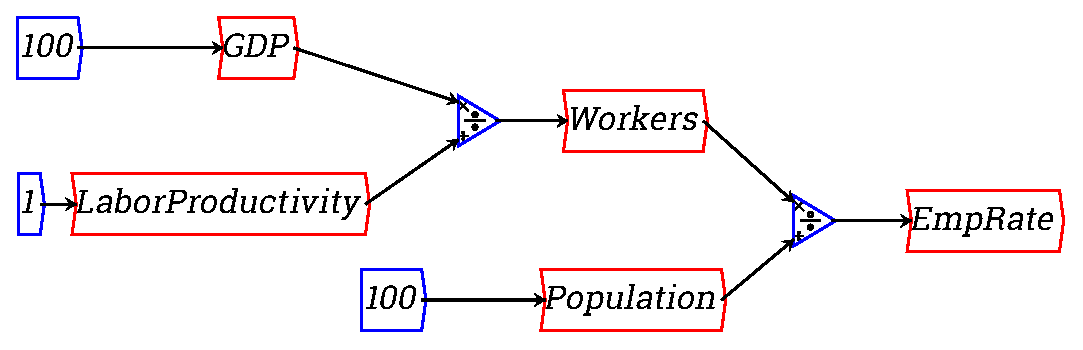
\includegraphics{images/NewItem1.eps}}
\end{center}

For a simple algebraic equation like this, modern computer algebra
programs like Mathcad are just as good as a block diagram programs like
Vissim or Minsky. But the visual metaphor excels when you want to describe a
complex causal chain.


These causal chains always involve a relationship between stocks and
flows. Economists normally model stocks and flows by adding an
increment to a stock. For example, the level of capital $K$ is defined as
a difference equation, where capital in year $t$ is shown as being 
capital in year $t-1$ plus the investment that took place that year:

\begin{displaymath}
K_t=K_{t-1}+I_{t-1}
\end{displaymath}

The problem with this approach is that in reality, capital is
accumulating on a daily, or even hourly, basis. It is better to model
stock as continuous quantities and for this reason, all stocks and
flows in Minsky are handled instead as integral equations. The amount
of capital at time $t$ is shown as the integral of net investment
between time 0 and today:

\begin{displaymath}
K(t)=\int_0^t I(s)ds
\end{displaymath}

However, rather than being shown as an equation, the relationship is shown as a diagram:

\begin{center}
\includegraphics{images/NewItem7.eps}
\end{center}

The advantages of the block diagram representation of dynamic equations
over a list of equations are:
\begin{itemize}
\item    They make the causal relationships in a complex model
  obvious. It takes a specialized mind to be able to see the causal
  relations in a large set of mathematical equations; the same
  equations laid out as diagrams can be read by anyone who can read
  a stock and flow diagram---and that's most of us;
\item The block diagram paradigm makes it possible to store components of
  a complex block diagram in a group. For example, the fuel delivery
  system in a car can be treated as one group, the engine as another,
  the exhaust as yet another. This reduces visual complexity and also
  makes it possible for different components of a complex model to be
  designed by different groups and then ``wired together'' at a later
  stage.
\end{itemize}

For example, here's a model of a 4 cylinder engine car---one of the
simple examples distributed with the program Vissim:

\begin{center}
\fwhtmladdimg{NewItem8.png}
\end{center}

Programs like Vissim and Simulink have been in existence for almost 2
decades, and they are now mature products that provide everything
their user-base of engineers want for modeling and analyzing complex
dynamic systems. \htmlref{So why has Minsky been
  developed?}{intro:experienced}

\section{Experienced in system dynamics?}
\label{intro:experienced}

As an experienced system dynamics user (or if you've just read \htmlref{``New to
system dynamics?''}{intro:new}), what you need to know is what Minsky
provides that other system dynamics programs don't. That boils down to
one feature: The Godley Table. It enables a dynamic model of
financial flows to be derived from a table that is very similar to the
accountant's double-entry bookkeeping table.


The dynamics in financial flows could be modeled using the block diagram
paradigm. But it would also be very, very easy to make a mistake
modeling financial flows in such a system, for one simple reason:
every financial flow needs to be entered at least twice in a
system---once as a source, and once as a sink.


For example, if you go shopping and buy a new computer with your
credit card, you increase your debt to a bank and simultaneously
increase the deposit account of the retailer from whom you buy the
computer. The two system states in this model---your credit card
(``BuyerCredit'') and the retailer's deposit account
(``SellerDeposit'')---therefore have to have the same entry (let's call
this ``Card'') made into them. Such a transaction would look
like this:


\begin{center}
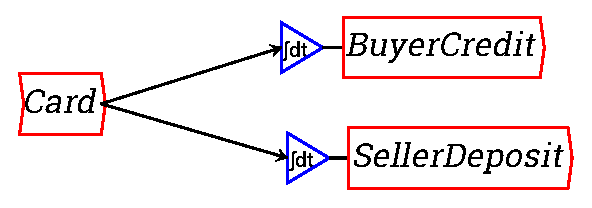
\includegraphics{images/NewItem11.eps}
\end{center}

That would work, but there's nothing in the program that warns you if
you make a mistake like, for example, wiring up the BuyerCredit entry,
but forgetting the SellerDeposit one:

\begin{center}
\includegraphics{images/NewItem12.eps}
\end{center}

Or, perhaps, wiring up both blocks, but giving one the wrong sign:

\begin{center}
\includegraphics{images/NewItem51.eps}
\end{center}

In a very complex model, you might make a mistake like one of the above, run the simulation and get nonsense results, and yet be unable to locate your mistake.


Minsky avoids this problem by using the paradigm that accountants
developed half a millennium ago to keep financial accounts accurately:
double-entry bookkeeping. Here is the same model in Minsky:

\begin{center}
\begin{tabular}{|c|cc|c|}
\hline
Flows $\downarrow$ / Stock Variables
$\rightarrow$&\multicolumn{1}{|c|}{$BuyerCredit$}&\multicolumn{1}{|c|}{$SellerDeposit$}&Row Sum\\\cline{2-3}&\multicolumn{1}{|c|}{asset}&\multicolumn{1}{|c|}{liability}&\\\hline
Initial Conditions&$0$&$0$&0\\
Buyer Accesses Credit&$Card$&$Card$&0\\
\hline
\end{tabular}
\end{center}

This is an inherently better way to generate a dynamic model of financial flows, for at least two reasons:
\begin{itemize}
\item All financial transactions are flows between entities. The
  tabular layout captures this in a very natural way: each row shows
  where a flow originates, and where it ends up
\item The program adopts the accounting practice of double-entry
  bookkeeping, in which entries on each row balance to zero according
  to the {\em accounting equation} (Assets=Liabilities+Equities). The source is
  shown as a positive value increasing the value of assets, the sink
  is a positive value increasing a corresponding liability. If you
  don't ensure that each flow starts somewhere and ends
  somewhere---say you make the same mistake as in the block diagram
  examples above, then the program will identify your mistake.
\end{itemize}

If you forget to enter the recipient in this transaction, then the Row
Sum identifies your mistake by showing that the row sums to ``Card''
rather than zero:

\begin{center}
\begin{tabular}{|c|cc|c|}
\hline
Flows $\downarrow$ / Stock Variables
$\rightarrow$&\multicolumn{1}{|c|}{$BuyerCredit$}&\multicolumn{1}{|c|}{$SellerDeposit$}&Row Sum\\\cline{2-3}&\multicolumn{1}{|c|}{asset}&\multicolumn{1}{|c|}{liability}&\\\hline
Initial Conditions&$0$&$0$&0\\
Buyer Accesses Credit&$Card$&&$Card$\\
\hline
\end{tabular}
\end{center}

And it also identifies if you give the wrong sign to one entry:

\begin{center}
\begin{tabular}{|c|cc|c|}
\hline
Flows $\downarrow$ / Stock Variables
$\rightarrow$&\multicolumn{1}{|c|}{$BuyerCredit$}&\multicolumn{1}{|c|}{$SellerDeposit$}&Row Sum\\\cline{2-3}&\multicolumn{1}{|c|}{asset}&\multicolumn{1}{|c|}{liability}&\\\hline
Initial Conditions&$0$&$0$&0\\
Buyer Accesses Credit&$Card$&$-Card$&$2Card$\\
\hline
\end{tabular}
\end{center}

Minsky thus adds an element to the system dynamics toolkit which is
fundamental for modeling the monetary flows that are an intrinsic
aspect of a market economy. Future releases will dramatically extend
this capability. 


\include{GettingStarted-Minsky}

\chapter{Minsky Tutorial}

\label{tutorial-Minsky}

\section{Basic System Dynamics model}

In 1965, Richard Goodwin, the great pioneer of complexity in economics,
presented the paper \htmladdnormallink{``A Growth Cycle''}{https://en.wikipedia.org/wiki/Goodwinmodel(economics)}
to the First World Congress of the Econometric Society in Rome. It
was later published in a book collection (Goodwin, Richard M. 1967.
"A Growth Cycle," in C. H. Feinstein, {\em Socialism, Capitalism
and Economic Growth}. Cambridge: Cambridge University Press, pp.
54--58.); to my knowledge it was never published in a journal.

Goodwin's model has been subjected to much critical literature about
implying stable cycles, not matching empirical data, etc., but Goodwin
himself emphasized that it was a ``starkly schematized and hence
quite unrealistic model of cycles in growth rates". He argued however
that it was a better foundation for a more realistic model than ``the
more usual treatment of growth theory or of cycle theory, separately
or in combination.''

Goodwin emphasized the similarity of this model to the Lokta-Volterra
model of interacting predator and prey, which can make it seem as
if it was derived by analogy to the biological model. But in fact
it can easily be derived from a highly simplified causal chain:
\begin{itemize}
\item The level of output ($Y$) determines the level of employment ($L$),
with $L=Y/a$ where $a$ is a measure of labor productivity; 
\item Given a population $N$, the employment rate $\lambda=L/N$ plays
a role in determining the \textbf{\em rate of change} of the wage
$w$: Goodwin used a linear approximation to a non-linear ``Phillips
Curve'':

%\fwhtmladdimg{NewItem55.png}

\begin{center}
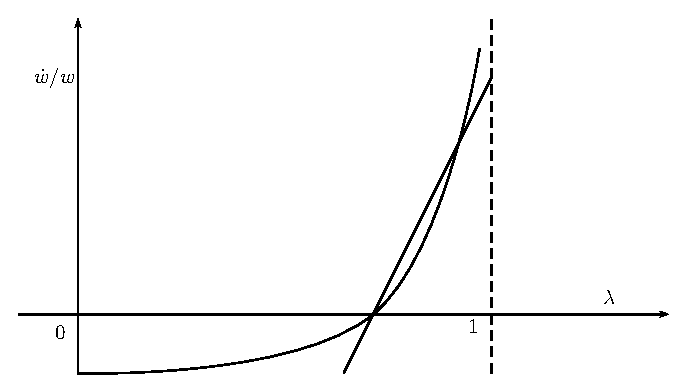
\includegraphics{images/PhillipsCurve} 
\par\end{center}

His linear approximation was:

\[
\frac{1}{w}\frac{d}{dt}w=-\gamma+\rho\cdot\lambda
\]

\item In a simple two-class model, profits $\Pi$ equals the level of output
$Y$ minus the wage bill: $\Pi=Y-wL$ 
\item For simplicity, Goodwin assumed that all profits were invested, so
that Investment equals profits: $I=\Pi$. 
\item Investment is the rate of change of the capital stock $K$; 
\item The level of output is, to a first approximation, determined by the
level of capital stock ($K$). A simple way of stating this is that
$Y$ is proportional to $K$: $Y=K/v$, where $v$ is a constant (Goodwin
notes that this relation ``could be softened but it would mean a
serious complicating of the structure of the model''); and finally 
\item Goodwin assumed that labor productivity grew at a constant rate $\alpha$,
while population grew at a constant rate $\beta$.

Goodwin published the model as a reduced form equation in the two
system states the employment rate ($\lambda$) and the workers' share
of output ($\omega$):

\begin{eqnarray*}
\frac{d}{dt}\lambda & = & \lambda\left(\frac{1-\omega}{v}-\alpha-\beta\right)\\
\frac{d}{dt}\omega & = & \omega\cdot\left(\rho\cdot\lambda-\gamma-\alpha\right)
\end{eqnarray*}

\end{itemize}
This form is useful for analytic reasons, but it obscures the causal
chain that actually lies behind the model. With modern system dynamic
software, this can be laid out explicitly, and we can also use much
more meaningful names. We'll start with defining output (which is
a variable). Click on \buttonIcon{var.eps} on the Icon Palette,
or click on the Operations menu and choose ``Variable''. This will
open up the ``Specify Variable Name'' window:
\begin{center}
\scalebox{0.5}{\htmladdimg{NewItem63.png}} 
\par\end{center}

Enter ``{\em\textbf{GDP}'' into the ``Name'' field, and leave
the other fields blank---since {\emGDP} is a variable and we're
defining a dynamic system, the value of {\emGDP} at any particular
point in time will depend on the other entities in the model. Now
Click OK (or press ``Enter''). The variable will now appear, attached
to the cursor. Move to a point near the top of the screen and click,
which will place the variable at that location.}

We are now going to write the first part of the model, that Labor
({\em\textbf{Labor}) equals output ({\emGDP}) divided by labor
productivity ({\emLabProd}). Just for the sake of illustration,
we'll make {\ema} a parameter, which is a named constant (this
can easily be modified later). For this we start by clicking on \buttonIcon{const.eps}
on the Palette, or by choosing Insert/variable from the menu. This
will pop-up the Edit Constant window:}
\begin{center}
\scalebox{0.5}{\htmladdimg{NewItem66.png}} 
\par\end{center}

There is actually no real difference between the ``Edit constant''
dialog and the ``Edit variable'' dialog. The window's title differs,
and the default value of Type is ``constant'' instead of ``flow''.
We're going to select ``parameter'', allowing one to give the parameter
a name.

Give the paramter the name ``{\em\textbf{LabProd}'' and the value
of 1 (i.e., one unit of output per worker). Click OK or press Enter
and the constant \buttonIcon{LabProd.eps} will now be attached to
the cursor. Place it below {\emGDP}:}
\begin{center}
\scalebox{0.5}{\htmladdimg{NewItem66.png}} 
\par\end{center}

Now we need to divide {\em\textbf{GDP} by {\emLabProd}. Click
on the \buttonIcon{divide.eps} symbol on the palette and the symbol
will be attached to the cursor. Drag it near the other two objects
and click. Your Canvas will now look something like this:}
\begin{center}
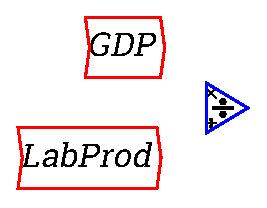
\includegraphics{images/NewItem70} 
\par\end{center}

Now to complete the equation, you have to attach {\em\textbf{GDP}
to the top of the divide block and LabProd to the bottom.}

Now move your cursor to the right hand side of \buttonIcon{GDP.eps}
and click, hold the mouse button down, and drag. An arrow will come
out from \buttonIcon{GDP.eps}. Drag this arrow to the top of the
divide block (where you'll see a tiny multiply sign) and release the
mouse. You should then see this:
\begin{center}
\includegraphics{images/NewItem74} 
\par\end{center}

When the mouse hovers over a block, you will then see little circles
that identify the input and output ports of the block:
\begin{center}
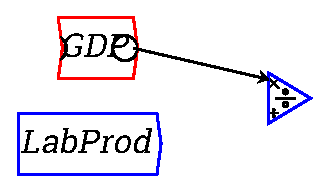
\includegraphics{images/NewItem75} 
\par\end{center}

Those are the connection points for wires, so start dragging from
one and release on the other. Now wire LabProd to the bottom of the
Divide block (where you'll see a miniature divide symbol (blown up
below):
\begin{center}
\includegraphics{images/NewItem76} 
\par\end{center}

Then click on \buttonIcon{var.eps} in the Design Icons to create
a new variable, call it Labor, place it the the right of the Divide
block, and wire the output port from the Divide block to the input
port for \textbf{\em Labor}:
\begin{center}
\includegraphics{images/NewItem79} 
\par\end{center}

To show the correspondence between the flowchart above and standard
modeling equations, click on the equations tab:

\begin{eqnarray*}
\mathrm{GDP} & =\\
\mathrm{Labor} & = & \frac{\mathrm{GDP}}{\mathrm{LabProd}}\\
\end{eqnarray*}

Now let's keep going with the model. With \textbf{\em Labor} defined,
the employment rate will be \textbf{\em Labor} divided by \textbf{\em
Population}. Define \textbf{\em Population} as a parameter (we'll
later change it to a variable), and give it a value of 110.
\begin{center}
\scalebox{0.5}{\htmladdimg{NewItem81.png}} 
\par\end{center}

Add it to the Canvas and you are now ready to define the employment
rate---another variable. Click on \buttonIcon{var.eps}, give it
the name ``$\backslash$lambda'' (be sure to include the backslash
symbol), put another Divide block on the canvas, choose Wire mode
and wire this next part of the model up. You should now have:
\begin{center}
\includegraphics{images/NewItem83} 
\par\end{center}

Now switch to the equations tab, and you will see

\begin{eqnarray*}
\mathrm{GDP} & =\\
\mathrm{Labor} & = & \frac{\mathrm{GDP}}{\mathrm{LabProd}}\\
\lambda & = & \frac{\mathrm{Labor}}{\mathrm{Population}}\\
\end{eqnarray*}

Notice that Minsky outputs a Greek $\lambda$ in the equation. You
can input such characters directly, if your keyboard supports them
as unicode characters, however you can also use a subset of the LaTeX
language to give your variables more mathematial names.

With the employment rate defined, we are now ready to define a ``Phillips
Curve'' relationship between the level of employment and the {\em\textbf{rate
of change} of wages. There was far more to Phillips than this (he
actually tried to introduce economists to system dynamics back in
the 1950s), and far more to his employment-wage change relation too,
and he insisted that the relationship was nonlinear (as in Goodwin's
figure above). But again for simplicity we'll define a linear relationship
between employment and the rate of change of wages.}

Here we need to manipulate the basic linear equation that Goodwin
used:

\[
\frac{1}{w}\frac{d}{dt}w=-\gamma+\rho\cdot\lambda
\]

Firstly multiply both sides by $w$:

\[
\frac{d}{dt}w=w\cdot(-\gamma+\rho\cdot\lambda)
\]

Then integrate both sides (because integration is a numerically much
more stable process than differentiation, all system dynamics programs
use integration rather than differentiation):

\[
w=w_{0}+\int w\cdot(-\gamma+\rho\cdot\lambda)
\]

In English, this says that the wage now is the initial wage plus the
integral of the wage multiplied by its rate of change function. That's
what we now need to add to the Canvas, and the first step is to spell
out the wage change function itself. Firstly, since we're using a
linear wage response function, the rate of employment has to be referenced
to a rate of employment at which the rate of changes is zero. I suggest
using Milton Friedman's concept of a ``Non-Accelerating-Inflation-Rate-of-Unemployment'',
or NAIRU. We need to define this constant, subtract it from 1, and
subtract the result from the actual employment rate $\lambda$. To
enter 1, click on \buttonIcon{const.eps}, define a constant and
give it a value of 1. Then define another variable NAIRU, and give
it a value of 0.05 (5\% unemployment). Select ``parameter'' as the
variable type. Subtract this from 1 and subtract the result from $\lambda$.
You should have the following:
\begin{center}
\includegraphics{images/NewItem108} 
\par\end{center}

Now we need to multiply this gap between the actual employment rate
and the ``NAIRE'' rate by a parameter that represents the response
of wages to this gap. Let's call this parameter \textbf{\em Emp\_\{Response\}}
(remember to include the underscore and the braces). Define the parameter,
give it a value of 10, and multiply ($\lambda$ minus NAIRE) by it:
\begin{center}
\resizebox{\textwidth}{!}{\includegraphics{images/NewItem109}} 
\par\end{center}

Now we are ready to add a crucial component of a dynamic model: the
integral block, which takes a flow as its input and has the integral
of that flow as the output. The wage rate \textbf{\em w} is such
a variable, and we define it by clicking on the \buttonIcon{int.eps}
symbol in the Icon Palette (or by choosing Operations/Integrate from
the {\em Insert} menu). This then attaches the following block
to the cursor:
\begin{center}
\includegraphics{images/NewItem39} 
\par\end{center}

Now we need to rename this from the default name of ``int1'' to
``{\em\textbf{w}'' for the wage rate. Either right click or double-click
on ``int1'' and this will bring up the edit window . Rename it to
``w'' and give it a value of 1:}
\begin{center}
\scalebox{0.5}{\htmladdimg{NewItem93.png}} 
\par\end{center}

To compete the integral equation, we need to multiply the linear employment
response function by the current wage before we integrate it (see
the last equation above). There are two ways to do this. First, place
a multiply block between the wage change function and the integral
block, wire the function up to one input on the multiply block, and
then either:
\begin{itemize}
\item wire the output of the \textbf{\em w} block back to the other input
on multiply block; or 
\item Right-click on \textbf{\em w}, choose ``Copy Var'', place that
copy before the multiply block, and wire it up. 
\end{itemize}
The first method gives you this initial result:
\begin{center}
\includegraphics{images/NewItem110} 
\par\end{center}

That looks messy, but notice the blue dot on the wire? Click and drag
on that and you will turn the straight line connector into a curve:
\begin{center}
\resizebox{\textwidth}{!}{\includegraphics{images/NewItem111}} 
\par\end{center}

The second approach, which I personally prefer (it's neater, and it
precisely emulates the integral equation), yields this result:
\begin{center}
\resizebox{\textwidth}{!}{\includegraphics{images/NewItem112}} 
\par\end{center}

From this point on the model develops easily---``like money for
old rope'', as one of my maths lecturers used to say. Firstly if
we multiply the wage rate \textbf{\em w} by \textbf{\em Labor} we
get the {\em\textbf{Wage Bill}. To do this, firstly create the
variable Wage Bill, and put it well below where $w$ currently is
on your diagram:}
\begin{center}
\resizebox{\textwidth}{!}{\includegraphics{images/NewItem113}} 
\par\end{center}

Now right-click on \textbf{\em WageBill} and choose ``Flip''. This
rotates the block through 180 degrees (any arbitrary rotation can
be applied from the variable definition window itself). Now right-click
on \textbf{\em Labor}, which you've already defined some time ago,
and choose ``Copy''. Place the copy of \textbf{\em Labor} to the
right of \textbf{\em WageBill}:
\begin{center}
\includegraphics{images/NewItem98} 
\par\end{center}

Now insert a multiply block before \textbf{\em WageBill}, and wire
\textbf{\em w} and \textbf{\em Labor} up to it. Curve the wire from
$w$ using the blue dots (you can do this multiple times to create
a very curved path: each time you create a curve, another 2 curve
points are added that you can also manipulate, as I have done below:
\begin{center}
\resizebox{\textwidth}{!}{\includegraphics{images/NewItem114}} 
\par\end{center}

The next step is to subtract the \textbf{\em WageBill} from \textbf{\em
GDP} to define \textbf{\em Profits}. Take a copy of \textbf{\em
GDP}, insert it above \textbf{\em WageBill}, insert a subtract block,
and wire it up to define the variable \textbf{\em Profits}:
\begin{center}
\includegraphics{images/NewItem100} 
\par\end{center}

In the simple Goodwin model, all Profits are invested, and investment
of course is the rate of change of the capital stock Capital. Create
a variable called Investment, wire this up to Profits, and then create
a new integral variable {\em Capital} using the \buttonIcon{int.eps}
icon. Right-click or double-click on it to rename {\em int2} to
{\em Capital}, and give it an initial value of 300:
\begin{center}
\scalebox{0.5}{\htmladdimg{NewItem102.png}} 
\par\end{center}

Wire this up to Investment:
\begin{center}
\includegraphics{images/NewItem104} 
\par\end{center}

Now there's only one step left to complete the model: define a parameter
CapOutputRatio and give it a value of 3:
\begin{center}
\scalebox{0.5}{\htmladdimg{NewItem103.png}} 
\par\end{center}

Divide Capital by this, and wire the result up to the input on GDP.
You have now built your first dynamic model in Minsky:

Before you attempt to run it, do two things. Firstly from the {\em
Runge Kutta} menu item, change the Max Step Size to 0.01---to get
a smoother simulation.
\begin{center}
\scalebox{0.5}{\htmladdimg{NewItem107.png}} 
\par\end{center}

Secondly, add some graphs by clicking on the \smhtmladdimg{plot.png}
icon, placing the graph in the middle of the flowchart, and wiring
up $\lambda$ and $w$ to two of the four inputs on the left hand
side. You will now see that, rather than reaching equilibrium, the
model cycles constantly:
\begin{center}
\resizebox{\textwidth}{!}{\includegraphics{images/NewItem116}} 
\par\end{center}

If you click on the equations tab, you will see that you have defined
the following system of equations:

\begin{eqnarray*}
\mathrm{GDP} & = & \frac{\mathrm{Capital}}{\mathrm{CapOutRatio}}\\
\mathrm{Investment} & = & \mathrm{Profits}\\
\mathrm{Labor} & = & \frac{\mathrm{GDP}}{\mathrm{LabProd}}\\
\mathrm{Profits} & = & \mathrm{GDP}-\mathrm{WageBill}\\
\mathrm{WageBill} & = & w\times\mathrm{Labor}\\
\lambda & = & \frac{\mathrm{Labor}}{\mathrm{Population}}\\
\omega & = & \frac{\mathrm{WageBill}}{\mathrm{GDP}}\\
\frac{dw}{dt} & = & \mathrm{Emp}_{\mathrm{Response}}\times(\lambda-(1-\mathrm{NAIRU})\times w\\
\frac{d\mathrm{Capital}}{dt} & = & \mathrm{Investment}\\
\end{eqnarray*}

At this level of complexity, the equation form---if you're accustomed
to working in equations---is as accessible as the block diagram model
from which it was generated. But at much higher levels of complexity,
the block diagram is far easier to understand since it displays the
causal links in the model clearly, and can be structured in sub-groups
that focus on particular parts of the system.

\section{Basic Banking model}

\label{tut:basicBankModel}

If you haven't yet read the section on \htmlref{Creating a Banking
Model}{creatingBankingModel}, do so now. This tutorial starts from
the skeleton of the ``Loanable Funds'' model built in that section,
and using \htmlref{time constants}{time-constants} to specify
how quickly lending occurs.

\subsection{Loanable Funds}

Our model begins with the single operation of Patient lending to Impatient
at a rate that, if kept constant at its initial level of of \$10 per
annum, would empty the Patient account in 10 years. Because the rate
of outflow declines as the Patient account declines, the money in
the account decays towards zero but never quite reaches it.

%\begin{center}
%\begin{tabular}{|c|cccc|}
%\hline
%Flows $\downarrow$ / Stock Variables $\rightarrow$&\multicolumn{1}{|c|}{$Reserves$}&\multicolumn{1}{|c|}{$Patient$}&\multicolumn{1}{|c|}{$Impatient$}&\multicolumn{1}{|c|}{$Safe$}\\\cline{2-5}&\multicolumn{1}{|c|}{asset}&\multicolumn{2}{|c|}{liability}&\multicolumn{1}{|c|}{equity}\\\hline
%Initial Conditions&$120$&$100$&$0$&$20$\\
%Patient lends to Impatient&&$-Lend$&$Lend$&\\
%\hline
%\end{tabular}
%\resizebox{\textwidth}{!}{\includegraphics{images/NewItem169.eps}}
%\end{center}

\begin{center}
\scalebox{.5}{\includegraphics{images/godleyTableWithAccounts5}} 
\par\end{center}

Many more actions need to be added to this model to complete it. For
a start, Impatient should be paying interest to Patient on the amount
lent. Add an additional row to the Godley Table by clicking on the
`+' key next to ``Patient lends to Impatient'' to create a blank
row:

%\begin{center}
%\begin{tabular}{|c|cccc|}
%\hline
%Flows $\downarrow$ / Stock Variables $\rightarrow$&\multicolumn{1}{|c|}{$Reserves$}&\multicolumn{1}{|c|}{$Patient$}&\multicolumn{1}{|c|}{$Impatient$}&\multicolumn{1}{|c|}{$Safe$}\\\cline{2-5}&\multicolumn{1}{|c|}{asset}&\multicolumn{2}{|c|}{liability}&\multicolumn{1}{|c|}{equity}\\\hline
%Initial Conditions&$120$&$100$&$0$&$20$\\
%Patient lends to Impatient&&$-Lend$&$Lend$&\\
%&&&&\\
%\hline
%\end{tabular}
%\end{center}

\begin{center}
\scalebox{.5}{\includegraphics{images/godleyTableWithAccounts6}} 
\par\end{center}

Then label this flow ``Impatient pays interest'' and make the entry
``Interest'' into the cell for Patient on that row. Make the matching
entry ``-Interest'' in the cell for Impatient. The flow ``Interest''
now appears on the input side of the Godley Table on the Canvas:

%\begin{center}
%\begin{tabular}{|c|cccc|}
%\hline
%Flows $\downarrow$ / Stock Variables $\rightarrow$&\multicolumn{1}{|c|}{$Reserves$}&\multicolumn{1}{|c|}{$Patient$}&\multicolumn{1}{|c|}{$Impatient$}&\multicolumn{1}{|c|}{$Safe$}\\\cline{2-5}&\multicolumn{1}{|c|}{asset}&\multicolumn{2}{|c|}{liability}&\multicolumn{1}{|c|}{equity}\\\hline
%Initial Conditions&$120$&$100$&$0$&$20$\\
%Patient lends to Impatient&&$-Lend$&$Lend$&\\
%Impatient pays interest&&$Interest$&$-Interest$&\\
%\hline
%\end{tabular}
%\end{center}

\begin{center}
\scalebox{.5}{\includegraphics{images/godleyTableWithAccounts7}} 
\par\end{center}

Interest now has to be defined. It will be the amount in Impatient's
account (since this began at zero) multiplied by the rate of interest
charged by Patient:
\begin{center}
\includegraphics{images/NewItem173} 
\par\end{center}

With that definition, the dynamics of the model change: rather than
the Patient account falling to zero and Impatient rising to 100, the
two accounts stabilize once the outflow of new loans by Patient equals
the inflow of interest payments by Impatient:
\begin{center}
\resizebox{\textwidth}{!}{\includegraphics{images/NewItem174}} 
\par\end{center}

Though it stabilizes, this is is still a very incomplete model: neither
Patient nor Impatient are doing anything with the money apart from
lending it and paying interest. I am now going to assume that Impatient
is borrowing the money in order to hire workers to work at a factory
and produce output for sale. So we now need another account called
Workers, and a payment from Impatient to Workers called Wage:

%{
%  \noindent
%\small
%\begin{tabular}{|c|ccccc|}
%\hline
%Flows $\downarrow$ / Stock Variables $\rightarrow$&\multicolumn{1}{|c|}{$Reserves$}&\multicolumn{1}{|c|}{$Patient$}&\multicolumn{1}{|c|}{$Impatient$}&\multicolumn{1}{|c|}{$Workers$}&\multicolumn{1}{|c|}{$Safe$}\\\cline{2-6}&\multicolumn{1}{|c|}{asset}&\multicolumn{3}{|c|}{liability}&\multicolumn{1}{|c|}{equity}\\\hline
%Initial Conditions&$120$&$100$&$0$&$0$&$20$\\
%Patient lends to Impatient&&$-Lend$&$Lend$&&\\
%Impatient pays interest&&$Interest$&$-Interest$&&\\
%Impatient pays Workers&&&$-Wage$&$Wage$&\\
%\hline
%\end{tabular}
%}

\begin{center}
\scalebox{.5}{\includegraphics{images/godleyTableWithAccounts8}} 
\par\end{center}

In a more complex model, the Wage bill could be related to the current
rate times the number of workers in employment. In this simple model
I will regard the wage as a function of the amount of money in Impatient's
account turning over several times a year in the payment of wages.
Using a time constant, I will assume that the amount in Impatient's
account turns over 3 times a year paying wages, so that the time constant
$\tau_{T}$ is 1/3rd of a year:
\begin{center}
\includegraphics{images/NewItem176} 
\par\end{center}

The dynamics of this incomplete model are very different again: very
little money turns up in the Impatient account, and all of the money
ends up in the Workers account. However economic activity also ceases
as both lending and the flow of wages falls towards zero:
\begin{center}
\resizebox{\textwidth}{!}{\includegraphics{images/NewItem177}} 
\par\end{center}

This is because wages are being paid to workers, but they are doing
nothing with it. So we need to include consumption by workers--and
by Patient as well. Here the reason time constants are useful may
be more obvious. The time constant for consumption by Workers is given
the very low value of 0.05---or 1/20th of a year---which indicates
that if their initial rate of consumption was maintained without any
wage income, they would reduce their bank balances to zero in 1/20th
of a year or about 2.5 weeks. 


% no FAQs have been answered yet :)
%\chapter{FAQs}

\section{Why no difference equations?}
\label{faq:no-difference}

\end{document}
